\documentclass[12pt,twoside]{mitthesis}
\usepackage{url}
\usepackage{epsfig}
\usepackage{reader}
\usepackage{times}
\usepackage{amsthm}
\usepackage{amsmath}
\usepackage{amssymb}
\usepackage{subfigure}
\usepackage{algorithm}
\usepackage{algpseudocode}
\usepackage{appendix}
\usepackage{color}
\usepackage[nolineno]{lgrind}
\usepackage[colorlinks=true,pdfstartview=FitV,
            linkcolor=linkcolor,citecolor=linkcolor,urlcolor=linkcolor]{hyperref}
\usepackage[all]{hypcap}
% replace courier with beramono, a fixed-width font that is more condensed
% see more fonts here:  http://www.tug.dk/FontCatalogue/
\usepackage[T1]{fontenc}
%\renewcommand*\ttdefault{lcmtt}    % Computer Modern Teletype L
%\renewcommand*\ttdefault{cmvtt}    % Computer Modern Teletype Proportional
\usepackage[scaled=0.88]{beramono}

% bold italic font
\newfont{\boldit}{cmbxti11}
\newfont{\boldslant}{cmbxsl11}

% the color of all my links
\definecolor{linkcolor}{rgb}{0,0,0}  % FOR PRINTING
%\definecolor{linkcolor}{rgb}{0,0,1}  % FOR WEB

% figure spacing...
% space between floats
\setlength{\floatsep}{36pt}
% space between last top float or first bottom float and the text
\setlength{\textfloatsep}{24pt}
% space above caption
%\setlength{\abovecaptionskip}{}
% space below caption
%\setlength{\belowcaptionskip}{}

% some handy font sizes
\newcommand{\sevenpoint}{\fontsize{7pt}{9pt}\selectfont}
\newcommand{\eightpoint}{\fontsize{8pt}{10pt}\selectfont}
\newcommand{\ninepoint}{\fontsize{9pt}{11pt}\selectfont}
\newcommand{\tenpoint}{\fontsize{10pt}{12pt}\selectfont}
\newcommand{\elevenpoint}{\fontsize{11pt}{13pt}\selectfont}
\newcommand{\twelvepoint}{\fontsize{12pt}{14pt}\selectfont}
\newcommand{\thirteenpoint}{\fontsize{13pt}{15pt}\selectfont}
\newcommand{\fourteenpoint}{\fontsize{14pt}{16pt}\selectfont}
\newcommand{\fifteenpoint}{\fontsize{15pt}{17pt}\selectfont}

% do not indent paragraphs of enumerated lists (my lists go on for pages...)
% numbers flush left to paragraph text: \leftmargin=17pt
\newcommand{\mybegin}{\begin{list}{\labelenumi}{\leftmargin=\parindent}\usecounter{enumi}}
\newcommand{\myitem}[1]{\item {\boldslant #1}}
\newcommand{\myend}{\end{list}}

% shrink section titles
\makeatletter
\def\section{\@startsection {section}{1}{\z@}%
  {-3.5ex \@plus -1ex \@minus -.2ex}%
  {2.3ex \@plus.2ex}%
  {\normalfont\fifteenpoint\bfseries}}
\makeatother

% shrink sub-section titles
\makeatletter
\def\subsection{\@startsection{subsection}{2}{\z@}%
  {-3.25ex\@plus -1ex \@minus -.2ex}%
  {1.5ex \@plus .2ex}%
  {\normalfont\thirteenpoint\bfseries}}
\makeatother

% use same counter for figures and tables
\makeatletter
\let\c@figure\c@table % or vice-versa
\let\c@lof\c@lot % or vice-versa
\def\ftype@table{1}%
\makeatother

% do not list sub-sub sections in table of contents
\setcounter{tocdepth}{1}

% use this instead of \chapter to add chapter titles to list of figures
\newcommand{\startchapter}[1]{\chapter{#1}\addcontentsline{lof}{figure}{\hspace{-18pt}{\bf \thechapter \hspace{9.5pt} #1}}}

% fix marginpar so text stays on the page
\setlength{\marginparwidth}{0.8in}
\let\oldmarginpar\marginpar
\renewcommand\marginpar[1]{\-\oldmarginpar[\raggedleft\footnotesize #1]%
{\raggedright\footnotesize #1}}

% used to write notes to advisor.  convert to blank command for final copy.
%\newcommand{\note}[1]{\marginpar{\color{red} #1}}
\newcommand{\note}[1]{}

\pagestyle{plain}

% ----------------------------------------------------------------------

% date I'm handing in
\newcommand{\mydate}[0]{January 30, 2009}

% for my thesis only:  need sdep as early as intro an dtable of contents
\newcommand{\sdep}[0]{\textsc{sdep}}
\newcommand{\sdepf}[2]{\sdep_{#1 \small{\leftarrow} #2}}
\newcommand{\mt}[1]{\mbox{\it #1}}
\newcommand{\figsdep}[0]{\mt{SDEP}}
\newcommand{\figsdepf}[2]{\mt{SDEP}_{#1 \small{\leftarrow} #2}}

\begin{document}

% -*-latex-*-
% $Log: not supported by cvs2svn $
% Revision 1.7  2001/02/08 18:53:16  boojum
% changed some \newpages to \cleardoublepages
%
% Revision 1.6  1999/10/21 14:49:31  boojum
% changed comment referring to documentstyle
%
% Revision 1.5  1999/10/21 14:39:04  boojum
% *** empty log message ***
%
% Revision 1.4  1997/04/18  17:54:10  othomas
% added page numbers on abstract and cover, and made 1 abstract
% page the default rather than 2.  (anne hunter tells me this
% is the new institute standard.)
%
% Revision 1.4  1997/04/18  17:54:10  othomas
% added page numbers on abstract and cover, and made 1 abstract
% page the default rather than 2.  (anne hunter tells me this
% is the new institute standard.)
%
% Revision 1.3  93/05/17  17:06:29  starflt
% Added acknowledgements section (suggested by tompalka)
%
% Revision 1.2  92/04/22  13:13:13  epeisach
% Fixes for 1991 course 6 requirements
% Phrase "and to grant others the right to do so" has been added to
% permission clause
% Second copy of abstract is not counted as separate pages so numbering works
% out
%
% Revision 1.1  92/04/22  13:08:20  epeisach
\title{Language and Compiler Support for Stream Programs}

\author{William Thies}
\department{Department of Electrical Engineering and Computer Science}
% If the thesis is for two degrees simultaneously, list them both
% separated by \and like this:
% \degree{Doctor of Philosophy \and Master of Science}
%\degree{Doctor of Philosophy of Science in Computer Science and Engineering}
\degree{Doctor of Philosophy}
\degreemonth{September} \degreeyear{2008} \thesisdate{\today}

\prevdegrees{~ \\ 
Bachelor of Science, Computer Science and Engineering\\
Massachusetts Institute of Technology, 2001 \\
~ \\
Bachelor of Science, Mathematics\\
Massachusetts Institute of Technology, 2002 \\
~ \\
Master of Engineering, Computer Science and Engineering \\
Massachusetts Institute of Technology, 2002 \\
~ \\
}

%% By default, the thesis will be copyrighted to MIT.  If you need to copyright
%% the thesis to yourself, just specify the `vi' documentclass option.  If for
%% some reason you want to exactly specify the copyright notice text, you can
%% use the \copyrightnoticetext command.
%\copyrightnoticetext{\copyright IBM, 1990.  Do not open till Xmas.}

% If there is more than one supervisor, use the \supervisor command
% once for each.
\supervisor{Saman Amarasinghe}{Associate Professor}

% These are optional, and enabled with reader.sty
%\reader{Arvind}{Professor}
%\reader{Srini Devadas}{Professor}

% This is the department committee chairman, not the thesis committee
% chairman.  You should replace this with your Department's Committee
% Chairman.
\chairman{Terry P. Orlando}{Chair, Department Committee on Graduate Students}

% Make the titlepage based on the above information.  If you need
% something special and can't use the standard form, you can specify
% the exact text of the titlepage yourself.  Put it in a titlepage
% environment and leave blank lines where you want vertical space.
% The spaces will be adjusted to fill the entire page.  The dotted
% lines for the signatures are made with the \signature command.
\maketitle

% The abstractpage environment sets up everything on the page except
% the text itself.  The title and other header material are put at the
% top of the page, and the supervisors are listed at the bottom.  A
% new page is begun both before and after.  Of course, an abstract may
% be more than one page itself.  If you need more control over the
% format of the page, you can use the abstract environment, which puts
% the word "Abstract" at the beginning and single spaces its text.

%% You can either \input (*not* \include) your abstract file, or you can put
%% the text of the abstract directly between the \begin{abstractpage} and
%% \end{abstractpage} commands.

% First copy: start a new page, and save the page number.
\cleardoublepage
% Uncomment the next line if you do NOT want a page number on your
% abstract and acknowledgments pages.
% \pagestyle{empty}
\setcounter{savepage}{\thepage}
\begin{abstractpage}
As DSP programming is becoming more complex, there is an increasing
need for high-level abstractions that can be efficiently compiled.
Toward this end, we present a set of aggressive optimizations that
target linear sections of a stream program.  Our input language is
StreamIt, which represents programs as a hierarchical graph of
autonomous filters.  A filter is linear if each of its outputs can be
represented as an affine combination of its inputs.  Linear filters
are common in DSP applications; examples include FIR filters,
expanders, compressors, FFTs and DCTs.

We present a linear extraction analysis that automatically detects
linear filters based on the C-like code in their {\tt work} function.
Once linear filters are identified, we show how neighboring nodes can
be collapsed into a single linear representation, thereby eliminating
many redundant computations.  Also, we describe a method for
automatically translating linear nodes into the frequency domain,
thereby yielding algorithmic savings for convolutional filters.

We have completed a fully-automatic implementation of the above
techniques as part of the StreamIt compiler, and we demonstrate
performance improvements that average 400\% over our benchmark
applications.




\end{abstractpage}

% Additional copy: start a new page, and reset the page number.  This way,
% the second copy of the abstract is not counted as separate pages.
% Uncomment the next 6 lines if you need two copies of the abstract
% page.
% \setcounter{page}{\thesavepage}
% \begin{abstractpage}
% As DSP programming is becoming more complex, there is an increasing
need for high-level abstractions that can be efficiently compiled.
Toward this end, we present a set of aggressive optimizations that
target linear sections of a stream program.  Our input language is
StreamIt, which represents programs as a hierarchical graph of
autonomous filters.  A filter is linear if each of its outputs can be
represented as an affine combination of its inputs.  Linear filters
are common in DSP applications; examples include FIR filters,
expanders, compressors, FFTs and DCTs.

We present a linear extraction analysis that automatically detects
linear filters based on the C-like code in their {\tt work} function.
Once linear filters are identified, we show how neighboring nodes can
be collapsed into a single linear representation, thereby eliminating
many redundant computations.  Also, we describe a method for
automatically translating linear nodes into the frequency domain,
thereby yielding algorithmic savings for convolutional filters.

We have completed a fully-automatic implementation of the above
techniques as part of the StreamIt compiler, and we demonstrate
performance improvements that average 400\% over our benchmark
applications.




% \end{abstractpage}

\cleardoublepage

\newpage
~ \vspace{-3.7\baselineskip}\\
\enlargethispage{0.3\baselineskip}
\section*{Acknowledgments}

I would like to start by expressing my deepest gratitude to my
advisor, colleague and friend, Saman Amarasinghe.
%Saman's committment to me has been downright scary.
%Simply put, Saman has changed my life.
%Simply put, Saman has been the mentor of a lifetime.
From 4am phone calls in Boston to weeks of one-on-one time in Sri
Lanka and India, Saman invested {\it unfathomable} time and energy
into my development as a researcher and as a person.  His extreme
creativity, energy, and optimism (not to mention mad PowerPoint
skills!) have been a constant source of inspiration, and whenever I am
at my best, it is usually because I am asking myself: {\it What would
Saman do}?  Saman offered unprecedented freedom for me to pursue
diverse interests in graduate school -- including weeks at a time
working with other groups -- and served as a fierce champion on my
behalf in every possible way.  I will forever treasure our deep sense
of shared purpose and can only aspire to impact others as much as he
has impacted me.

%Like a Papa Bear, any arguments between the two of us would be 
%completely dwarfed by the fierce battles he would wage on my behalf.

\vspace{-8pt}\paragraph*{Contributors to this dissertation} Many
people made direct contributions to the content of this dissertation.
The StreamIt project was a fundamentally collaborative undertaking,
involving the extended efforts of over 27 people.  I feel very lucky
to have been part of such an insightful, dedicated, and fun team.
Section~\ref{sec:streamit-project} provides a technical overview of
the entire project, including the division of labor.  In what follows
I am listing only a subset of each person's actual contributions.
Michael Gordon, my kindred Ph.D. student throughout the entire
StreamIt project, led the development of the parallelization
algorithms (summarized in Chapter~4), the Raw backend and countless
other aspects of the compiler.  Rodric Rabbah championed the project
in many capacities, including contributions to cache optimizations
(summarized in Chapter~4), teleport messaging (Chapter~3), the MPEG2
benchmarks, an Eclipse interface, and the Cell backend.  Michal
Karczmarek was instrumental in the original language design (Chapter
2) and teleport messaging, and also implemented the StreamIt scheduler
and runtime library.  David Maze, Jasper Lin, and Allyn Dimock made
sweeping contributions to the compiler infrastructure; I will forever
admire their skills and tenacity in making everything work.

Central to the StreamIt project is an exceptional array of
M.Eng. students, who I feel very privileged to have interacted with
over the years.  Andrew Lamb, Sitij Agrawal, and Janis Sermulins led
the respective development of linear optimizations, linear statespace
optimizations, and cache optimizations (all summarized in Chapter~4).
Janis also implemented the cluster backend, with support for teleport
messaging (providing results for Chapter~3).  Matthew Drake
implemented the MPEG2 codec in StreamIt, while Jiawen Chen implemented
a flexible graphics pipeline and Basier Aziz implemented mosaic
imaging.  Daviz Zhang developed a lightweight streaming layer for the
Cell processor; Kimberly Kuo developed an Eclipse user interface for
StreamIt; Juan Reyes developed a graphical editor for stream graphs;
and Jeremy Wong modeled the scalability of stream programs.  Kunal
Agrawal investigated bit-level optimizations in StreamIt.  Ceryen Tan
is improving StreamIt's multicore backend.

The StreamIt project also benefited from an outstanding set of
undergraduate researchers, who taught me many things.  Ali Meli, Chris
Leger, Satish Ramaswamy, Matt Brown, and Shirley Fung made important
contributions to the StreamIt benchmark suite (detailed in Chapter~2).
Steve Hall integrated compressed-domain transformations into the
StreamIt compiler (providing results for Chapter~5).  Qiuyuan Li
worked on a StreamIt backends for Cell, while Phil Sung targeted a
GPU.

%Qiuyuan Li worked on a StreamIt backend for the Cell processor, while
%Phil Sung worked on a backend for graphics processors.

Individuals from other research groups also impacted the StreamIt
project.  Members of the Raw group offered incredible support for our
experiments, including Anant Agarwal, Michael Taylor, Walter Lee,
Jason Miller, Ian Bratt, Jonathan Eastep, David Wentzlaff, Ben
Greenwald, Hank Hoffmann, Paul Johnson, Jason Kim, Jim Psota, Nathan
Schnidman, and Matthew Frank.
%
\newpage
\enlargethispage{0.3\baselineskip}
%
~ \vspace{-1.3\baselineskip}\\
\noindent Hank Hoffmann, Nathan Schnidman, and Stephanie Seneff also
provided valuable expertise on designing and parallelizing signal
processing applications.  External contributors to the StreamIt
benchmark suite include Ola Johnsson, Mani Narayanan, Magnus
Stenemo, Jinwoo Suh, Zain ul-Abdin, and Amy Williams.  Fabrice
Rastello offered key insights for improving our cache optimizations.
Weng-Fai Wong offered guidance on several projects during his visit
to the group.  StreamIt also benefited immensely from regular and
insightful conversations with stakeholders from industry, including
Peter Mattson, Richard Lethin, John Chapin, Vanu Bose, and Andy Ong.

Outside of the StreamIt project, additional individuals made direct
contributions to this dissertation.  In developing our tool for
extracting stream parallelism (Chapter~6), I am indebted to Vikram
Chandrasekhar for months of tenacious hacking and to Stephen McCamant
for help with Valgrind.  I thank Jason Ansel, Chen Ding, Ronny
Krashinsky, Viktor Kuncak, and Alex Salcianu, who provided valuable
feedback on manuscripts that were incorporated into this dissertation.
I am also grateful to Arvind and Srini Devadas for serving on my
committee on very short notice, and to Marek Olszewski for serving as
my remote agent of thesis submission!

\vspace{-8pt}\paragraph*{The rest of the story} Throughout my life,
I have been extremely fortunate to have had an amazing set of
mentors who invested a lot of themselves in my personal growth.  I
thank Thomas ``Doc'' Arnold for taking an interest in a nerdy high
school kid, and for setting him loose with chemistry equipment in a
Norwegian glacier valley -- a tactic which cemented my interest in
science, especially the kind you can do while remaining dry.
%a tactic which ignited not only my interest in science, but also in
%girls.
I thank Scott Camazine for taking a chance on a high school programmer
in my first taste of academic research, an enriching experience which
%was not only enriching and fun, but also 
opened up many doors for me in the future.  I thank Vanessa Colella
and Mitchel Resnick for making my first UROP experience a very
special one, as evidenced by my subsequent addiction to the UROP
program.  I thank Andrew Begel for teaching me many things, not
least of which is by demonstration of his staggering commitment,
capacity, and all-around coolness in mentoring undergraduates.  I'm
especially grateful to Brian Silverman, a mentor and valued friend
whose unique perspectives on everything from Life in StarLogo to
life on Mars have impacted me more than he might know.  I thank
Markus Zahn for excellent advice and guidance, both as my
undergraduate advisor and UROP supervisor.  Finally, I'm very
grateful to Kath Knobe, who provided unparalleled mentorship during
my summers at Compaq and stimulated my first interest in compilers
research.

Graduate school brought a new set of mentors.  I learned a great
deal from authoring papers or proposals with Anant Agarwal, Srini
Devadas, Fredo Durand, Michael Ernst, Todd Thorsen, and
Fr\'{e}d\'{e}ric Vivien, each of whom exemplifies the role of a
faculty member in nurturing student talent.  I am also very grateful
to Srini Devadas, Martin Rinard, Michael Ernst, and Arvind for being
especially accessible as counselors, showing interest in my work and
well-being even in spite of very busy schedules.  I could not have
imagined a more supportive environment for graduate study.

I thank Charles Leiserson and Piotr Indyk for teaching me about
teaching itself.  I will always remember riding the T with Charles
when a car full of Red Sox fans asked him what he does for a living.
Imagining the impressive spectrum of possible replies, I should not
have been surprised when Charles said simply, ``I teach''.  Nothing
could be more true, and I feel very privileged to have been a TA in
his class.

I'd like to thank my collaborators on projects other than StreamIt,
for enabling fulfilling and fun pursuits outside 
% the work described in 
of this dissertation.  In the microfluidics lab, I thank
J.P. Urbanski for many late nights ``chilling at the lab'', his
euphemism for a recurring process whereby he manufactures chips and
I destroy them.  His knowledge, determination, and overall good
nature are truly inspiring.  I also learned a great deal from David
Craig, Mats Cooper, Todd Thorsen, and Jeremy Gunawardena, 
%
\newpage
\enlargethispage{0.5\baselineskip}
%
~ \vspace{-1.5\baselineskip}\\
\noindent who were extremely supportive of our foray into
microfluidics.  I thank Nada Amin for her insights, skills, and
drive in developing our CAD tool, and for being an absolute pleasure
to work with.

%In the microfluidics lab, I learned an immense amount from
%J.P. Urbanski, microfluidic wizard extraordinaire whose work ethic
%is as intense as it is understated -- never again will I think
%lightly of a late night ``chilling at the lab''.

I'm very thankful to my collaborators in applying technology towards
problems in socio-economic development, from whom I've drawn much
support.  First and foremost is Manish Bhardwaj, whose rare
combination of brilliance, determination, and selflessness has been
a deep inspiration to me.  I also thank Emma Brunskill, who has been
a tremendous collaborator on many fronts, as well as
%whose independence and resourcefulness are always humbling.  
%I'm very grateful to Emma Brunskill, Somani Patnaik, 
Sara Cinnamon, Goutam Reddy, Somani Patnaik and Pallavi Kaushik for
being incredibly talented, dedicated, and fun teammates.
%I thank the Venerable Tenzin Priyadarshi and Scott Kennedy for
%valuable support and guidance.
%
%Further in the past, 
I am very grateful to Libby Levison for involving me in my first
project at the intersection of technology and development, without
which I might have gone down a very different path.  I also thank
Samidh Chakrabarti for being a great officemate and friend, and my
first peer with whom I could investigate this space together.

I am indebted to the many students and staff who worked with me on
the TEK project, including Marjorie Cheng, Tazeen Mahtab, Genevieve
Cuevas, Damon Berry, Saad Shakhshir, Janelle Prevost, Hongfei Tian,
Mark Halsey, and Libby Levison.  I also thank Pratik Kotkar,
Jonathan Birnbaum, and Matt Aasted for their work on the Audio Wiki.
I would not have been able to accomplish nearly as much without the
%continuous 
insights, dedication, and hard work of all these individuals.

% leaving out sri lanka guys, since it's not released:
% - Thayaparan Kailainathan
% - Mahendrakumar Senthivel
% - Thayarupan Rajendram
%
% leaving out some TEK authors who I don't even know:
% - Alexandro Artola
% - Binh D. Vo
% - Yuliya Litvak
% - Sheldon Chan
% - Sid Henderson

Graduate school would be nothing if not for paper deadlines, and I
feel very lucky to have been down in the trenches with such bright,
dependable, and entertaining co-authors.  Of people not already cited
as such, I thank Marten van Dijk, Blaise Gassend, Andrew Lee, Charles
W. O'Donnell, Kari Pulli, Christopher Rhodes, Jeffrey Sheldon, David
Wentzlaff, Amy Williams, and Matthias Zwicker for some of the best
end-to-end research experiences I could imagine.

Many people made the office a very special place to be.  Mary McDavitt
is an amazing force for good, serving as my rock and foundation
throughout many administrative hurricanes; I can't thank her enough
for all of her help, advice, and good cheer over the years.  I'm also
very grateful to Shireen Yadollahpour, Cornelia Colyer, and Jennifer
Tucker, whose helpfulness I will never forget.  Special thanks to
Michael Vezza, system administrator extraordinaire, for his extreme
patience and helpfulness in tending to my every question, and fixing
everything that I broke.

I thank all the talented members of the Commit group, and especially
the Ph.D. students and staff -- Jason Ansel, Derek Bruening, Vikram
Chandrasekhar, Gleb Chuvpilo, Allyn Dimock, Michael Gordon, David
Maze, Michal Karczmarek, Sam Larsen, Marek Olszewski, Diego Puppin,
Rodric Rabbah, Mark Stephenson, Jean Yang, and Qin Zhao.  On top of
tolerating {\it way} more than their fair share of StreamIt talks,
they offered the best meeting, eating, and traveling company ever.  I
especially thank Michael Gordon, my officemate and trusted friend, for
making 32-G890 one of my favorite places -- I'm really going to miss
our conversations (and productive silences!)

I'd like to extend special thanks to those who supported me in my job
search last spring.  I feel very grateful for the thoughtful counsel
of dozens of people on the interview trail, and especially to a few
individuals (you know who you are) who spent many hours talking to me
and advocating on my behalf.  This meant a great deal to me.  I also
thank Kentaro Toyama and others at MSR India for being very flexible
with my start date, as the submission of this thesis was gradually
postponed!

I am extremely fortunate to have had a wonderful support network to
sustain me throughout graduate school.  To the handful of close
friends who joined me for food, walks around town, or kept in touch
from a distance: thank you for seeing me through the thick and thin.
I'd like to especially call out to David Wentzlaff, Kunal Agrawal,
Michael Gordon and Cat Biddle, who held front-row season tickets to my
little world and made it so much better by virtue of being there.

Finally, I would like to thank my amazingly loving and supportive
parents, who have always been 100\% behind me no matter where I am
in life.  I dedicate this thesis to them.

%% \clearpage
%% ~ \\ \vspace{1.1in} ~ \\
%% \begin{center}
%% {\bf \large Relation to Prior Publications}
%% \end{center}
\section*{Relation to Prior Publications}
This dissertation alternately extends and summarizes prior
publications by the author.  Chapters 1 and 2 are significantly more
detailed than prior descriptions of the StreamIt
language~\cite{thies-cc02,thies-can02,amarasinghe-ijpp05} and include
an in-depth study of the StreamIt benchmark suite that has yet to be
published elsewhere.  Chapter~3 subsumes the prior description of
teleport messaging~\cite{thies-ppopp05}, including key changes to the
semantics and the first uniprocessor scheduling algorithm.  Chapter~4
is a condensed summary of prior
publications~\cite{gordon-asplos02,lamb-pldi03,agrawal-cases05,sermulins-lctes05,gordon-asplos06},
though with new text that often improves the exposition.  Chapter~5
subsumes the prior report on compressed-domain
processing~\cite{thies07compression}, offering enhanced functionality,
performance, and readability.  Chapter~6 is very similar to a recent
publication~\cite{thies-micro07}.  Some aspects of the author's work
on StreamIt are not discussed in this
dissertation~\cite{karczmarek-lctes03,chen-graphics05}.

Independent publications by other members of the StreamIt group are
not covered in this
dissertation~\cite{kuo05,drake-ipdps06,zhang_lightweight_2007}.  In
particular, the case study of implementing MPEG2 in StreamIt provides
a nice example-driven exposition of the entire
language~\cite{drake-ipdps06}.

%\vspace{1in}
%\begin{center}
%{\bf \large Funding Acknowledgment}
%\end{center}
\section*{Funding Acknowledgment}
This work was funded in part by the National Science Foundation
(grants EIA-0071841, CNS-0305453, ACI-0325297), DARPA (grants
F29601-01-2-0166, F29601-03-2-0065), the DARPA HPCS program, the MIT
Oxygen Alliance, the Gigascale Systems Research Center, Nokia, and a
Siebel Scholarship.
\clearpage

% NOT ACKNOWLEDGING:
%
% - Meha Senthil?
%
% StreamIt:
% - Vijay Saraswat
% - Ryan Newton
% - Ken Steele provided an IPAQ for some of the experiments in Chapter~4.
%
% Teaching:
% - David Liben Nowell
% 
% Microfluidics:
% - natalie andrew
%
% IIH:
% - Seema Kacker
% - Sourav Dey
% - Ajit Dash
% - Alex Krull
% - Oliver Venn
% - Jessica Leon
% - Nikhil Nadkarni
% - Catherine Dunn
%
% Job search:
% - christos kozyrakis
% - ras bodik
% - monica lam
% - stuart russel
% - krste asanovic
% - martin rinard
% - mark horowitz
%
% - arvind
% - eric grimson
%
% FRIENDS
% Grad school:
% - Gleb Chuvpilo
% - Satvika Chalasani
% - Gireeja Ranade
% - Jamie Stevenson
%
% - Maya Shivakumar
% - J.P. Urbanski
% - Amy Williams
% - Peter Mattson
% - Maya Rao
%
% Roommates:
% - Johnny Chen
% - Jacob Myerson
% - Cody Nave
% - Kenneth Lu
% - Rachel West
%
% College:
% - Minhaj Siddiqui
% - Xuemin Chi
% - Alice Tsay
% - Elaine Wan 
% - Manu Sridharan
% - Josh Sussan
% - Julie Hong
% - Robyn Treadwell
%
% High-school:
% - Austin Mandryk
% - Ankit Chander
% - Jerusha Achterberg
%
% All these details:
%
% I am indebted to many additional students and collaborators who
% helped to pursue goals at the intersection of technology and
% development in my graduate school career.
%
% For external contributions to TEK, from Elsevier I thank Ammy
% Votglander, Craig Scott, Jeremy Alder, Spencer de Groot, and
% Christian Pruvost; from First Mile Solutions, I thank Rich
% Fletcher, Amir Alexander Hasson, and Olufemi Omojola; from the
% People's First Network, I thank David Leeming.  
%
% At Innovators In Health, I thank Manish Bhardwaj, Sara Cinnamon,
% Goutam Reddy, Emma Brunskill, Somani Patnaik, Pallavi Kaushik,
% Seema Kacker, Sourav Dey, Ajit Dash, Alex Krull, Oliver Venn,
% Jessica Leon, Nikhil Nadkarni, and Catherine Dunn.  
%
% I also thank Rich Fletcher, Michael Gordon, Jonathan Jackson,
% Jhonatan Rotenberg, Luis Sarmenta, Ammy Votglander for many
% conversations benefiting this research.  I would not have been
% able to accomplish nearly as much without the steadfast
% dedication and help of all of these individuals.


%%%%%%%%%%%%%%%%%%%%%%%%%%%%%%%%%%%%%%%%%%%%%%%%%%%%%%%%%%%%%%%%%%%%%%
% -*-latex-*-

  % -*- Mode:TeX -*-
%% This file simply contains the commands that actually generate the table of
%% contents and lists of figures and tables.  You can omit any or all of
%% these files by simply taking out the appropriate command.  For more
%% information on these files, see appendix C.3.3 of the LaTeX manual. 
\tableofcontents
\newpage
\listoffigures
% \newpage
% \listoftables



\section{Introduction}

Applications that are structured around some notion of a ``stream''
are becoming increasingly important and widespread.  There is evidence
that streaming media applications are already consuming most of the
cycles on consumer machines \cite{Rix98}, and their use is continuing
to grow.  In the embedded domain, applications for hand-held
computers, cell phones, and DSP's are centered around a stream of
voice or video data.  The stream abstraction is also fundamental to
high-performance applications such as intelligent software routers,
cell phone base stations, and HDTV editing consoles.

Despite the prevalence of these applications, there is surprisingly
little language and compiler support for practical, large-scale stream
programming.  Of course, the notion of a stream as a programming
abstraction has been around for decades \cite{SICP}, and a number of
special-purpose stream languages have been designed (see
\cite{survey97} for a review).  Many of these languages and
representations are elegant and theoretically sound, but they often
lack features and are too inflexible to support straightforward
development of modern stream applications, or their implementations
are too inefficient to use in practice.  Consequently, most
programmers turn to general-purpose languages such as C or C++ to
implement stream programs.

There are two reasons that general-purpose languages are inadequate for
stream programming.  Firstly, they are a mismatch for the application
domain.  That is, they do not provide a natural or intuitive
representation of streams, thereby having a negative effect on
readability, robustness, and programmer productivity.  Moreover, because
the widespread parallelism and regular communication patterns of data
streams are left implicit in general-purpose languages, compilers are
not stream-conscious and do not perform stream-specific optimizations.
As a result, performance-critical loops are often hand-coded in a
low-level assembly language and must be re-implemented for each target
architecture.  This practice is labor-intensive, error-prone, and very
costly.

Secondly, general-purpose languages are a mismatch for the emerging
class of grid-based architectures \cite{smartmemories,rawshort,trips} that
are especially well-suited for stream processing.  Perhaps the primary
appeal of C is that it provides a ``common machine language'' for
von-Neumann architectures.  That is, it abstracts away the
idiosyncratic differences between machines, but encapsulates their
common properties: a single program counter, arithmetic operations,
and a monolithic memory.  However, for grid-based architectures, the
von-Neumann model no longer holds, as there are multiple instruction
streams and distributed memory banks.  Thus, C no longer serves as a
common machine language--in fact, it provides the wrong abstraction
for the underlying hardware, and architecture-specific directives are
often needed to obtain reasonable performance.  Again, this greatly
complicates the job of the programmer and hampers portability.

StreamIt is a language and compiler specifically designed for modern
stream programming.  The StreamIt language has two goals: first, to
provide high-level stream abstractions that improve programmer
productivity and program robustness within the streaming domain, and
second, to serve as a common machine language for grid-based
processors.  At the same time, the StreamIt compiler aims to perform
stream-specific optimizations to achieve the performance of an expert
programmer.

This paper motivates, describes, and justifies the high-level language
features of StreamIt, version 1.0.  The major limitation of StreamIt
1.0 is that all flow rates in the streams must be static; applications
such as compression that have dynamically varying flow rates will be
the subject of future work.  A large set of applications can be
implemented with static rates, and while dynamic rates will require a
different runtime model, it will still be essential to fully analyse
and optimize static sub-sections in order to obtain high performance.

The paper is organized as follows. In Section {\ref{sec:domain}}, we
characterize the domain of streaming programs that motivates the
design of StreamIt, and in Section~\ref{sec:overview} we describe the
language features in detail.  We present an in-depth example of a
software radio in Section~\ref{sec:example}, preliminary results in
Section~\ref{sec:results}, related work in Section~\ref{sec:related},
and conclusions in Section~\ref{sec:conc}.


\section{StreamIt}
\label{sec:streamit}

StreamIt  is   an  architecture independent language that is
designed for  stream programming. In StreamIt, programs are
represented as graphs where  nodes represent  computation and edges
represent FIFO-ordered communication of data over tapes.

\paragraph*{Hierarchical Streams}
In  StreamIt, the  basic programmable  unit (i.e., an actor) is a {\it
filter}.   Each filter contains  a work  function that executes
atomically,  popping (i.e., reading)  a fixed number  of items  from
the  filter's input  tape and pushing (i.e., writing) a fixed number
of items to the filter's output tape.  A filter  may also {\tt peek} at
a given index  on its input tape without  consuming  the  item;  this
makes  it  simple  to  represent computation over a
sliding window.   The {\tt push}, {\tt pop}, and {\tt peek} rates are
declared as part  of  the work  function,  thereby enabling  the
compiler    to construct a static schedule of filter executions. The
following is an example implementation of a Finite Impulse
Response (FIR)  filter: 

\begin{scriptsize}
% {\small
\begin{verbatim}
float->float filter FIR (int N, float[] weights) 
{
  work push 1 pop 1 peek N {
    float sum = 0;
    for (int i = 0; i < N; i++) {
      sum += peek(i) * weights[i];
    }
    pop();
    push(sum);
  }
}
\end{verbatim}
% }
\end{scriptsize}

The work function is invoked (fired) whenever there is sufficient data
on the input tape. For the FIR example above, the filter requires at least
\texttt{N} elements before it can execute. The value of \texttt{N} is
known at compile time when the filter is composed to form a stream
graph. A filter is akin to a class in object oriented programming
with the work function serving as the main method. The parameters
to a filter (e.g., \texttt{N} and \texttt{weights}) are equivalent to
parameters passed to a class constructor. 

\begin{figure}[t]
\begin{center}
%\vspace{-24pt}
% \framebox{
 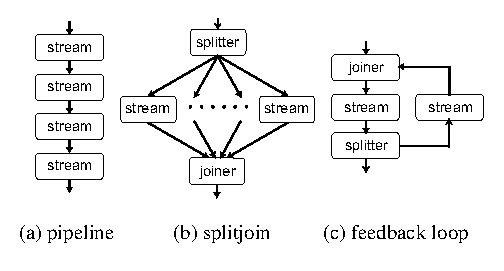
\includegraphics[scale=1, angle=0]{./constructs-eg.eps}
%}
% \vspace{-6pt}
% \nocaptionrule
 \caption{Hierarchical streams in StreamIt.}
 \label{fig:containers}
\end{center}
\end{figure}

\begin{figure}[t]
\begin{center}
\vspace{-12pt}
% \framebox{
 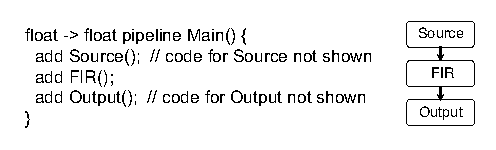
\includegraphics[scale=1, angle=0]{./pipeline-eg.eps}
%}
% \vspace{-6pt}
% \nocaptionrule
 \caption{Example pipeline with FIR filter.}
 \label{fig:pipeline}
%\vspace{-18pt}
\end{center}
\end{figure}

In StreamIt, the
application developer focuses on the hierarchical assembly of the
stream graph and its communication topology, rather than on the 
explicit management of the data buffers between filters.
StreamIt provides three hierarchical structures for composing filters
into larger stream graphs (see Figure~\ref{fig:containers}). The 
{\it pipeline} construct composes streams in sequence, with the output
of one connected to the input of the next.   An example of a pipeline
appears in Figure~\ref{fig:pipeline}.

The {\it splitjoin} construct distributes data to a set of parallel
streams, which are then joined together in a round robin fashion.  In
a splitjoin, the {\it splitter} performs the data scattering, and the
{\it joiner} performs the gathering. A splitter is a specialized
filter with a single input and  multiple output channels. On 
every execution step, it can distribute its output to any one of
its children in either a {\it duplicate} or a {\it roundrobin}
manner. For the former, incoming data are replicated to every
sibling connected to the splitter. For the latter, data are scattered
in a round robin manner, with each item sent to exactly one child
stream, in order.  The splitter type and the weights for distributing data to
child streams are declared as part of the syntax (e.g., \texttt{split
duplicate} or \texttt{split roundrobin($w_1,\ldots,w_n$)}). The
splitter counterpart is the joiner. It is a specialized filter with  
multiple input channels but only one output channel. The joiner
gathers data from its predecessors in a round robin manner (declared
as part of the syntax) to produce a single output stream.

StreamIt also provides a {\it feedback loop} construct for introducing
cycles in the graph.

%\section{Execution Model}
%\label{sec:execmodel}

%% A StreamIt program is represented by a hierarchical graph,
%% where the leaf nodes are filters, splitters, and joiners, and
%% the composite nodes are pipelines, splitjoins, and
%% feedback-loops. Edges in the graph represent data channels, which 
%% operate as FIFO queues.
\paragraph*{Execution Model}
As noted earlier, an actor (i.e., a filter, splitter, or joiner)
executes whenever there are enough data items on its input 
tape. In StreamIt, actors have  two epochs
of execution: one for initialization, and one for the {\it steady
state}. The initialization primes the input tapes to allow filters with
peeking to execute the very first instance of their work functions.
%%initialization in this setting is similar to the prologue stage in
%%software pipelining. 
A steady state is an execution that does not change the
buffering in the channels: the number of items on each channel
after the execution is the same as it was before the execution. 
Every valid stream graph has a steady state~\cite{LM87-i}, and within
a steady state, there are often many possibilities for interleaving
actor executions. 
%% The steady state schedule has the property that
%% the amount of data buffered between any two actors does not change
%% before and after the actor executions.
\begin{figure}[t]
\begin{center}
%%\vspace{-24pt}
%\vspace{24pt}
 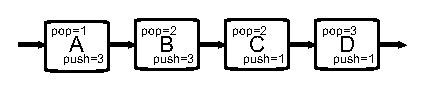
\includegraphics[scale=1, angle=0]{./pipe-with-rates.eps}
%\vspace{-6pt}
% \nocaptionrule
 \caption{Example pipeline.}
 \label{fig:pipe-with-rates}
\end{center}
%\vspace{-12pt}
\end{figure}
An example of a steady state for the pipeline in
Figure~\ref{fig:pipe-with-rates} requires filter \texttt{A} to fire
4 times, \texttt{B} 6 times, \texttt{C} 9 times, and
\texttt{D} 3 times. 
% Because in StreamIt the filters are
% independent (i.e., they do not share state), they can execute
% concurently. In a uniprocessor setting (which is what we use for our
% evaluation), we can only run one filter at time. Therefore, 
% The data generated by one actor are buffered (cached) until they are
% consumed.

\paragraph*{Compilation Process}
The StreamIt compiler derives the initialization and steady state
schedules~\cite{karczma-lctes03} and outputs a C program that includes
the initialization and work functions, as well as a driver to execute
each of the two schedules. Our compilation process allows the StreamIt
compiler to focus on high level optimizations, and relies on existing
compilers to perform machine-specific optimizations such as register
allocation, instruction scheduling, and 
code generation---this two step approach affords us a
great deal of portability (e.g., code generated from the StreamIt
compiler is compiled and run on three different machines as reported
in Section~\ref{sec:evaluation}).

%% For example, referring to
%% Figure~\ref{fig:pipe-with-rates}, the compiler generates the following
%% sample code for running the steady state schedule:
%% %\begin{scriptsize}
%% \begin{verbatim}
%% run_steady_state() {
%%   for (i = 0; i < 4; i++) A_work();
%%   for (i = 0; i < 6; i++) B_work();
%%   for (i = 0; i < 9; i++) C_work();
%%   for (i = 0; i < 3; i++) D_work();
%% }
%% \end{verbatim}
%% %\end{scriptsize}
%% To execute the program, the steady state is wrapped with
%% another loop that invokes the steady state a designated number of
%% times. Preceding the state steady, a similar initialization schedule
%% is run to prime the data buffers.
%, and following the steady state, an
%epilogue is run to drain the buffers as necessary.

%% \begin{figure}[t]
%% \begin{center}
%% \vspace{-12pt}
%%  \psfig{figure=ssi.eps,width=3in}
%%  \vspace{-6pt}
%%  \caption{Instruction size (in bytes along the y-axis) per filter
%%  (x-axis) occurring in a steady state execution of FFT.}
%%  \label{fig:ssi-single}
%% \vspace{-18pt}
%% \end{center}
%% \end{figure}

\section{Precise Event Handling}
\label{sec:language}

In this section we describe how $\sdep$ information can be
incorporated into the semantics of a language feature that provides
precise delivery of control messages in stream programs.  Our goal is
to improve performance as well as programmer productivity.

The Synchronous Dataflow (SDF) domain is well-suited for applications
that have regular, high-bandwidth communication patterns.  However, in
realistic streaming applications there are also irregular,
low-bandwidth control messages that are used to adjust parameters in
various parts of the stream.  For example, a downstream actor might
detect a high signal-to-noise ratio and send a message to the
communications frontend to increase the amplification.  Or, an actor
at the top of the stream graph might detect an invalid checksum for a
packet, and send a message downstream to invalidate the effects of
what has been processed.  Other examples of control messages include:
periodic channel characterization; adaptive beamforming; initiating a
handoff ({\it e.g.,} to a new network protocol); marking the end of a
large data segment; and responding to user inputs, environmental
conditions, or runtime exceptions.

Generally speaking, control messages are sent at infrequent and
irregular intervals; however, once they are generated they might be
tightly constrained with respect to their delivery.  For example, the
message invalidating the effects of a given packet has to be delivered
exactly in sync with the front of the packet itself; otherwise, valid
data will be lost or invalid data will be allowed to pass.

\subsection{Teleport Messaging}
\label{sec:teleport}

Teleport messaging is a language construct that makes use of $\sdep$
to achieve precise timing of control messages.  It is included as part
of the StreamIt language~\cite{streamitcc}.  This section describes
the semantics of teleport messaging; the next section compares it
against other means of implementing messages for a frequency hopping
radio application.

In StreamIt, there are two distinct kinds of communication between
filters during steady state execution: 1) high-bandwidth dataflow over
the FIFO channels in the graph, and 2) low-bandwidth messaging between
pairs of filters\footnote{\small Messaging is possible whenever there
is a downstream path from either filter to the other.  Filters running
in parallel cannot send messages.}.  In order for filter $A$ to send a
message to filter $B$, the following steps need to be taken:
\begin{itemize}

\item $B$ declares a message handler that is invoked when a
message arrives.  For example:
{\small
\begin{verbatim}
handler increaseGain(float amount) {
  this.gain += amount;
}
\end{verbatim}
}
Message handlers are akin to normal functions, except that they
cannot access the input/output channels and they do not return values.

\item A parent stream containing $A$ and $B$ declares a variable
of type {\tt portal<} $T_B$ {\tt >} that can forward messages to
any actor of type $T_B$.  The parent adds $B$ to the portal and passes
the portal to $A$ during initialization.

\item To send a message, $A$ invokes the handler method on the portal
from within its steady state work function. The handler invocation
includes a range of latencies specifying when the message should be
delivered: {\small
\begin{verbatim}
work pop 1 {
  float val = pop();
  if (val < THRESHOLD) {
    portalToB.increaseGain(0.1) [2:3];
  }
}
\end{verbatim}}
This code sends an {\tt increaseGain} message to {\tt portalToB} with
minimum latency 2 and maximum latency 3.

\end{itemize}
The most interesting aspect of teleport messaging are the semantics
for the message latency.  Because there are many legal orderings of
actor executions, there does not exist a notion of ``global time'' in
a stream graph.  The only common frame of reference between
concurrently executing actors is the series of data items that is
passed between them.  The $\sdep$ function captures the data
dependences in the graph and provides a natural means of defining a
rendezvous point between two actors.

Intuitively, the message semantics can be thought of in terms of
attaching tags to data items.  If $A$ sends a message to downstream
filter $B$ with a latency $k$, then this could be implemented by
tagging the items that $A$ outputs $k$ iterations later.  These tags
propagate through the stream graph; whenever an actor inputs an item
that is tagged, all of its subsequent outputs are tagged.  Then, the
message handler of $B$ is invoked immediately before the first
invocation of $B$ that inputs a tagged item.  In this sense, the
message has the semantics of traveling ``with the data'' through the
stream graph, even though it does not have to be implemented this way.

The intuition for upstream messages is similar.  Consider that $B$ is
sending a message with latency $k$ to upstream actor $A$ in the stream
graph.  This means that $A$ will receive the message immediately
before the last invocation of its work function that produces an item
affecting the output of $B$'s $k$th firing, counting the current
firing as 0.  As before, we can also think of this in terms of $A$
tagging items and $B$ observing the tags.  In this case, the latency
constraint says that $B$ must input a tagged item before it finishes
$k$ additional executions.  The message is delivered immediately
before the latest firing in $A$ during which tagging could start
without violating this constraint.

\begin{table*}[t]
\begin{center}
{\small
\begin{tabular}{|r|c|c|} \hline
~ & {\bf Negative latency} & {\bf Positive latency} \\ \hline
{\bf Message travels downstream} & latency in schedule must not be too small & no constraint \\ \hline
{\bf Message travels upstream} & illegal & latency in schedule must not be too big \\ \hline
\end{tabular}}
\caption{\small Scheduling constraints imposed by messages.}
\label{tab:messcons}
\end{center}
\vspace{-12pt}
\end{table*}

The following definition leverages the $\sdep$ formalism to give a
precise meaning to message timing.

\begin{definition}(Message delivery)
Consider that $S$ sends a message to receiver $R$ with latency range
$[k_1:k_2]$ and that the message is sent during the $n$th invocation
of $S$'s work function.  Then the message handler can be invoked in
$R$ immediately before its work function has fired ${\cal M}(S, R,
k_1, k_2, n)$ times, where ${\cal M}$ is constrained as follows.

There are two cases\footnote{In a feedback path, both cases might apply.  In this event, we assume the message is being sent upstream.}:
\begin{enumerate}

\item There is a path in the stream graph from $S$ to $R$.  Then
${\cal M}$ obeys the following constraints:
\[
\begin{array}{l}
\sdepf{S}{R}({\cal M}(S, R, k_1, k_2, n)) \ge n+k_1\\
\sdepf{S}{R}({\cal M}(S, R, k_1, k_2, n)) \le n+k_2
\end{array}
\]

\item There is a path in the stream graph from $R$ to $S$.  Then
${\cal M}$ obeys the following constraints:
\[
\begin{array}{l}
{\cal M}(S, R, k_1, k_2, n) \ge \sdepf{R}{S}(n + k_1)\\
{\cal M}(S, R, k_1, k_2, n) \le \sdepf{R}{S}(n + k_2)
\end{array}
\]
\end{enumerate}
\end{definition}

It is instructive to note that messaging can place constraints on the
execution schedule.  The different categories of constraints are
illustrated in Figure~\ref{tab:messcons}.  A negative-latency
downstream message has the effect of synchronizing the arrival of the
message with some data that was previously output by the sender ({\it
e.g.,} for the checksum example mentioned earlier).  The latency
requires the downstream actor not to execute too far ahead, or else it
might process the data before the message arrives.  This translates to
a constraint on the minimum latency between the sender and receiver
actors in the schedule of the program.

Similarly, a positive latency upstream message places a constraint on
the maximum latency between the sender and receiver.  Again the
receiver must be throttled so that it does not get too far ahead
before the message arrives.

An upstream message with negative latency is impossible to deliver,
because the data dependences imply that the target iteration has
already passed when the message was sent.  Conversely, a downstream
message with positive latency imposes no constraint on the schedule,
as the sender has not yet produced the data that is synchronized with
the message.

%\begin{figure}[t]
\begin{center}
\psfig{figure=constrained-example.eps,height=1.5in}
\caption{{\small Example of construction of a constrained schedule. The $\sdepf{R}{S}$ function for filters $R$ and $S$ is given in Table \ref{tab:sdepconst}. The blob between filters $R$ and $S$ illustrates other possible stream elements. $R$ sends a message to $S$ with latency $[1,2]$. Executions of the blob are ommitted, it is assumed that at the point $S$ executes, the blob has drained data provided by $R$.}}
\end{center}
\vspace{-12pt}
\label{fig:sdepconst}
\end{figure}

\begin{table*}[t]
{\small
\begin{tabular}{|c|c|} \hline
{\bf $sdepf{R}{S}$} & {\bf Execs of S} \\ \hline
$9n+2$ & $8n+1$ \\ \hline
$9n+3$ & $8n+2$ \\ \hline
$9n+5$ & $8n+3$ \\ \hline
$9n+5$ & $8n+4$ \\ \hline
$9n+6$ & $8n+5$ \\ \hline
$9n+8$ & $8n+6$ \\ \hline
$9n+9$ & $8n+7$ \\ \hline
$9n+9$ & $8n+8$ \\ \hline
\end{tabular}}
\caption{\small $sdepf{R}{S}$ function for example in Figure \ref{fig:sdepconst}. This particular $\sdep$ function was obtained by setting $push_R=2$, $pop_S=3$ and making the blob between $R$ and $S$ into a filter that pops 3 and pushes 4 every iteration of its work function. No initialization due to peeking is necessary in this example.}
\label{tab:sdepconst}
\end{table*}


Explanation of working of the example:

The example in Figure \ref{fig:sdepconst} illustrates scheduling of a single constraint. The constraint is a message sent upstream with latency $[1,2]$. The resulting schedule consists of two parts, an initialization schedule and a steady state schedule. The initialization schedule is necessary to initialize the constraint, to ensure that the steady schedule can be executed repeatedly forever. Notation used here is: $lastReceived$ denotes the execution of S which sent the last message to be received by R; $n_S$ indicates number of executions of $S$ and $n_R$ indicates number of executions of $R$.

Initialization schedule is computed by executing R $SDEP(minLatency)-1$ number of times, and executing S as many times as possible, given data provided by R. This assures that when the steady schedule starts, all executions of filters will contribute to new message sending and receiving, thus allowing the steady state schedule to execute forever. The initialization schedule does not need to send or receive messages here.

The steady state schedule is computed by executing the receiver R as far as possible without going beyond the boundary of beeing able to receive message sent by S on execution $lastReceived+1$ (indicated by "Oldest msg to receive" in the figure). Now the sender S is executed as many times as possible, given data provided by R. Now S can receive messages sent by S in its executions $[lastReceived+1 ... \min(n_S, $"Newest msg to receive"$)]$.

"Oldest msg to receive" is equal to $iSDEP(n_R)-maxLatency$. "Newest msg to receive" is equal to $m-minLatency$ with $m$ being the greatest integer such that $SDEP(m) \le n_R$.


\subsection{Case Study}

To illustrate the pros and cons of teleport messaging, we implemented
a spread-spectrum frequency hopping radio frontend~\cite{harada02} as
shown in Figure~\ref{fig:fhr-streamit}.  A frequency hopping radio is
one in which the receiver switches between a set of known frequencies
whenever it detects certain tones from the transmitter.  The frequency
hopping is a good match for control messages because the hopping
interval is dynamic (based on the data in the stream); it spans a
large section of the stream graph (there is an FFT between the
demodulator and the hop detector); and it requires precise delivery of
messages.  The delivery must be precise both to meet real-time
requirements (as the transceiver will leave the current frequency
soon), and to ensure that the message falls at a logical packet
boundary; if the frequency change is out of sync with the Fast Fourier
Transform (FFT) stage, then the FFT will muddle the spectrum of the
old and new frequency bands.

A StreamIt version of the radio frontend with teleport messaging
appears in Figure~\ref{fig:freq1}.  The Freq\_Hopping\_Radio pipeline
creates a portal and adds the RFtoIF actor as a receiver.  The portal
is passed to the Check\_Freq\_Hop stage, where four parallel detectors
send messages into the portal if they detect a hop to the frequency
they are monitoring.  The messages are sent with a latency of 4 to
ensure a timely transition.  To make sense of the latency, note that
$\sdepf{RFtoIF}{D}(n) = 64*n$ for each of the detector actors $D$.
This comes about because the FFT stage consumes and produces 64 items;
each detector fires once per set of outputs from the FFT, but RFtoIF
fires 64 times to fill the FFT input.  Because of this $\sdep$
relationship, messages sent from the detectors to RFtoIF are
guaranteed to arrive only at iterations that are a multiple of 64.
This satisfies the design criterion that a given FFT stage will not
operate on data that was demodulated at two separate frequencies.

Another version of the frequency hopping radio appears in
Figures~\ref{fig:fhr-manual} and~\ref{fig:freq2}.  This version is
functionally equivalent to the first, except that the control messages
are implemented manually by embedding them in the data stream and
introducing a feedback loop.  Because the number of items transfered
around the loop must be constant from one iteration to the next, a
data item is sent whether or not there is a message as part of the
algorithm; a special value of 0 represents that there is not a message
on the given iteration (in some other programs, if a special value is
not available, a structure may be passed through the stream with a
boolean flag indicating whether or not a message is present).  The
RFtoIF filter checks the values from the loop on every iteration and
processes them as a message if they are non-zero.  The I/O rate of the
RFtoIF filter has been scaled up to ensure that the messaging
information is received at intervals of 64 iterations (as in the
version with portals).  To achieve the desired messaging latency, a
number of items are enqueued on the feedback path prior to execution.

Yet another way to approximate the behavior of messaging is with a
direct function call from the detector to the RFtoIF stage.  (Though
such a call is disallowed in StreamIt, it could be an option in a
different programming model.)  While this approach is simple, it does
not have any timing guarantees.  There is no way for the sender to
know when in the course of the target's execution the message will be
received.  This could cause problems both for algorithm development
and for reliability / predictability of software.

\vspace{12pt}
\subsection{Discussion}

We believe that teleport messaging offers several benefits compared to
a manual implementation of equivalent functionality.  While embedding
messages in the data stream is equally precise, this involves several
tedious and error-prone changes, not only to the stream graph but also
to the steady state execution code within the actors.  In particular,
the manual derivation of the loop delay, adjustment of the actor I/O
rates, and implicit interleaving of data items with control messages
has a negative impact on the readability and maintainability of the
code.  Teleport messaging provides the same level of precision, but
with the simplicity of a method call.

Teleport messaging also has advantages from a compiler standpoint.  By
separating the data-intensive code from the control-oriented code, the
common case of the steady state actor execution is not sacrificed for
the uncommon case of message processing.  There are no ``dummy items''
serving as placeholders in the static-rate channels.  In addition, by
exposing the message latency as part of the language, the compiler can
infer the true dependences between filter firings and reorder the
execution so long as the message constraints are respected.  The
actual message delivery can be implemented in the most efficient way
for the given architecture.

\clearpage
\begin{figure}[t]
\psfig{figure=fhr-streamit.eps,width=3.5in}
\caption{\small Stream graph of frequency-hopping radio with teleport messaging.  
A portal delivers point-to-point latency-constrained messages from the
detectors to the RFtoIF stage.
\protect\label{fig:fhr-streamit}}
\end{figure}

\begin{figure}[t]
\psfig{figure=code-freq1.eps,width=3.5in}
\caption{\small Frequency hopping radio with teleport messaging.
Arrows depict the path of messages from the sender to the receiver,
via a portal declared in the top-level stream.
\protect\label{fig:freq1}}
\end{figure}

\clearpage
\begin{figure}[t]
\psfig{figure=fhr-feedback.eps,width=3.5in}
\caption{\small Stream graph of frequency-hopping radio with control
messages implemented manually.  A feedback loop connects the detectors
with the RFtoIF stage, and an item is sent on every invocation to
indicate whether or not a message is present.  The latency and
periodicity of message delivery are governed by the data rates and the
number of items on the feedback
path. \protect\label{fig:fhr-manual}}
\end{figure}

\begin{figure}[t]
\psfig{figure=code-freq2.eps,width=3.5in}
\caption{\small Frequency hopping radio with manual feedback loop for
event handling.  Lines that differ from Figure~\ref{fig:freq1} are
marked with an asterisk. \protect\label{fig:freq2}}
\end{figure}
\clearpage


A final benefit of teleport messaging is the clean interface provided
by the portals.  Since a portal can have multiple receivers, it is
straightforward to send a message that is delivered synchronously to
two actors in parallel streams.  For example, consider a vocoder (an
encoder for voice signals) that is separately manipulating the
magnitude and phase components of a signal.  If something triggers an
adjustment to the speech transformation ({\it e.g.,} the speaker
requests a change of pitch) then the mask needs to be updated at the
same time relative to data in both parallel streams.  A portal that
contains both components seamlessly provides this functionality.
Finally, portals are useful as an external programming interface; an
application can export a portal based on an interface type without
exposing the underlying actor implementation.


\startchapter{Optimizing Stream Programs}
\label{chap:optimizing}

This chapter validates the premise that stream programming enables new
and powerful optimiations that are outside the reach of a traditional
compiler.  We highlight three projects in the StreamIt group:

\begin{enumerate}

\item {\it Parallelization.}  We demonstrate an end-to-end stream 
compiler that attains robust multicore performance in the face of
varying application characteristics.  As benchmarks exhibit different
amounts of task, data, and pipeline parallelism, we exploit all types
of parallelism in a unified manner in order to achieve this
generality.  Our compiler, which maps from the StreamIt language to
the 16-core Raw architecture, attains an 11x mean speedup and an 18x
maximum speedup over a single-core baseline.  {\it Project leader:}
Michael Gordon~\cite{gordon06asplos}.

\item {\it Optimizing Linear Computations}.  We demonstrate that 
several algorithmic transformations, traditionally hand-tuned by DSP
experts, can be completely automated by the compiler.  We focus on
linear filters, where each output is an affine combination of the
inputs.  We present several optimizations of linear filters, including
algebraic simplification of adjacent filters and automatic translation
to the frequency domain.  These transformations offer an average
speedup of 5.5x and a maximum speedup of 8.0x over unoptimized
StreamIt on a Pentium~4.  {\it Project leaders:} Andrew
Lamb~\cite{lamb:pldi:2003,lamb-thesis} and Sitij
Agrawal~\cite{agrawal:cases:2005,agrawal-thesis}.

\item {\it Cache Optimizations}.   We formulate a set of cache aware 
optimizations that automatically improve instruction and data
locality.  We highlight two techniques: 1) cache aware fusion, which
combines adjacent filters while respecting instruction cache
constraints, and 2) cache aware scaling, which improves instruction
locality while respecting data cache constraints.  Our implementation
of cache aware optimizations in the StreamIt compiler yields a 3.49x
average speedup and an 88x maximum speedup over unoptimized StreamIt
on a StrongARM 1110 processor.  {\it Project leader:} Janis
Sermulins~\cite{sermulins:lctes:2005,sermulins-thesis}.

\end{enumerate}

While the author contributed to each of these projects, they are the
full-time focus of other individuals and also appear (or will appear)
in their theses.  Unlike the other chapters in this thesis, our
treatment does not aim to be comprehensive.  For more details, please
consult the papers referenced above.

\section{Parallelization}

%% Our compiler relies on two new techniques.  {\it Coarse-grained data
%% parallelism} increases the granularity of data-parallel streams to
%% match the coarse-grained nature of multicores.  It is analogous to
%% fusion of DOALL loops in the scientific domain.  {\it Coarse-grained
%% software pipelining} applies traditional instruction-scheduling
%% techniques at the level of coarse-grained actors, offering a new level
%% of scheduling freedom for stream programs.  The techniques are
%% complementary and are best when applied together.

%%%%%%%%%%%%%%%%%%%%%%%%%%%%%%%%%%%%%%%%%%%%%%%%%%%%%%%%%%

%% The first technique exploits {\it coarse-grained data parallelism} by
%% duplicating data-parallel sections across cores.  While traditional
%% data parallelism incurs excessive communication and synchronization
%% costs on multicores, our technique utilizes a program analysis to
%% coarsen the granularity of data-parallel actors and duplicate them the
%% minimum number of times needed.  The second technique, {\it
%% coarse-grained software pipelining}, leverages powerful properties of
%% the stream programming model to apply traditional
%% instruction-scheduling techniques at the level of coarse-grained
%% actors.  This increases scheduling freedom and extracts valuable
%% pipeline parallelism from the application.

%%%%%%%%%%%%%%%%%%%%%%%%%%%%%%%%%%%%%%%%%%%%%%%%%%%%%%%%%%

%% In this paper, we describe two new techniques for mapping stream
%% programs to multicores.  The first technique exploits {\it
%% coarse-grained data parallelism} by duplicating data-parallel sections
%% across cores.  While traditional data parallelism incurs excessive
%% communication and synchronization costs on multicores, our technique
%% utilizes a program analysis to coarsen the granularity of
%% data-parallel actors and duplicate them the minimum number of times
%% needed.  The second technique, {\it coarse-grained software
%% pipelining}, leverages powerful properties of the stream programming
%% model to apply traditional instruction-scheduling techniques at the
%% level of coarse-grained actors.  This increases scheduling freedom and
%% extracts valuable pipeline parallelism from the application.

%% We have implemented these techniques in the StreamIt compiler,
%% targeting the 16-core Raw architecture.  Coarse-grained data
%% parallelism offers a 9.9x mean speedup over a single-core baseline,
%% while coarse-grained software pipelining offers a 7.7x speedup.
%% Combining the techniques yields the best results, achieving a 11.2x
%% speedup over a single core and 1.84x over our previous work.

Despite the abundance of parallelism in stream programs, it is
nonetheless a challenging problem to obtain an efficient mapping to a
multicore architecture.  Often the gains from parallel execution can
be overshadowed by the costs of communication and synchronization.  In
addition, not all parallelism has equal benefits, as there is
sometimes a critical path that can only be reduced by running certain
actors in parallel.  Due to these concerns, it is critical to leverage
the right combination of task, data, and pipeline parallelism while
avoiding the hazards associated with each.

\begin{figure}[t]
\centering
\psfig{figure=parallelism.eps,width=2.1in}
\caption[Types of parallelism in stream programs]{Types of parallelism
  in stream programs.  Task parallelism exists between filters in a
  common splitjoin; pipeline parallelism exists between filters in a
  producer/consumer relationship; and data parallelism exists between
  separate instances of a stateless
  filter.\protect\label{fig:parallelism}}
\end{figure}

Task parallelism refers to pairs of actors that are on different
parallel branches of the original stream graph, as written by the
programmer.  That is, the output of each actor never reaches the input
of the other (see Figure~\ref{fig:parallelism}).  In stream
programs, task parallelism reflects logical parallelism in the
underlying algorithm.  It is easy to exploit by mapping each task to
an independent processor and splitting or joining the data stream at
the endpoints.  The hazards associated with task parallelism are the
communication and synchronization associated with the splits and
joins.  Also, as the granularity of task parallelism depends on the
application (and the programmer), it is not sufficient as the only
source of parallelism.

Data parallelism refers to any actor that has no dependences between
one execution and the next.  Such ``stateless'' actors\footnote{A
  stateless actor may still have read-only state.}  offer unlimited
data parallelism, as different instances of the actor can be spread
across any number of computation units.  However, while data
parallelism is well-suited to vector machines, on coarse-grained
multicore architectures it can introduce excessive communication
overhead.  Previous data-parallel streaming architectures have focused
on designing a special memory hierarchy to support this
communication~\cite{imagine03ieee}.  However, data parallelism has the
hazard of increasing buffering and latency, and the limitation of
being unable to parallelize actors with state.

Pipeline parallelism applies to chains of producers and consumers that
are directly connected in the stream graph.  In our previous
work~\cite{streamit-asplos}, we exploited pipeline parallelism by
mapping clusters of producers and consumers to different cores and
using an on-chip network for direct communication between actors.
Compared to data parallelism, this approach offers reduced latency,
reduced buffering, and good locality.  It does not introduce any
extraneous communication, and it provides the ability to execute any
pair of stateful actors in parallel.  However, this form of pipelining
introduces extra synchronization, as producers and consumers must stay
tightly coupled in their execution.  In addition, effective load
balancing is critical, as the throughput of the stream graph is equal
to the minimum throughput across all of the processors.

In this section, we describe a robust compiler system that leverages
the right combination of task, data, and pipeline parallelism to
achieve good multicore performance across a wide range of input
programs.  Because no single type of parallelism is a perfect fit for
all situations, a unified approach is needed to obtain consistent
results.  Using StreamIt as our input and targeting the 16-core Raw
architecture, our compiler demonstrates a mean speedup of 11.2x over a
single-core baseline.  This also represents a 1.84x improvement over
our original approach~\cite{streamit-asplos}.

\subsection*{Parallelization Algorithm}

\begin{figure}[t]

\begin{minipage}{0.3\textwidth}
\centering
\psfig{figure=filterbank.eps,width=1.6in}
\end{minipage}
\hspace{0.1in}
\begin{minipage}{0.3\textwidth}
\centering
\psfig{figure=filterbank-fine.eps,width=2.2in}
\end{minipage}
\hspace{0.4in}
\begin{minipage}{0.3\textwidth}
\centering
\psfig{figure=filterbank-coarse.eps,width=1.6in}
\end{minipage}

~ \\
\begin{minipage}{0.3\textwidth}
\centering
\mbox{{\small (a) Original}}
\end{minipage}
\hspace{0.1in}
\begin{minipage}{0.3\textwidth}
\mbox{{\small (b) Fine-grained data parallelism}}
\end{minipage}
\hspace{0.4in}
\begin{minipage}{0.3\textwidth}
\hspace{-14pt}\mbox{{\small (c) Coarse-grained data parallelism}}
\end{minipage}

\centering
\caption[Exploiting data parallelism in the FilterBank
  benchmark]{Mapping a simplified version of the FilterBank benchmark
  for execution on four cores.  The original stream graph is shown in
  (a), while a conventional mapping is shown in (b).  Our technique
  coarsens the graph and introduces the minimal parallelism needed, as
  shown in (c).\protect\label{fig:filterbank}}

\end{figure}

We illustrate our technique by way of an example: we discuss how to
map a simplified version of our FilterBank benchmark (see
Figure~\ref{fig:filterbank}a) to a four-core machine.  The complete
details of our algorithm are available
elsewhere~\cite{gordon06asplos}.

\paragraph*{Previous Practice: Fine-Grained Data Parallelism}  Perhaps 
the most common approach to parallelization is to identify loops that
can be run in a data-parallel (DOALL) style.  Such loops can be
annotated by the programmer using OpenMP; they are also the most
common parallelization target of production compilers.  For example,
the Intel C Compiler includes an optional flag to detect and
parallelize data-parallel loops.  In the case of FilterBank, this may
seem like a promising approach, as all the filters are stateless and
the implicit loops surrounding them can be run in a data-parallel
manner.  Figure~\ref{fig:filterbank}b illustrates such a mapping.

Unfortunately, on a coarse-grained multicore architecture, it is
hardly profitable to parallelize each individual filter due to the
communication and synchronization overheads incurred.  When we target
the 16-core Raw architecture, this approach offers only a 1.4x mean
speedup over a single core.  This represents an upper bound on the
speedups attainable using standard techniques.  In practice, for
reasons explained in Section~\ref{sec:filters}, a production C
compiler would achieve even smaller speedups due to the inherent
difficulties of proving that filters are data-parallel.

\paragraph*{First Innovation: Coarse-Grained Data Parallelism}  The
overheads of fine-grained data parallelism can be drastically reduced
by performing two novel transformations.  First, the granularity of
the stream graph is coarsened via filter {\it fusion}, a
transformation in which two neighboring filters are statically
scheduled and inlined into a single
filter~\cite{streamit-asplos,sermulins:lctes:2005}.  We fuse
neighboring stateless filters as much as possible so long as the
resulting filter remains stateless, ensuring that it is still amenable
to data parallelism.

Second, we data-parallelize the coarsened filters, but only by the
amount necessary to complement existing task parallelism in the stream
graph.  That is, for filters that are already embedded in a splitjoin,
we parallelize each filter so that the total splitjoin width covers
all of the cores, rather than data-parallelizing each branch of the
splitjoin to cover all of the cores.  By reducing the width of the
scatter and gather stages, we reduce the communication and
synchronization overhead incurred by data parallelism.

Figure~\ref{fig:filterbank}c shows an example of our
transformations on the FilterBank benchmark.  The coarsening stage
fuses all of the pipelines together with the exception of the BandStop
filter, which is not fused because it performs peeking on its input
channel.  Communication with peeking represents a case where some data
items are reused between successive firings of a filter, which would
translate to internal state if the buffer were to be inlined into a
fused filter.  Following coarsening, the parallelization stage
replicates the Adder filter across all four of the target cores.
However, the other filters are split only two ways, due to the
presence of task parallelism between alternate branches of the
splitjoin.  Applying this strategy across our benchmark suite offers a
speedup of 9.9x relative to a single core.

These transformations are out-of-reach of traditional compilers.  In
an imperative language, the analog of graph coarsening is to
selectively fuse loops so long as no new loop-carried dependences are
introduced.  The analog of task-conscious data parallelism is to
analyze the entire program for other threads that might be running
concurrently, and to introduce only as much parallelism as is needed
to complement the other threads.  We rely on the properties of the
stream programming model to make these transformations tractable.

\begin{figure}[t]
\centering
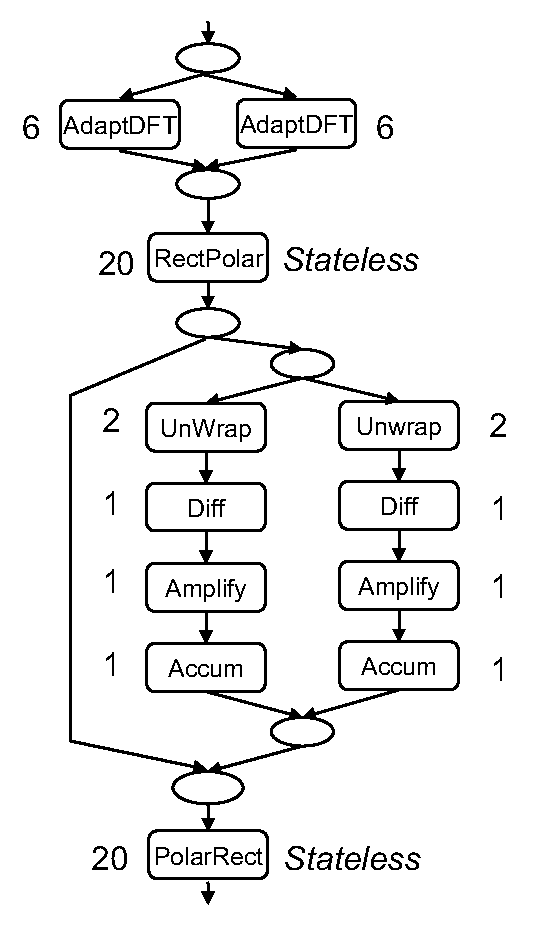
\psfig{file=vocoder.eps,width=2in}
\caption[Simplified subset of the Vocoder benchmark]{Simplified subset
  of the Vocoder benchmark.  Nodes are annotated with the amount of
  work that they perform per steady state.\protect\label{fig:vocoder}}
\end{figure}

\begin{figure}[t]
\centering
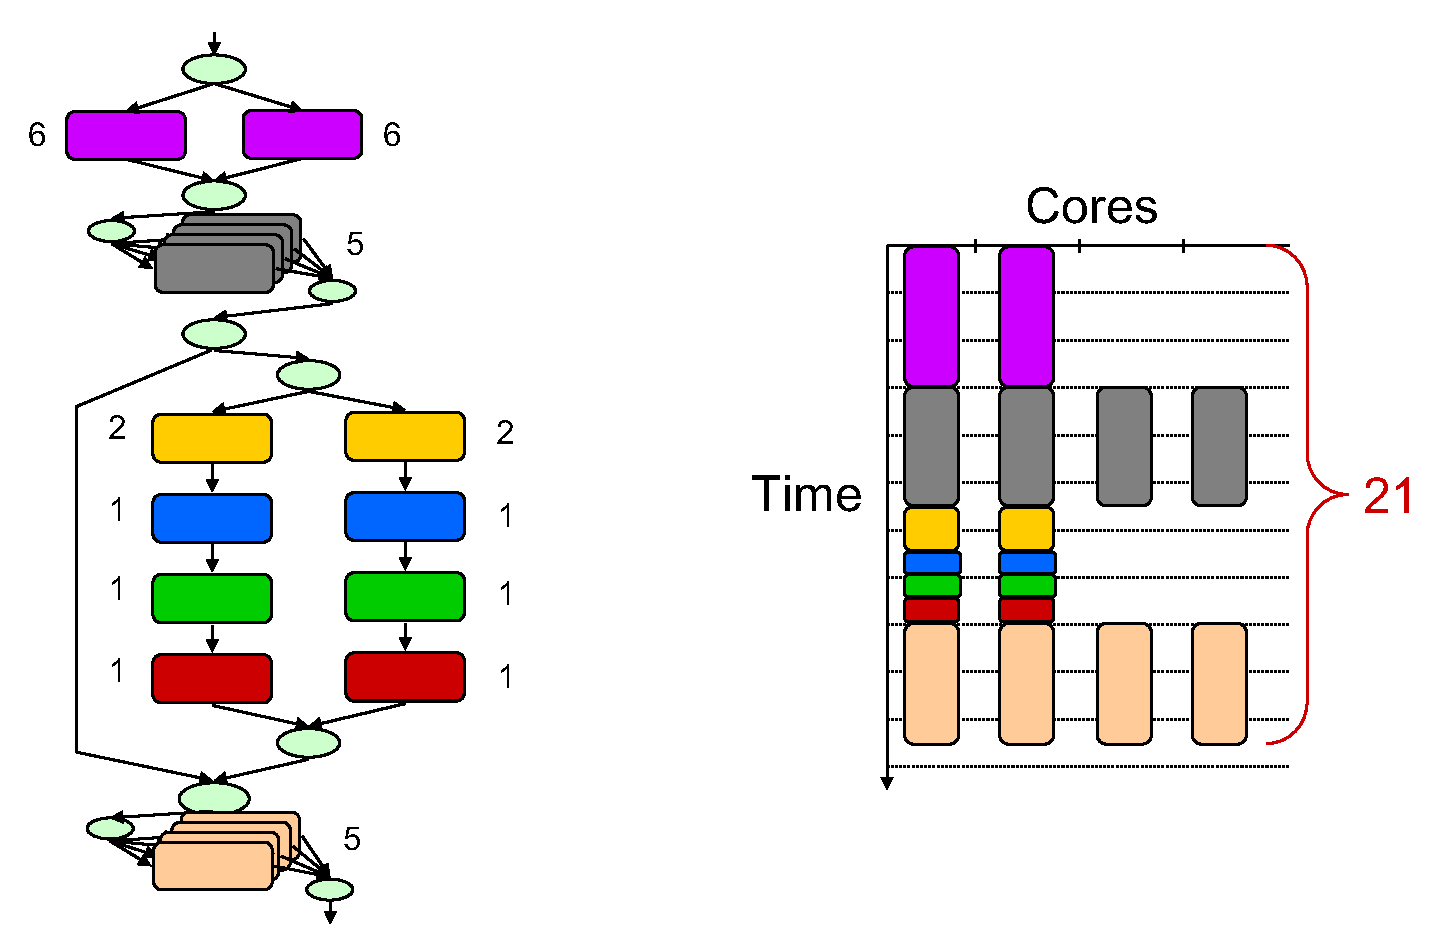
\psfig{file=vocoder-data.eps,width=4.5in}
\caption[Coarse-grained data parallelism applied to
  Vocoder]{Simplified vocoder mapped with data parallelism.  In the
  stream graph (left), stateless nodes are replicated but stateful
  nodes remain untouched.  An execution trace (right) requires 21
  units per steady state.\protect\label{fig:vocoder-data}}
\end{figure}

\begin{figure}[t]
\centering
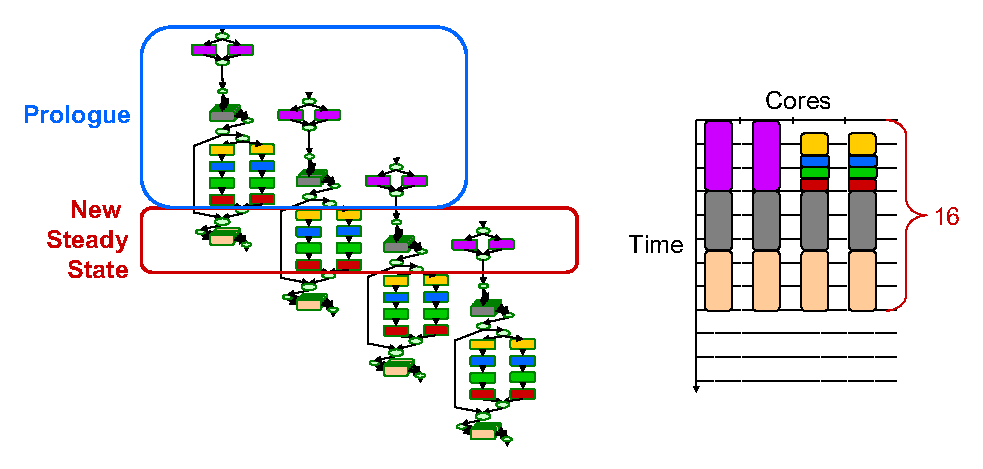
\psfig{file=vocoder-swpipe.eps,width=6in}
\caption[Coarse-grained software pipelining applied to
  Vocoder]{Simplified vocoder mapped with coarse-grained software
  pipelining.  By unrolling multiple executions of the stream graph
  (left), stateful nodes can run in parallel with other nodes during
  the steady state.  An execution trace (right) requires 16 units per
  steady state, an improvement over plain data parallelism.
  \protect\label{fig:vocoder-swpipe}}
\end{figure}

%% \begin{figure}[t]
%% \centering
%% \psfig{figure=asplos06/vocoder.eps,width=4.2in}
%% \vspace{-24pt}
%% \caption{Stream graph for a simplified subset of our Vocoder
%% benchmark.  Following a set of sliding DFTs, the signal is converted
%% to polar coordinates.  Node {\tt S2} sends the magnitude component to
%% the left and the phase component to the right.  In this simplified
%% example, no magnitude adjustment is needed.\label{fig:vocoder}}
%% \vspace{-12pt}
%% \end{figure}

\paragraph*{Second Innovation: Coarse-Grained Software Pipelining} While 
coarse-grained data parallelism is effective for parallelizing
stateless computations, it does nothing to help with computations that
retain state, either within filters or within feedbackloops.  For
example, the Vocoder benchmark (simplified subet shown in
Figure~\ref{fig:vocoder}) contains a significant fraction of stateful
filters.  While two of the filters can be data-parallelized, there
remain large gaps in the execution schedule (see
Figure~\ref{fig:vocoder-data}).

To run stateful computations in parallel with each other, we exploit
pipeline parallelism.  We take the concept of software pipelining,
well-understood in the context of instruction scheduling, and apply it
in the context of an entire stream graph.  As illustrated in
Figure~\ref{fig:vocoder-swpipe}, this technique involves unrolling the
execution of the graph into two stages.  In the first stage, a
prologue schedule establishes buffering in the data channels.  Then,
in the steady state, the filters are decoupled and can execute in any
order, writing intermediate results to the buffers.  Compared to
exploiting only coarse-grained data parallelism, this technique offers
large gains for our stateful benchmarks (1.7x for Vocoder, 1.9x for
Radar).  Together with coarse-grained data parallelism, it offers an
11.2x speedup over a single core across our benchmark suite.

Coarse-grained software pipelining is also beyond the reach of
traditional compilers.  Rather than pipelining individual
instructions, it represents the pipelining of entire procedures.  This
involves reordering large pieces of the program.  The stream
programming model makes such a transformation feasible by exposing the
stable flows of data between long-running actors.

\subsection*{Experimental Evaluation}

%\begin{figure}
%\centering
%\psfig{figure=asplos06/raw-diagram.eps,width=3in}
%\caption{Block diagram of the Raw architecture.
%\protect\label{fig:raw-diagram}}
%\end{figure}

We target the Raw microprocessor~\cite{raw10,raw}, a tiled array of 16
cores with a programmable mesh interconnect.  Though Raw has been
implemented in silicon, we generate results with the btl simulator,
augmented with 16 streaming DRAM controllers (providing enough
bandwidth to saturate both directions of a Raw port).  In this
configuration, one can obtain higher throughput in streaming data from
the off-chip memory than from a core's local data cache.  Thus, our
implementation elects to buffer all streaming data off-chip.  However,
when targeting an architecture with more modest off-chip memory
bandwidth, the stream buffers could reside completely in on-chip
memory.

\begin{figure}[t]
\centering
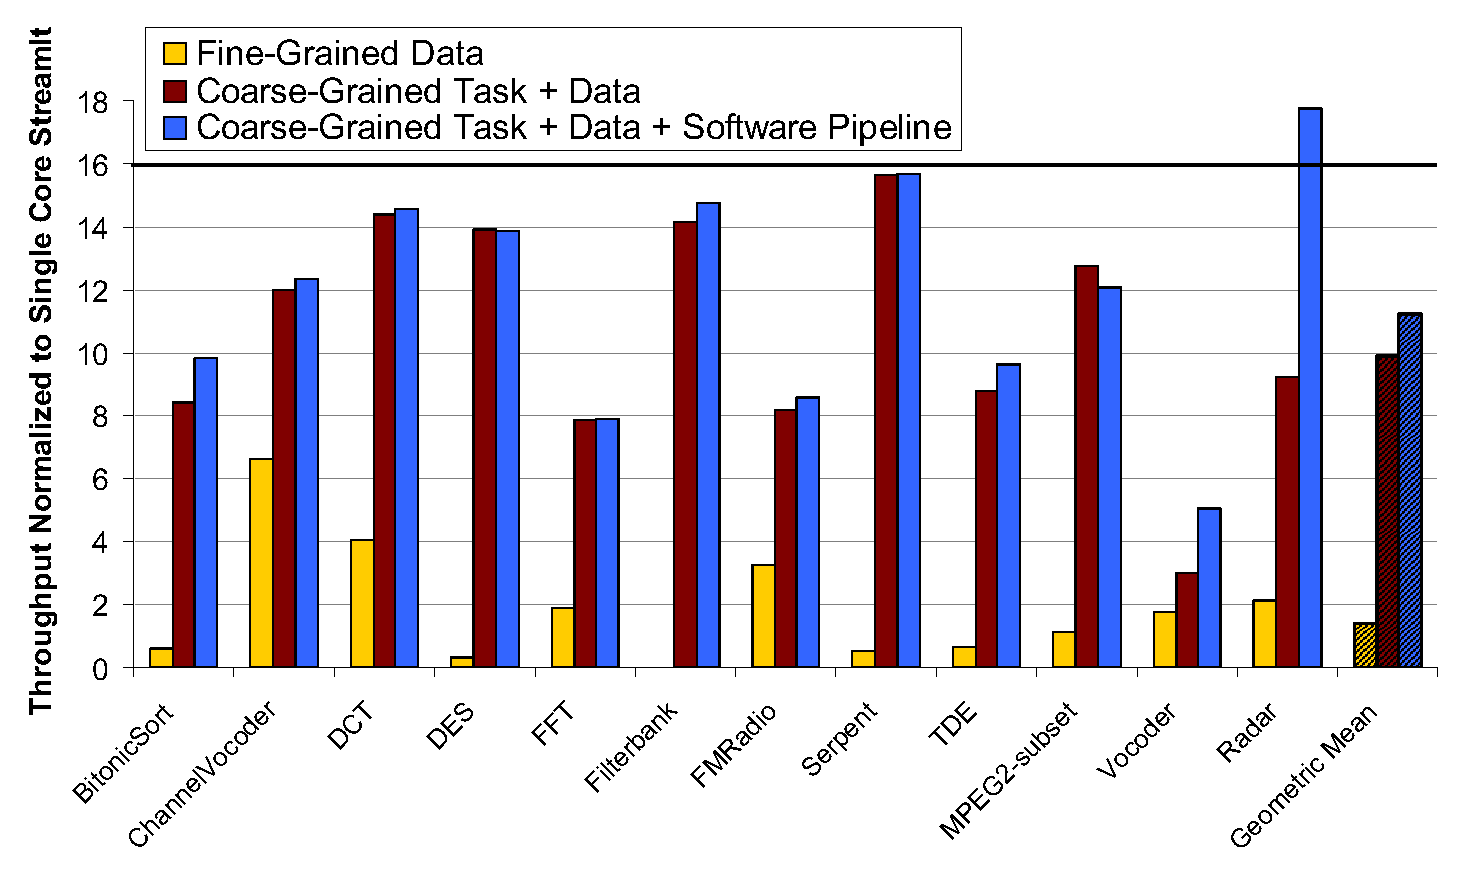
\psfig{file=par-results.eps,width=\textwidth}
\caption[Parallelization results]{Parallelization results on the
  16-core Raw processor.\protect\label{fig:par-results}}
\end{figure}

A summary of our results appears in Figure~\ref{fig:par-results}.  We
show the speedup offered by the three techniques mentioned:
fine-grained data parallelism, the previous standard; coarse-grained
data parallelism, which also leverages the existing task parallelism
in the stream graph; and coarse-grained software pipelining, which
runs as a post-pass to coarse-grained data parallelism.  Our baseline
is StreamIt executing on a single core, which (in the case of Raw) has
been shown to outperform hand-written C implementations on a single
core~\cite{raw_isca}.  While coarse-grained data parallelism performs
well (attaining a mean speedup of 9.9x), the most robust performance
comes by adding coarse-grained software pipelining (which attains a
mean speedup of 11.2x).  As expected, software pipelining mostly
benefits the stateful benchmarks, Vocoder and Radar.  There is a
super-linear speedup in Radar because reordering operations were moved
from the compute core to the network.

%% \begin{figure}[t]
%% \centering
%% \psfig{figure=asplos06/benchchar.eps, width=6.15in}
%% \caption{Benchmark descriptions and characteristics.
%% \protect\label{fig:benchchar}}
%% \end{figure}

%% \begin{figure}[t]
%% \centering
%% \psfig{figure=asplos06/thruput.eps, width=6.1in}
%% \caption{Throughput speedup comparison and Task + Data + Software
%% Pipelining performance results.  \protect\label{fig:thruput}}
%% \end{figure}

%% \begin{figure}[t]
%% \centering
%% \psfig{figure=asplos06/maingraph.eps, width=6.5in}
%% \caption{Task, Task + Data, Task + Software Pipelining, and Task +
%% Data + Software Pipelining normalized to single core.
%% \protect\label{fig:main_comp}}
%% \end{figure}

%% \begin{figure}[t]
%% \centering
%% \psfig{figure=asplos06/fine_data.eps, width=4.5in}
%% \caption{Fine-Grained Data Parallelism normalized to single core.
%% \protect\label{fig:fine_data}}
%% \end{figure}

%% \begin{figure}[t]
%% \centering
%% \psfig{figure=asplos06/vs_space_graph.eps, width=4.5in}
%% \caption{Task + Data + Software Pipelining normalized to Hardware Pipelining.
%% \protect\label{fig:vs-space}}
%% \end{figure}

\section{Optimizing Linear Computations}

The design flow for digital signal processing applications typically
contains three steps.  First, application designers specify a block
diagram of the computation, drawing on rich software libraries to
prototype its behavior in an environment such as MATLAB.  Once the the
functionality has been fixed, the second step is performed by digital
signal processing (DSP) experts, who inspect the global structure of
application and perform many domain-specific optimizations to reduce
the overall processing requirements while preserving the basic
input/output relationship.  Finally, once the mathematical algorithms
have been determined, a software engineer implements those algorithms
in a low-level language such as C to obtain the final product.

In order to reduce the cost of this development process, a long-term
goal of the computer science community has been to generate efficient
and deployable code from a high-level, functional specification of the
program.  In order to achieve this goal, the expertise of DSP experts
must be encapsulated into the tool.  While library generators such as
Spiral~\cite{Spiral-SI}, FFTW~\cite{FFTW-SI}, and
ATLAS~\cite{ATLAS,ATLAS-Sparsity-SI} can automatically derive and
optimize specific classes of DSP kernels, programmers must integrate
these libraries into their development process rather than having the
compiler automatically recognize and transform the original code.  Our
goal is to invent and adapt domain-specific optimizations in the
context of the StreamIt language, so as to provide a unified
development environment that can express the full functionality of the
application while automatically applying deep optimizations to the
specific code sections where they apply.

\begin{figure}[t]
% TODO: 
%(a) Software FM radio with Equalizer
%(b) After linear combination
%(c) After translation to the frequency domain
\caption[Example optimization of linear filters]{Example optimization
  of linear filters.  Our software FM radio benchmark contains an
  equalizer in which all filters are linear.  These filters can be
  algebraically simplified into a single filter and then translated
  into the frequency domain. \protect\label{fig:equalizer}}
\end{figure}

Our focus in the current work is the optimization of {\it linear}
computations, which are the most common target of DSP experts.  Linear
filters are those in which each output is an affine combination of the
inputs.  Examples include finite impulse response (FIR) filters,
compressors, expanders and signal processing transforms such as the
discrete Fourier transform (DFT) and discrete cosine transformation
(DCT).  We also describe the optimization of linear statespace
filters, a generalization of linear filters that maintain internal
states.  In a linear statespace filter, each each output is an affine
combination of the states and the inputs, and each state is also
updated in an affine fashion.  An infinite impulse response (IIR)
filter is an example of a linear statespace filter.

Figure~\ref{fig:equalizer} illustrates an example of linear
optimizations as applied to our software radio benchmark.  The radio
contains an equalizer, which was specified by the designer in a simple
but inefficient manner.  Each frequency band is processed in a
separate branch of a splitjoin, and each branch contains a successive
high-pass and low-pass filter to accomplish a band-pass functionality.
While this representation of the algorithm allows it to be easily
understood and maintained, it perfoms many redundant computations.  In
practice, because all of the components of the equalizer are linear,
they can be collapsed into a single filter that performs far fewer
computations.  Furthermore, as that filter is performing a sliding
window computation, it can be converted into the frequency domain to
reduce the asymptotic processing requirements from $O(n^2)$ to $O(n
\log n)$.  Both of these transformations require deep inter-procedural
analysis and are far beyond the reach of traditional compilers.
However, using a stream programming model, we can robustly automate
both steps of the optimization process.

In the rest of this section, we provide an overview of our linear
optimization techniques.  We describe how to extract a linear
representation from the code in a StreamIt filter, how to
algebraically simplify adjacent linear filters, and how to translate
linear filters into the frequency domain.  We also describe
optimizations for linear statespace filters, including removal of
redundant states and reduction of the number of parameters.  We give a
procedure for determining which optimizations to apply to a given
program, and we evaluate the optimizations in the StreamIt compiler.
The average speedup obtained is 4.5x, with a maximum of 8.0x.

\subsection*{Extracting a Linear Representation}

\begin{figure}[t]
% TODO: linear extraction from statespace talk
\caption[Extracting a linear representation]{Extracting a linear
  representation from the code inside a filter's work
  function.\protect\label{fig:extraction}}
\end{figure}

Rather than directly manipulating the code inside a filter's work
function, our linear optimizations rely on an abstract representation
in which linear filters are represented by a set of matrices.
Figure~\ref{fig:extraction} gives an example of this representation
for an IIR filter.  The StreamIt compiler automatically extracts this
representation using a symbolic execution of the filter's work
function.  The basic idea is to execute a complete invocation of the
function just like a normal interpreter, except that instead of
assigning values to the states and input items, these quantities are
left as free variables and tracked throughout the execution.  If the
interpreter encounters any branches or conditionals that depend on
free variables, then the analysis is aborted and the node is deemed
non-linear.  Otherwise, when execution completes, a symbolic
expression has been established for every state variable and every
value pushed to the output tape.  If all of these expressions are an
affine function of the free variables, then linear analysis has
succeeeded and the linear representation is built.  A more precise
description of this analysis, including support for innocuous branches
that do not affect the linear representation, is described
elsewhere~\cite{streamit-linear}.

Of course, it would also be possible for programmers to specify the
linear representation directly rather than relying on the compiler to
extract it from the code.  If programmers prefer this approach, then
they could develop a generic linear filter in StreamIt and call it as
a library.  However, we believe that it is valuable to support
automatic recognition of optimization targets, as otherwise the
programmer needs to be knowledgeable of every potential optimization
and annotate the code accordingly.

\subsection*{Alebraic Simplification of Adjacent Linear Filters}

\begin{figure}[t]
% TODO: simple combination picture
\caption{Algebraic simplification of adjacent linear filters.\protect\label{fig:combination}}
\end{figure}

\begin{figure}[t]
% TODO: IIR + decimator with flops reducation
\caption{Example simplification of an IIR filter and a decimator.\protect\label{fig:combination-example}}
\end{figure}

If neighboring filters in the stream graph both perform a linear
computation, then that section of the stream graph can be collapsed
into a single linear filter.  The most simple case of this
transformation is illustrated in Figure~\ref{fig:combination}, where
two stateless filters are communicating in a pipeline.  Given the
computation matrix for each filter, the output of the entire pipeline
can be represented as a matrix product.  Because each of the matrices
is known at compile time, the matrix product can also be evaluated at
compile time.  This offers the potential for large performance gains.
For example, if both matrices are square (representing filters that
read the same number of items as they write) and there is no peeking
involved, then the output matrix will be the same size as each of the
input matrices, reducing the computation by a factor of two.  Larger
gains are possible if the communication rate between the filters is
larger than that of the end-to-end pipeline.  Conversely, if the
communication rate between the filters is lower than the overall
pipeline, it is possible for this transformation to to increase the
computation requirements; as described later, this hazard is avoided
by our automatic selection algorithm.  In our experimental evaluation,
combining filers wherever possible (even when detrimental) leads to a
2.1x average performance improvement, with a maximum improvement of
5.0x.
% note: if peeking involved, we currently do some re-computation in
% the linear formulation, losing some gains.  this should be re-gained
% in the linear statespace formulation, though not evaluated
% completely.

We have extended the simple idea of algebraic simplification to handle
the general case, hiding many complexities from the
user~\cite{agrawal:cases:2005}.  To perform the matrix multiplication
in Figure~\ref{fig:combination}, the output rate of the first filter
must match the input rate of the second filter.  In cases where this
is not true in the program, the analysis expands each linear
representation to encompass multiple executions of the original
filter.  In addition to collapsing pipelines, we have also developed
complete combination rules to handle the other StreamIt language
constructs: splitjoins and feedbackloops.  Splitjoins introduce
complexity due to the reordering in the splitters and joiners, as well
as implicit buffering that may be involved due to mis-matched I/O
rates along alternate branches.  Feedbackloops introduce complexity
because of the initial items enqueued on the backward path of the
feedback loop; in addition, the periodicity of the entire feedbackloop
may be coarser than the periodicity of its components, requiring
further expansion and analysis by the compiler.  The presence of
sliding window operations (or peeking) also adds complexity to all of
the combination rules; in our general formulation, the peeked data
items are converted into states in the filter.

By automating the combination of linear filters, we allow the
programmer to maintain a natural expression of the algorithm.
Figure~\ref{fig:combination-example} illustrates an example
combination of an IIR filter with a decimator, reducing the total
number of operations by 25\%.  This optimization opportunity is not
obvious to non-experts due to the state retained by the IIR filter.
Also, even when the programmer understands that linear combination is
possible, it may be untractable to manage of all of the details and to
maintain the code following the transformation.  This effect is
especially important in the context of software libraries, where the
final application may contain filters that were authored by many
different developers.  The compiler can perform this analysis across
module boundaries, synthesizing an efficient implementation while
preserving a modular development style.

\subsection*{Optimization of a Single Linear Filter}

In addition to optimizing groups of linear filters, it is possible to
improve the execution of a single linear filter at a time.  Stateless
filters can be mapped into the frequency domain, while stateful
filters are subject to state removal and parameter reduction.  These
transformations are generally applied after algebraic simplification.

\begin{figure}[t]
% todo: mapping to frequency
\caption{Mapping linear filters into the frequency domain.\protect\label{fig:freq}}
\end{figure}

\paragraph*{Mapping into the Frequency Domain}  Filters that perform a 
sliding window computation, such as FIR filters, are equivalent to a
convolution of the filter coefficients with the input tape.  This
means that they are amenable to a classic transformation in single
processing, whereby the computation is mapped from the time domain
into the frequency domain.  As illustrated in Figure~\ref{fig:freq},
this consists of wrapping the filter in an FFT and inverse FFT, and
changing the convolution into a vector-vector multiply.
Asymptotically, this reduces the computation requirements from
$O(n^2)$ to $O(n \log n)$, where $n$ is the size of FFT (which can be
set by the compiler).  In our experiments, translating each filter
into the frequency domain (even when detrimental) leads to an average
speedup of 3.8x and a maximum speedup of 8.0x.
% note: the 3.8x speedup is either with or without doing linear
% combination first (they both round to 3.8x)

While this transformation is well-understood and can also be done by
hand, there are benefits to automating it in the compiler.  The size
of the FFT can be automatically selected and complex startup
conditions can be handled automatically.  Also, there are cases where
it is not profitable to translate to the frequency domain (for
example, if the peek window is too small, or if the filter decimates
items in addition to peeking), or where conversion is profitable only
following linear combination.  By coupling the translation algorithm
with our optimization selection algorithm (described later), the
programmer does not need to worry about when to apply the
transformation.

\paragraph*{Removing States}  Linear statespace filters maintain and
update a set of internal states on each time step.  However,
especially following combination with adjacent nodes, it is possible
that some of these states could be redundant; that is, their values
could be fully derived from other states in the filter.  It is
beneficial to remove any redundant states, both for memory savings and
to eliminate redundant computations that update the states.

We have adapted a simple algorithm that guarantees to identify and
remove all of the redundant states in a filter~\cite{Mayne}.  While
this algorithm was previously known by the signal processing
community, to our knowledge this is its first application in an
optimizing compiler.  The algorithm works by constructing augmented
matrices from the filter's representation
(Figure~\ref{fig:extraction}), and by reducing these matrices to a
special row-echelon form.

\begin{figure}[t]
% TODO: figure of state removal and parameter reduction from CASES
\caption{Example of state removal and parameter reduction.\protect\label{fig:states}}
\end{figure}

An example of state removal appears in Figure~\ref{fig:states}.  The
analysis detects that the two states {\tt x1} and {\tt x2} were always
scaled proportionately, so they can be combined into a single state
{\tt x}.  This reduced the computational requirements of the filter
from 9 FLOPs per execution to 5 FLOPs per execution.

\paragraph*{Reducing the Number of Parameters}  After removing as 
many states as possible, additional computations can be eliminated by
transforming the filter's linear representation into one with fewer
non-zero, non-one entries (termed parameters).  Each coefficient that
is converted to a zero serves to eliminate a multiplication and
addition operation per execution of the filter, while each coefficient
that is converted to a one serves to eliminate a multiplication.  

We automated parameter reduction by starting with a known signal
processing technique~\cite{Ackermann/Bucy} and reformulating it in the
context of StreamIt.  As with the state removal algorithm, the number
of parameters in a linear statespace filter can be reduced using a
systematic sequence of matrix operations.  However, compared to state
removal, there are looser guarantees on the optimality of the final
system~\cite{agrawal:cases:2005}.

An example of parameter reduction is illustrated in
Figure~\ref{fig:states}.  Following the transformation, the state
variable $x$ assumes a value that is twice as large as the original
(at any given point of execution).  However, this change does not
affect the output of the filter, as the other coefficients are
compensated accordingly.  The transformation enables two coefficients
two change to a value of 1, thereby eliminating two multiplication
operations and reducing the total cost to 4 FLOPs per execution.

\subsection*{Optimization Selection}

As mentioned previously, many of the described transformations have
the potential to decrease the performance of the program.  Linear
combination can bloat the processing requirements depending on the
communication rates of the filters, and translation to the frequency
domain can introduce overhead for filters with high pop rates or low
peek rates.  Instead of applying the transformations blindly, they
should be guided by a selection algorithm that matches the behavior of
DSP experts.

We have developed a general and robust optimization selection
algorithm that considers a large space of candidate transformations.
To prevent an exponential explosion of candidate transformations on
different parts of the stream graph, the algorithm leverages
overlapping sub-problems and uses dynamic programming to arrive at an
efficient solution.

The algorithm works by estimating the minimum cost for each structure
(filter, pipeline, splitjoin, and feedbackloop) in the stream
graph. The minimum cost represents the best of three configurations:
1) collapsed and implemented in the time domain, 2) collapsed and
implemented in the frequency domain, and 3) uncollapsed and
implemented as a hierarchical unit.  (This algorithm does not consider
state removal and parameter reduction, which were invented
subsequently.)  The cost functions for the collapsed cases are guided
by profiler feedback, performed once during the development of the
compiler.  For the uncollapsed case, the cost is the sum of each
child's minimum cost.

A key aspect of the algorithm is that it considers many possible
boundaries for the structures in the stream graph.  For example, while
the programmer might have constructed the graph as a specific
hierarchy of pipelines, the compiler flattens the hierarchy into a
single pipeline and then considers linear optimizations for each
contiguous region within that pipeline.  A similar decomposition
applies to splitjoins, where any number of adjacent branches and any
contiguous sequence of streams in those branches is considered for
transformation.  In this sense, the algorithm determines not only the
best transformations to apply, but also the best way to refactor the
stream graph into a form that is amenable to optimization.

%% A programmer may write a splitjoin in an arbitrary hierarchy; the
%% compiler flattens the hierarchy and then considers linear
%% optimizations for each {\it rectangular} subset of the resulting
%% splitjoin.  The width of the rectangle represents the number of
%% splitjoin branches considered for a linear optimization, and the
%% height of the rectangle represents the number of streams considered
%% on each branch.  The position of the rectangle is also varied
%% across the full extent of the splitjoin.  Considering rectangular
%% regions allows the formulation of a dynamic programming solution,
%% as there are $O(n^4)$ rectangular subsets of a splitjoin with $n$
%% branches and $n$ streams on each branch.

\begin{figure}[t]
% todo: optimization selection algorithm
\caption{Optimization selection for the Radar benchmark.\protect\label{fig:radar}}
\end{figure}

An example of optimization selection for the Radar benchmark is shown
in Figure~\ref{fig:radar}.  Radar~\footnote{This version of the Radar
benchmark is different from the one used in the parallelization
section.  It is rewritten to be extremely coarse-grained, eliminating
the internal state and exposing the linear relationships.} contains
many linear filters.  However, performing maximal linear combination
results in a 3.2x slowdown, and translating to the frequency domain
worsens performance by an additional 12x.  The problem with linear
combination is due to a vector-vector multiply filter named
``Beamform'' at the top of a pipeline construct.  The Beamform filter
pushes 2 items, but pops and peeks 24; thus, when the replacement
algorithms combine it with a downstream FIR filter, much of its work
is duplicated.  Moreover, the frequency replacement option suffers
from the large pop rates in the application (as high as 128 for some
filters).  The optimization selection algorithm avoids combining
BeamForm with its successor, and avoids the costly frequency
translation.  Applying only selective transformations causes 55\% of
the FLOPs to be eliminated.  However, the final speedup is only 5\%,
mostly due to unrelated data and code size issues that could be
addressed independently (each filter is very coarse-grained).
% cite source of Radar?

\subsection*{Experimental Evaluation}

%% We have assembled the following set of representative streaming
%% components and have rewritten them in StreamIt: 1) {\bf FIR}, a
%% single 256 point low pass FIR filter; 2) {\bf RateConvert}, an
%% audio down sampler that converts the sampling rate by a
%% non-integral factor ($\frac{2}{3}$); 3) {\bf TargetDetect}, four
%% matched filters in parallel with threshold target detection; 4)
%% {\bf FMRadio}, an FM software radio with equalizer; 5) {\bf Radar},
%% the core functionality in modern radar signal processors, based on
%% a system from the Polymorphic Computing Architecture~\cite{pca}; 6)
%% {\bf FilterBank}, a multi-rate signal decomposition processing
%% block common in communications and image processing; 7) {\bf
%% Vocoder}, a channel voice coder, commonly used for speech analysis
%% and compression; 8) {\bf Oversampler}, a $16x$ oversampler, a
%% function found in many CD players, 9) {\bf DToA}, an audio
%% post-processing stage prior to a 1-bit D/A converter with an
%% oversampler and a first order noise shaper.

We have implemented linear optimizations in the StreamIt compiler.
Here we present results for stateless linear nodes, though we have
also shown that linear statespace analysis offers improved
generality~\cite{agrawal:cases:2005}.  For more detailed results,
stream graphs, and source code, please visit {\tt
http://cag.lcs.mit.edu/linear/} or see the accompanying
thesis~\cite{lamb-thesis}.

We evaluate linear optimizations on a uniprocessor.  Our measurement
platform is a Dual Intel Pentium 4 Xeon system with 2GB of memory
running GNU/Linux.  To measure the number of floating point
operations, we use an instruction counting DynamoRIO~\cite{dynamo99}
client.

\begin{figure}[t]
\psfig{figure=linear-flops.eps,width=\textwidth}
\caption[Elimination of floating point operations due to linear optimizations]{Elimination of floating point operations by maximal linear 
replacement, maximal frequency replacement, and automatic optimization
selection.}
\label{fig:flops}
\end{figure}

\begin{figure}[t]
\centering
\psfig{figure=linear-speedup.eps,width=\textwidth}
%\vspace{-16pt}
\caption[Speedup due to linear optimizations]{Execution speedup for maximal linear replacement, maximal frequency 
replacement, and automatic optimization selection.}
\label{fig:execution-speedup}
\end{figure}

Figure~\ref{fig:flops} indicates the number of floating point
operations (FLOPs) removed from the program.  The removal of FLOPs
represents fundamental computation savings that is independent of the
streaming runtime system and other (FLOPs-preserving) optimizations in
the compiler.  We evaluate three strategies: maximal combination of
linear nodes, maximal translation to the frequency domain, and
automatic optimization selection.  The automatic selection routing
removes an average of 87\% of the FLOPs from our benchmarks, with a
maximum of 96\% (Vocoder).  The automatic selection option eliminates
more FLOPS than either of the other options for TargetDetect, FMRadio,
Radar, and Vocoder.  Automatic selection always performs at least as
well as the other two options.

Execution speedups are shown in Figure~\ref{fig:execution-speedup}.
With automatic selection, our benchmarks speed up an average factor of
5.5x and by a factor of 8.0x in the best case (FilterBank).  While the
graph suggests that frequency replacement almost always performs
better than linear replacement, this is not strictly the case; in
FMRadio, Radar, and Vocoder, the automatic selection algorithm obtains
its speedup by using linear replacement instead of frequency
replacement for part of the stream graph.  However, linear replacement
does reduce performance for FIR, TargetDetect, and DToA despite
reducing the number of FLOPS.  We believe that this is due to
inefficiencies in our implementation of the matrix multiplication
routine, as well as auxiliary effects on the runtime overhead in the
StreamIt library.

While these results represent radical improvements relative to most
compiler optimizations, we emphasize that the same transformations
would likely be done by hand in a production system.  Our contribution
is to enable a modular programming environment by automatically
performing the transformations from a high-level description.

\section{Cache Optimizations}

An important part of achieving high performance is to maximize the
utilization of the cache.  This is especially important on embedded
processors, which often lack an L2 cache.  In tandem with this need
for high cache utilization, there is also a unique opportunity in the
streaming domain to reorder filter executions so as to improve the
cache behavior.  Memory accesses are extremely regular due to the
explicit producer-consumer relationships between filters, allowing the
compiler to anticipate and optimize the cache usage.

\begin{figure}[t]
% todo: overview graph for caching
\caption{Overview of cache optimizations.\protect\label{fig:cacheopt}}
\end{figure}

We have developed a set of cache optimizations that simultaneously
consider data and instruction locality while scheduling stream
programs.  An overview of our optimizations are illustrated in
Figure~\ref{fig:cacheopt}.  In scheduling a pipeline of filters, the
executions can be interleaved in any order so long as data is produced
before it is consumed.  In the baseline configuration, there is a
fine-grained interleaving of filters; each filter fires once per
execution of the outer loop.  While this results in a very small data
working set (data is consumed immediately following its production),
the instruction working set is large because all filters are accessed
frequently.  The opposite of this scheduling strategy, termed ``full
scaling'', wraps each filter in its own loop, buffering all of the
data before the next filter executes.  While this shrinks the
instruction working set size (since only one actor is accessed at a
time), the data working set could grow very large due to the buffering
between actors.

Our optimized scheduling strategy, illustrated on the right of
Figure~\ref{fig:cacheopt}, can be considered as a tradeoff between
these two extremes.  First, we employ a heuristic called {\it cache
aware fusion} that fuses exections of the inner loop as much as
possible without overflowing the instruction cache.  In this case,
filters A and B can be fused, but filter C remains separate.  Then, we
employ a technique called {\it cache aware scaling} that sets the
inner loop bounds as high as possible without overflowing the data
cache.  In this case, a bound of 64 ensures that the communication
between B and C stays within the cache.  This technique offers joint
improvement of instruction and data locality without risking the
penalty of cache overflow.

In the rest of this section, we provide more details on cache aware
fusion, cache aware scaling, and present an experimental evaluation.
Our full report on this subject contains further details, including
optimized buffer management
strategies~\cite{sermulins:lctes:2005,sermulins-thesis}.

\subsection*{Cache Aware Fusion}

As mentioned previously, filter fusion is a transformation in which
two filters are tightly scheduled and inlined into the same filter.
Fusion offers many benefits, including reduced method call overhead
and improved producer-consumer locality.  It also allows traditional
compiler optimizations to span across filter boundaries; in
particular, results that were previously buffered in memory can now be
allocated to registers in an optimization known as scalar replacement.
For our benchmark suite, fusing all of the filters in the program
improves performance by an average of 1.3x on an embedded processor.
% and over 2.1x on a desktop machine.

However, the hazard of excessive fusion is that the combined
instruction and data footprint of the filters will overflow the
caches, thereby hampering performance.  The scalar replacement
optimization also benefits from aggressive loop unrolling, which
causes code bloat and increases the risk of cache overflow.  To
address this hazard, our cache aware fusion algorithm greedily fuses
neighboring filters so long as the instruction and data working sets
fit within the respective caches.  In addition, a fraction of the data
cache is reserved for input and output items.  Compared to a full
fusion strategy, cache aware fusion improves performance by an
additional 1.4x on an embedded processor.
%though gains are negligible on desktop machines (which contain large
%L2 caches).

\subsection*{Cache Aware Scaling}

\begin{figure}[t]
% todo: scaling figure
\caption{Effect of execution scaling on performance.\protect\label{fig:scaling}}
\end{figure}

It is advantageous to execute a filter multiple times at once, because
the first execution will incur cache misses that can be amortized over
subsequent executions.  We user the term {\it scaling} to refer to the
process of increasing a filter's execution multiplicity.  While
scaling can improve performance by amortizing cold misses of the
filter's instructions and state, excessive scaling will worsen
performance because the filter's input and output buffers will
eventually overflow the cache.  This effect is illustrated empirically
in Figure~\ref{fig:scaling}.  To achieve the highest performance, the
compiler needs to select an intermediate scaling factor that
represents a tradeoff between the filter's static footprint
(instructions and local data) and its dynamic footprint (input and
output items).

We have developed a cache aware scaling heuristic that is effective in
addressing this problem.  The heuristic scales the execution of every
filter in the graph by the same amount.  The scaling factor is set as
high as possible so long as 90\% of the filters can fit both their
static and dynamic footprints in the cache.  This means that 10\% of
the filters may overflow the cache with their dynamic data, but these
overflows are compensated by improved reuse of static data in other
filters.  In the case of FFT (characterized in
Figure~\ref{fig:scaling}, the heuristic arrives at a scaling factor of
5, which yiels performance that is within 5\% of the optimum.  For our
benchmark suite, cache aware scaling gives a further improvement of
1.9x over cache aware fusion alone.

\subsection*{Experimental Evaluation}

We implemented chace aware fusion and cache aware scaling in the
StreamIt compiler, and evaluate its performance on three different
architectures: a 137~MHz StrongARM~1110, a 600~MHz Pentium~3 and a
1.3~GHz Itanium~2. The StrongARM results reflect performance for an
embedded target; it has a 16~Kb L1 instruction cache, an 8~Kb L1 data
cache, and no L2 cache.  The StrongARM also has a separate 512-byte
minicache (not targeted by our optimizations).  The Pentium~3 and
Itanium~2 reflect desktop performance; they have a 16~Kb L1
instruction cache, 16~Kb L1 data cache, and 256~Kb shared L2 cache.

In addition to cache optimizations, we enable aggressive loop
unrolling (by a factor of 128) to facilitate scalar replacement.  The
StreamIt compiler outputs a functionally equivalent C program that is
compiled with \texttt{gcc} (v3.4, -O3) for the StrongARM and for the
Pentium~3 and with \texttt{ecc} (v7.0, -O3) for the Itanium~2.

\begin{figure}[t]
\centering
\psfig{figure=arm.eps,width=\textwidth}
\caption[Performance of cache optimizations on the StrongARM]{Performance 
of cache optimizations on the StrongARM processor (CAF stands for
cache aware fusion).\protect\label{fig:arm}}
\end{figure}

\begin{figure}[t]
\centering
\psfig{figure=cache-results.eps,width=5.5in}
\caption[Summary of cache optimizations on the StrongARM, Pentium 3 and 
Itanium 2]{Summary of cache optimizations on the StrongARM, Pentium 3
and Itanium 2 processors (CAF stands for cache aware
fusion).\protect\label{fig:p3}}
\end{figure}

The performance of our techniques on the StrongARM processor is
illustrated in Figure~\ref{fig:arm}.  The graph illustrates the
performance of full fusion, cache aware fusion, and cache aware fusion
with cache aware scaling.  Performance is normalized to unoptimized
StreamIt, in which no actors are fused (but there is still unrolling
by 128).  On average, our cache optimizations offer a 3.49x speedup
over the baseline and a 2.62x average speedup over full fusion.  Cache
optimizations always perform better than the baseline, and they
perform better than full fusion in all cases except for \texttt{3gpp},
where they yield a 45\% slowdown.  This slowdown is due to
conservative code size estimation: the compiler predicts that the
fused version of \texttt{3gpp} will not fit into the instruction
cache, thereby preventing fusion.  However, due to optimizations by
{\tt gcc}, the final code size is smaller than expected and does fit
within the cache.  While such inaccuracies could be improved by adding
feedback between the output of {\tt gcc} and our code estimation, each
fusion possibility would need to be evaluated separately as the fusion
boundary affects the impact of low-level optimizations (and thus the
final code size).

The speedups offered by cache optimizations over a full fusion
strategy are more modest for the desktop processors: 1.34x average
speedup on Pentium~3 and essentially zero speedup (6\% by the
arithmetic mean, -8\% by the geometric mean) on Itanium~2
(Figure~\ref{fig:p3}).  
%Out of the 11 benchmarks, cache optimizations perform as well or
%better than full fusion for 7 benchmarks on the Pentium~3 and 5
%benchmarks on the Itanium~2.
Performance on any architecture is a tradeoff between two factors: 1)
the benefit of data and instruction locality, and 2) the benefit of
fusion, which reduces memory accesses due to improved register
allocation across actor boundaries.  Compared to the StrongARM, the
Pentium~3 and Itanium~2 offer an L2 cache (as well as a larger L1 data
cache), thereby lessening the impact of locality-enhancing cache
optimizations.  However, the fusion benefit remains a significant
factor; for example, using Intel VTune on the Pentium~3, we measured
that full fusion offers a 50\% reduction in memory accesses over the
cache-optimized version.  This effect may be pronounced on the
Itanium~2 due to the larger number of registers on that architecture
(128 general, 128 floating point).  While fusion benefits are also
present on the StrongARM, cache optimizations are more important on
that processor due to the large penalty for cache misses.

In summary, cache optimizations prove to be a valuable asset to the
compiler, especially when targeting embedded processors.  Via simple
scheduling heuristics, they improve performance by 3.49x.  These gains
are out of the reach of compilers for traditional languages such as C,
in which it is intractable to infer the buffers between filters and to
grow or shrink them to match the schedule.  The stream programming
model exposes the information needed to transform the program and
attain the desired performance.

\section{Related Work}

% parallelism

\paragraph*{Parallelization}  Liao et al. map Brook to multicore processors 
by leveraging the affine partitioning model~\cite{liao06brook}.  While
affine partitioning is a powerful technique for parameterized
loop-based programs, in StreamIt we simplify the problem by fully
resolving the program structure at compile time.  This allows us to
schedule a single steady state using flexible, non-affine techniques
(e.g., simulated annealing) and to repeat the found schedule for an
indefinite period at runtime.  Gummaraju and Rosenblum map stream
programs to a general-purpose hyperthreaded
processor~\cite{gummaraju05micro}.  Such techniques could be
integrated with our spatial partitioning to optimize per-core
performance.  Gu et al. expose data and pipeline parallelism in a
Java-like language and use a compiler analysis to efficiently extract
coarse-grained filter boundaries~\cite{du03sc}.  Ottoni et al. also
extract decoupled threads from sequential code, using hardware-based
software pipelining to distribute the resulting threads across
cores~\cite{ottoni05decoupled}.  By embedding pipeline-parallel
filters in the programming model, we focus on the mapping step.

Previous work in scheduling computation graphs to parallel targets has
focused on partitioning and scheduling techniques that exploit task
and pipeline parallelism~\cite{SDFSched, SDFSched2,may87communicating,
DAGSched, pipeline-sdf}.  Application of loop-conscious
transformations to coarse-grained dataflow graphs has been
investigated.  Unrolling (or ``unfolding'' in this domain) is employed
for synchronous dataflow (SDF) graphs to reduce the initiation
interval but they do not evaluate mappings to actual
architectures~\cite{unfolding,unfolding2}. Software pipelining
techniques have been applied to SDF graphs onto various embedded and
DSP targets~\cite{bakshi99,chatha-02}, but has required programmer
knowledge of both the application and the architecture. To our
knowledge, none of these systems automatically exploit the combination
of task, data, and pipeline parallelism.  Furthermore, these systems
do not provide a robust end-to-end path for application
parallelization from a high-level, portable programming language.

\paragraph*{Optimizing Linear Computations}  Several other groups 
have developed automated frameworks for optimizing linear signal
processing kernels.  SPIRAL is a system that generates libraries for
signal processing algorithms~\cite{Spiral-SI}.  Using a
feedback-directed search process, DSP transforms are optimized for the
underlying architecture.  The input language to SPIRAL is
SPL~\cite{xiong01spl,xiong-thesis}, which provides a parameterizable
way of expressing matrix computations.  Given a matrix representation
in SPL, SPIRAL generates formulas that correspond to different
factorizations of the matrix.  It searches for the most efficient
formula using several techniques, including dynamic programming and
stochastic evolutionary search.

We consider our work to be complementary to SPIRAL.  While SPIRAL
starts with a matrix representation in SPL, we start with general
StreamIt code and use linear dataflow analysis to extract a matrix
representation where possible.  Our linear combination rules are
distinct from the factorizations of SPIRAL, as StreamIt nodes can peek
at items that they do not consume.  We also support optimizations on
linear statespace filters, which are not handled in SPIRAL.  In the
future, SPIRAL could be integrated with StreamIt to optimize a matrix
factorization for a given architecture.

The FFTW system~\cite{FFTW-SI} generates platform-optimized FFT
libraries using a dynamic programming algorithm and profile feedback
to match the recursive FFT formulation to a given memory hierarchy.
ATLAS~\cite{ATLAS,ATLAS-Sparsity-SI} produces platform-specific linear
algebra routines by searching over blocking strategies and other
parameters; Sparsity~\cite{ATLAS-Sparsity-SI,Sparsity} applies a
similar approach to sparse matrices.  StreamIt is again complementary
to these packages: it allows programmers to interface with them using
general user-level code.  It also supports linear statespace filters.

A variety of tools have been developed for specifying and deriving DSP
algorithms~\cite{oppenheim-symbolic}.  The SMART project aims to
develop an algebraic theory of signal processing, providing a unified
framework for deriving, explaining, and classifying fast transform
algorithms~\cite{SMART03}.  ADE (A Design Environment) provides a
predefined set of composable signal transforms, as well as a
rule-based system that searches for improved algorithms using
extensible rewriting rules~\cite{covell-ade}.  Janssen et al.
automatically derive low-cost hardware implementations of signal flow
graphs using algebraic transformations and hill-climbing
search~\cite{Janssen94}.  Our work shares the vision of automatically
deriving optimized algorithms from a high-level description, though we
start from a general-purpose, imperative stream language rather than a
mathematical formalism.

Karr~\cite{karr76} and Cousot and Halbwachs~\cite{cousot78} describe
general methods for detecting linear relationships among program
variables.  Karr maintains an affine representation (similar to ours)
for each program variable, while Cousot and Halbwachs use a polyhedral
model in which each dimension corresponds to a program variable.  For
general programs, the analyses described by these authors is more
general than ours.  In fact, the novelty of our linear dataflow
analysis is in its specialization for the streaming domain.  Rather
than tracking general relationships, we only track relationships to
items on the input tape.  This restriction---in combination with the
atomic, fine-grained nature of filter work functions---makes it
feasible to symbolically execute all loops, thereby obtaining more
precise linearity information.

Potkonjak and Rabaey describe optimized hardware synthesis for linear
and ``feedback linear'' computations~\cite{Potkonjak00}.  Linear state
space systems correspond to ``constant feedback linear computations''
in the authors' terminology.  For linear and linear feedback systems,
their technique offers 1) a maximally fast implementation under
latency constraints, 2) an arbitrarily fast implementation, and 3) an
implementation reducing the number of arithmetic operations.  In
reducing arithmetic operations, they perform common subexpression
elimination (CSE) in a manner that resembles our state removal
optimization.  However, the general state removal transformation
cannot be achieved by CSE alone (or by the Potkonjak and Rabaey
algorithm).  We are unaware of any sequence of traditional compiler
optimizations that achieves the same effect as state removal (and
likewise for parameter reduction).

Also note that the ``linear data flow analysis'' of Ryan~\cite{ryan92}
is completely unrelated to our work; it aims to do program analysis in
linear time.

\paragraph*{Cache Optimizations}  There is a large body of literature 
on scheduling synchronous dataflow (SDF) graphs to optimize various
metrics~\cite{bhattacharyya99synthesis,leesdf}.  The work most closely
related to ours is a recent study by Kohli~\cite{kohli04} on cache
aware scheduling of SDF graphs, implemented as part of the Ptolemy
framework for simulating heterogeneous embedded
systems~\cite{ptolemy03overview}.  Kohli develops a Cache Aware
Scheduling (CAS) heuristic for an embedded target with a
software-managed scratchpad instruction cache.  His algorithm greedily
decides how many times to execute a given actor based on estimates of
the data cache and instruction cache penalties associated with
switching to the next actor.  In contrast, our algorithm considers the
buffering requirements of all filters in a given container and
increases the multiplicity so long as 90\% of buffers are contained
within the data cache.
%Kohli does not consider buffer management
%strategies, and 
The evaluation is limited to one 6-filter pipeline and an assortment
of random SDF graphs.  An empirical comparison of our heuristics on a
common architectural target would be an interesting direction for
future work.

It is recognized that there is a tradeoff between code size and buffer
size when determining an SDF schedule.  Most techniques to date have
focused on ``single appearance schedules'' in which each filter
appears at only one position in the loop nest denoting the schedule.
Such schedules guarantee minimal code size and facilitate the inlining
of filters.  There are a number of approaches to minimizing the buffer
requirements for single-appearance schedules (see
Bhattacharyya~\cite{bhattacharyya99synthesis} for a review).  While it
has been shown that obtaining the minimal memory requirements for
general graphs is NP-complete~\cite{Bhatta97}, there are two
complimentary heuristics, APGAN (Pairwise Grouping of Adjacent Nodes)
and RPMC (Recursive Partitioning by Minimum Cuts), that have been
shown to be effective when applied together~\cite{Bhatta97}.  Buffer
merging\cite{murt1999x3,murt2000x2} represents another technique for
decreasing buffer sizes, which could be integrated with our approach
in the future.

Govindarajan et al. develop a linear programming framework for
determining the ``rate-optimal schedule'' with the minimal memory
requirement~\cite{GGD94}.  A rate-optimal schedule is one that takes
advantage of parallel resources to execute the graph with the maximal
throughput.  However, the technique is specific to rate-optimal
schedules and can result in a code size explosion, as the same node
is potentially executed in many different contexts.

The work described above is related to ours in that minimizing buffer
requirements can also improve caching behavior.  However, our goal is
different in that we aim to improve spatial and temporal locality
instead of simply decreasing the size of the live data set.  In fact,
our scaling transformation actually {\it increases} the size of the
data buffers, leading to higher performance across our benchmark
suite.  Our transformations also take into account the size of the
instruction and data caches to select an appropriate scaling and
partitioning for the stream graph.

Proebsting and Watterson \cite{pro96} give a fusion algorithm that
interleaves the control flow graphs of adjacent filters.  However,
their algorithm only supports synchronous {\tt get} and {\tt put}
operations; StreamIt's {\tt peek} operation necessitates buffer
management between filters.

\section{Future Work}

Our current parallelization algorithm does not support the full
generality of the StreamIt language; it omits support for teleport
messages and dynamic rates.  Messaging may constrain the latency of
certain parts of the stream graph, preventing the compiler from
exploiting data parallelism.  Also, static rates are important for
estimating the work performed by pipeline-parallel filters.  In the
software pipelining stage, static load balancing would be difficult in
the presence of dynamic rates.  Incorporating these language features
into the parallelization process is fertile grounds for future
research.

While our implementation targets Raw, the techniques developed should
be applicable to other multicore architectures.  As Raw has a
relatively high communication bandwidth, coarsening the granularity of
data parallelism may benefit commodity multicores even more.  In
porting this transformation to a new architecture, one may need to
adjust the threshold computation-to-communication ratio that justifies
data parallelism.  As for coarse-grained software pipelining, the
scheduling freedom afforded should benefit many multicore systems.
One should consider the most efficient location for intermediate
buffers (local memory, shared memory, FIFOs, etc.) as well as the best
mechanism for shuffling data (DMA, on-chip network, etc.).  The basic
algorithms for coarsening granularity, introducing data parallelism,
and software pipelining are largely architecture-independent.

The cache aware scaling heuristic applies the same scaling factor to
all parts of the stream graph.  We have been working (with Fabrice
Rastello) on generalizing this approach to use different scaling
factors for different sections of the stream graph.  This approach has
the potential to strike a more flexible tradeoff between the static
data footprint and the dynamic data footprint in the cache.

\section{Chapter Summary}

This chapter presents three aggressive transformations that utilize
the abundant parallelism and regular communication patterns of stream
programs to achieve automatic performance improvements that are beyond
the reach of traditional compilers.

In parallelizing stream programs, we leverage the task, data, and
pipeline parallelism that is exposed in the programming model to
attain robust performance on a multicore architecture.  The key aspect
of our work is in exploiting parallelism at a coarse level of
granularity.  To bolster the benefits of data parallelism on a
multicore architecture, we build coarse-grained data-parallel units
that are duplicated as few times as needed.  And to leverage the
benefits of pipeline parallelism, we employ software pipelining
techniques---traditionally applied at the instruction level---to
coarse-grained filters in the program.  The combination of these
techniques achieves an 11.2x mean speedup on the 16-core Raw machine.

In optimizing linear computations, we demonstrate how the compiler can
mirror the actions of a DSP expert in performing algorithmic
transformations on the stream graph.  We automatically extract a
linear representation from the code in a filter's work function, and
manipulate that representation to perform algebraic simplification of
adjacent filters, translation of filters into the frequency domain,
removal of redundant states, and reduction of the number of
parameters.  We develop an optimization selection algorithm that uses
dynamic programming to choose the most profitable transformations out
of a large array of possibilities.  The combination of these
techniques eliminates an average of 87\% of the FLOPs and offers an
average speedup of 5.5x for our benchmark suite.

In performing cache optimizations, ...

What was useful in compiler?
- peeking was useful for compiler
- data reordering was useful for compiler
- structure was less useful for compiler
  - mostly just dynamic programming solution
  - phased scheduling was easier to formulate
  - COULD have been useful for parameterized IR

%% As our techniques rely on specific features of the StreamIt
%% programming model, the results suggest that these features are a good
%% match for multicore architectures.  Of particular importance are the
%% following two language features:
%% \begin{enumerate}
%% \item Exposing producer-consumer relationships between filters.  This
%% enables us to coarsen the computation to communication ratio via
%% filter fusion, and also enables pipeline parallelism.

%% \item Exposing the outer loop around the entire stream graph.  This is
%% central to the formulation of software pipelining; it also enables
%% data parallelism, as the products of filter fission may span multiple
%% steady-state iterations.
%% \end{enumerate}

% what did linear rely on from streamit?
% - separation of states and inputs
% - quick exection step suitable to symbolic execution

%% not mentioning:
%%   - fine-grained communication on Raw not worth it
%%   - greedy is good?  dynamic programming solution

% TODO:
% - integrate description of splitters
% - possibly show screenshots from all videos?

\chapter{Translating Stream Programs into the Compressed Domain}
\label{chap:compression}

%% With the emergence of data-intensive applications such as digital
%% film, medical imaging and geographic information systems, the
%% performance of next-generation systems will often depend on their
%% ability to process huge volumes of data.  For example, each frame of a
%% digital film requires approximately 2 megabytes, implying that a
%% fully-edited 90-minute video demands about 300 gigabytes of data for
%% the imagery alone~\cite{ibm-video}.  Industrial Light and Magic
%% reports that, in 2003, their processing pipeline output 13.7 million
%% frames and their internal network processed 9 petabytes of
%% data~\cite{ilm-interview}.  The U.S. Geological Survey had archived
%% over 13 million frames of photographic data by the end of 2004, and
%% estimates that 5 years is needed to digitize 8.6 million additional
%% images~\cite{usgs}.  In all of these situations, the data is highly
%% compressed to reduce storage costs.  At the same time, extensive
%% post-processing is often required for adding captions, watermarking,
%% resizing, compositing, adjusting colors, converting formats, and so
%% on.  As such processing logically operates on the uncompressed format,
%% the usual practice is to decompress and re-compress the data whenever
%% it needs to be modified.

%YouTube manages about 45 terabytes of video data~\cite{wsj-youtube},
%with 65,000 videos uploaded daily~\cite{youtube}.  Microsoft
%TerraServer holds upwards of 22 terabytes of image data, serving 69
%gigabytes per day~\cite{terraserver}.

In order to accelerate the process of editing compressed data,
researchers have identified specific transformations that can be
mapped into the compressed domain---that is, they can operate directly
on the compressed data format rather than on the uncompressed
format~\cite{chang95survey,mandal95survey,smith95survey,wee02survey}.
In addition to avoiding the cost of the decompression and
re-compression, such techniques greatly reduce the total volume of
data processed, thereby offering large savings in both execution time
and memory footprint.  However, existing techniques for operating
directly on compressed data are largely limited to lossy compression
formats such as
JPEG~\cite{dugad01,feng03,mukherjee02,shen96b,shen96,shen98,smith96b}
and MPEG~\cite{smith98,dorai00,nang00,vasudev98,wee02survey}.  While
these formats are used pervasively in the distribution of image and
video content, they are rarely used during the production of such
content.  Instead, professional artists and filmmakers rely on
lossless compression formats (BMP, PNG, Apple Animation) to avoid
accumulating artifacts during the editing process.  Given the
computational intensity of professional video editing, there is a
large demand for new techniques that could accelerate operations on
lossless formats.

In this paper, we present a technique for translating a specific class
of computations to operate directly on losslessly-compressed data.  We
consider compression formats that are based on LZ77, a compression
algorithm that is utilized by ZIP and fully encapsulates common
formats such as Apple Animation, Microsoft RLE, and Targa.  Our
transformation applies to a restricted class of programs, termed {\it
  stream programs}~\cite{streamitcc}, that operate on continuous
streams of data.  The transformation is most efficient when each
element of the stream is transformed in a uniform way (e.g., adjusting
the brightness of each pixel).  However, it also applies to cases in
which multiple items are processed at once (e.g., averaging pixels) or
in which multiple streams are split or combined (e.g., compositing
frames).  The precise coverage of our transformation is defined in
Section 2.

%% However, existing techniques for operating directly on compressed data
%% have two limitations.  First, they focus on lossy compression formats
%% (e.g., JPEG, MPEG) rather than lossless compression formats; lossless
%% compression is the new standard for professional video editing and
%% movie production.  Second, they rely on specialized and ad-hoc
%% techniques for translating individual operations into the compressed
%% domain.  For example, for DCT-based spatial compression formats (JPEG,
%% Motion-JPEG), researchers have developed separate algorithms for
%% resizing~\cite{dugad01,mukherjee02}, edge
%% detection~\cite{shen96b,shen96}, image segmentation~\cite{feng03},
%% shearing and rotating inner blocks~\cite{shen98}, and arbitrary linear
%% combinations of pixels~\cite{smith96b}.  Techniques extending to
%% DCT-based temporal compression (MPEG) include
%% captioning~\cite{nang00}, reversal~\cite{vasudev98}, distortion
%% detection~\cite{dorai00}, transcoding~\cite{smith98}, and
%% others~\cite{wee02survey}.  For run-length encoded images, algorithms
%% have been devised for efficient transpose and
%% rotation~\cite{misra99,shoji95}.  A compressed audio format has been
%% invented that allows direct modification of pitch and playback
%% speed~\cite{levine98}.  While these techniques are powerful, they
%% remain inaccessible to most application programmers because they
%% demand intricate manipulation of the underlying compression format.
%% It is difficult for non-experts to compose existing compressed-domain
%% operations into a complete program, let alone translate a new and
%% unique operation into the compressed domain.

%% This paper presents a technique for automatically mapping complete
%% user-defined programs into the compressed domain.  The technique
%% applies to stream programs: a restricted but practical class of
%% applications that perform regular processing over long data sequences.
%% Stream programming captures the essential functionality needed by
%% image, video, and signal processing applications while exposing the
%% flow of data to the compiler.  Our formulation is based on LZ77, a
%% lossless compression algorithm utilized by ZIP, and naturally applies
%% to formats such as Apple Animation, Microsoft RLE, and Targa (which
%% are special cases of LZ77).  
%% %Lossless compression is widely used in
%% %computer animation and digital video editing in order to avoid
%% %accumulating compression artifacts.  
%% By providing an automatic mapping into the compressed domain, our
%% technique enables a large class of transformations to be customized by
%% the user and directly applied to the compressed data.

The key idea behind our technique can be understood in simple terms.
In LZ77, compression is achieved by indicating that a given part of
the data stream is a repeat of a previous part of the stream.  If a
program is transforming each element of the stream in the same way,
then any repetitions in the input will necessarily be present in the
output as well.  Thus, while new data sequences need to be processed
as usual, any repeats of those sequences do not need to be transformed
again.  Rather, {\it the repetitions in the input stream can be
  directly copied to the output stream}, thereby referencing the
previously-computed values.  This preserves the compression in the
stream while avoiding the cost of decompression, re-compression, and
computing on the uncompressed data.  

%In this paper, we extend this simple idea to a broad class of
%programs: those which input and output multiple data items at a time,
%and those which split, combine, and reorder the data in the stream.

In this paper, we extend this simple idea to encompass a broad class
of programs that can be expressed in the StreamIt programming
language~\cite{streamitcc}.  We have implemented a subset of our
general technique in the StreamIt compiler.  The end result is a
fully-automatic system in which the user writes programs that operate
on uncompressed data, and our compiler emits an optimized program that
operates directly on compressed data.  Our compiler generates plugins
for two popular video editing tools (MEncoder and Blender), allowing
the optimized transformations to be used as part of a standard video
editing process.

Using a suite of 12 videos (screencasts, animations, and stock
footage) in Apple Animation format, our transformation offers a
speedup roughly proportional to the compression factor.  For
transformations that adjust a single video (brightness, contrast,
color inversion), speedups range from 2.5x to 471x, with a median of
17x.  For transformations that combine two videos (overlays and
mattes), speedups range from 1.1x to 32x, with a median of 6.6x.  We
believe this is the first demonstration of compressed-domain
techniques for losslessly compressed video content.

%% In the general case, compressed processing techniques may need to
%% partially decompress the input data to support the behavior of certain
%% programs.  Even if no decompression is performed, the output may
%% benefit from an additional re-compression step if new redundancy is
%% introduced during the processing (for example, increasing image
%% brightness can whiteout parts of the image).  This effect turns out to
%% be minor in the case of our experiments.  For pixel transformations,
%% output sizes are within 0.1\% of input sizes and often (more than half
%% the time) are within 5\% of a full re-compression.  For video
%% compositing, output files maintain a sizable compression ratio of 8.8x
%% (median) while full re-compression results in a ratio of 13x (median).

%% In the rest of this paper, we describe additional background material
%% (Section 2), our transformation into the compressed domain (Section 3)
%% and our experimental evaluation (Section 4).  We close with related
%% work (Section 5) and conclusions (Section 6).

To summarize, this paper makes the following contributions:
\begin{itemize}

\item An algorithm for mapping an arbitrary stream program to operate
  directly on lossless LZ77-compressed data.  In addition to
  transforming a single stream, programs may interleave and
  de-interleave multiple streams while maintaining compression
  (Sections 2-3).

\item An analysis of popular lossless compression formats and the
  opportunities for direct processing on each (Section 4).

\item An experimental evaluation in the StreamIt compiler,
  demonstrating that automatic translation to the compressed domain
  can speedup realistic operations in popular video editing tools.
  Across our benchmarks, the median speedup is 15x (Section 5).

\end{itemize}

The paper concludes with related work (Section 6) and conclusions
(Section 7).

% HELPER FOR REPEATS:
\newcommand{\tup}[2]{\langle#1, #2\rangle}

% OUR LABEL FOR THE ``POS'' VARIABLE
\newcommand{\pos}[0]{\mbox{\it pos}}

% MY TAB STOP FOR THE PSEUDOCODE
\newcommand{\tab}[0]{\mbox{~~~~}}

%%%%%%%%%%%%%%%%%%%%%%%%%%%%%%%%%%%%%%%%%%%%%%%%%%%%%%%%%%%%%%%%%%%%%%%%%%

\subsection{LZ77 Compression}

Our technique supports compressed data formats that are based on LZ77.
LZ77 is a lossless, dictionary-based compression algorithm that is
asymptotically optimal~\cite{wyner94optimal}.  LZ77 forms the basis
for many popular compression formats, including ZIP, GZIP and PNG, and
also serves as a generalization of simpler encodings such as Apple
Animation, Microsoft RLE, and Targa.

The basic idea behind LZ77 is to utilize a sliding window of recently
encoded values as the dictionary for the compression algorithm.  In
the compressed data stream, there are two types of tokens: {\it
  values} and {\it repeats}.  A value indicates a token that should be
copied directly to the output of the decoded stream.  A repeat
$\langle d, c \rangle$ contains two parts: a distance $d$ and a count
$c$.  It indicates that the decoder should start at offset $d$ from
the end of the decoded stream and copy a sequence of $c$ values to the
output.
%The distances are bounded, which enables the decoder to operate with a
%fixed buffer size.  
It is important to note that the count may exceed the distance, in
which case some of the values produced by a repeat operation are also
copied by that operation.  For example, a value A followed by a repeat
$\tup{1}{3}$ results in an output of ``A A A''.  An additional example
is given in Figure~\ref{fig:lz77}.

\begin{figure}[t]
\centering
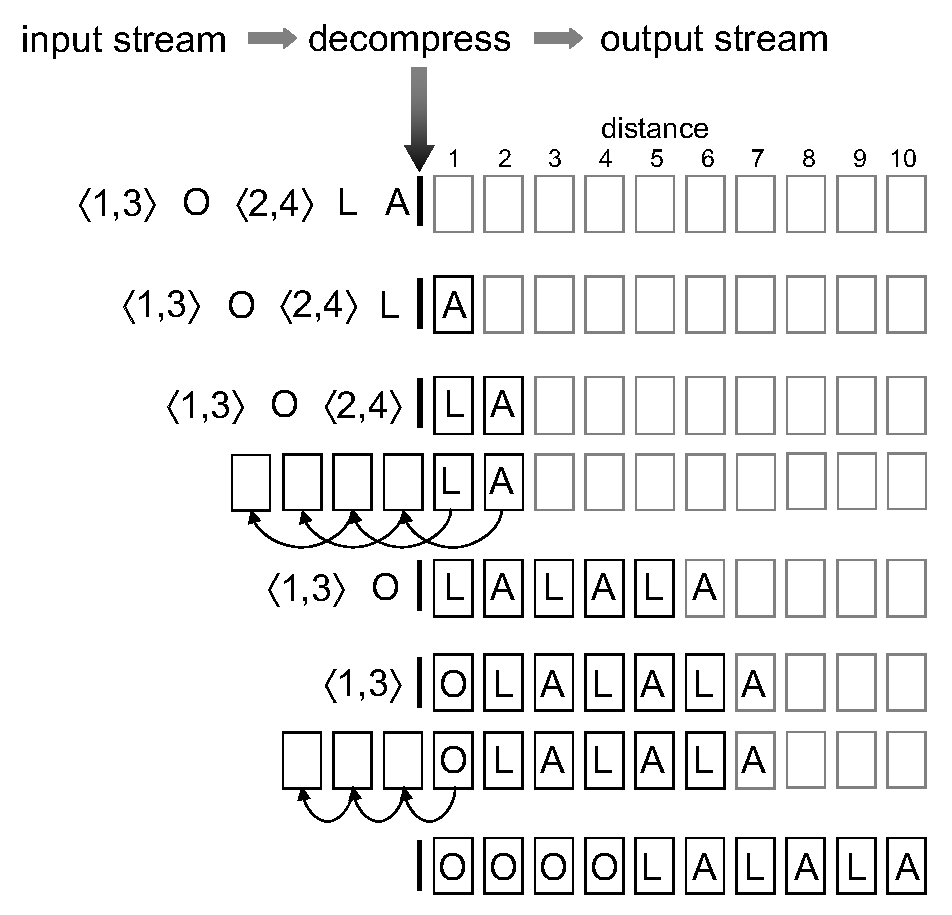
\psfig{file=compression/lz77-figure.eps,width=2.6in}
\caption{Example of LZ77 decompression.
\protect\label{fig:lz77}}
\end{figure}

%% \begin{figure}[t]
%% 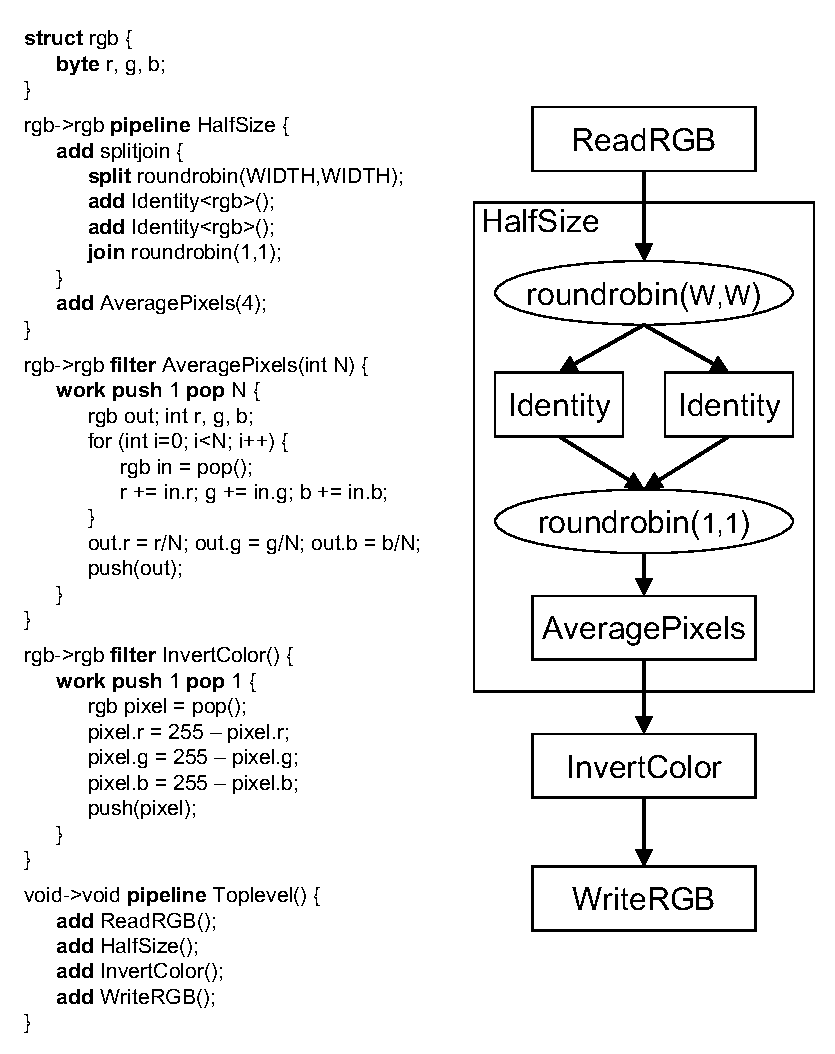
\psfig{file=compression/streamit-figure.eps,width=3.408in}
%% \caption{Example StreamIt program.
%% \protect\label{fig:streamit}}
%% \end{figure}

\section{Mapping into the Compressed Domain}

Our technique allows any cyclo-static dataflow program to operate
directly on LZ77-compressed data.  Rather than modifying the code
within the actors, our transformation treats actors as black boxes and
wraps them in a new execution layer.  The transformation attempts to
preserve as much compression as possible without ever performing an
explicit re-compression step.  While there exist cases in which the
output data will not be as compressed as possible, under certain
conditions the output is guaranteed to be fully compressed (relative
to the compression of the input).  We quantify this issue later.

To describe the mapping into the compressed domain, we consider each
StreamIt construct in turn.  Filters and joiners are described here,
while splitters are described in our technical
report~\cite{techreport}.

\newlength{\oldtextwidth}
\setlength{\oldtextwidth}{7in}
\newcommand{\mynewline}[0]{\\}
\begin{figure*}[t]
{\ninepoint
\begin{minipage}{0.48\oldtextwidth}
{\it Execute a filter in the compressed domain, given that it \\consumes
  $n$ items and produces $m$ items on each execution.}\mynewline
\textsc{Execute-Compressed-Filter}~(int $n$, int $m$) \{\mynewline
\mbox{~~~~}{\bf while true} \{\mynewline
\mbox{~~~~}\mbox{~~~~}{\it /* pass-uncompressed */} \mynewline
\mbox{~~~~}\mbox{~~~~}{\bf if} input {\bf endswith} $n$ values {\bf then}\mynewline
\mbox{~~~~}\mbox{~~~~}\mbox{~~~~}{\bf execute} one call to uncompressed filter\mynewline
\mbox{~~~~}\mbox{~~~~}~\mynewline
\mbox{~~~~}\mbox{~~~~}{\it /* pass-compressed */} \mynewline
\mbox{~~~~}\mbox{~~~~}{\bf else if} input {\bf endswith} $\langle d,c \rangle$\mynewline
\mbox{~~~~}\mbox{~~~~}\mbox{~~~~~~~}{\bf and} $d\%n = 0$ {\bf and} $c \geq n$ {\bf then}\mynewline
\mbox{~~~~}\mbox{~~~~}\mbox{~~~~}{\bf replace} $\langle d,c \rangle$ with $\langle d, c\%n\rangle$ on input\mynewline
\mbox{~~~~}\mbox{~~~~}\mbox{~~~~}{\bf push} $\langle m~d/n, m~(c-c\%n)/n \rangle$ to output\mynewline
\mbox{~~~~}\mbox{~~~~}~\mynewline
\mbox{~~~~}\mbox{~~~~}{\bf else}\mynewline
\mbox{~~~~}\mbox{~~~~}\mbox{~~~~}{\bf let} $\langle d,c \rangle = $ last repeat on input\mynewline
\mbox{~~~~}\mbox{~~~~}\mynewline
\mbox{~~~~}\mbox{~~~~}\mbox{~~~~}{\it /* coarsen-repeat */}\mynewline
\mbox{~~~~}\mbox{~~~~}\mbox{~~~~}{\bf let} $L = \mbox{LCM}(d, n)$\mynewline
\mbox{~~~~}\mbox{~~~~}\mbox{~~~~}{\bf if} $d < L < c$ {\bf then} {\bf replace} $\langle d,c \rangle$\mynewline
\mbox{~~~~}\mbox{~~~~}\mbox{~~~~}\mbox{~~~~}\mbox{~~~~~}with $\langle c - (L - d) \rangle, \langle d, L - d\rangle$ on input\mynewline
\mbox{~~~~}\mbox{~~~~}\mynewline
\mbox{~~~~}\mbox{~~~~}\mbox{~~~~}{\it /* expand */}\mynewline
\mbox{~~~~}\mbox{~~~~}\mbox{~~~~}{\bf else if} $c > 0$ {\bf then}\mynewline
\mbox{~~~~}\mbox{~~~~}\mbox{~~~~}\mbox{~~~~}{\bf decode} $\langle d,c \rangle$ into $\langle d,c-1\rangle,V$ on input\mynewline
\mbox{~~~~}\mbox{~~~~}\mbox{~~~~}{\bf else}\mynewline
\mbox{~~~~}\mbox{~~~~}\mbox{~~~~}\mbox{~~~~}{\bf remove} $\langle d,c \rangle$ from input\mynewline
\mbox{~~~~}\}\mynewline
\}\mynewline
\mbox{~}~~~~~~~~~~~~~~~~~~~~~~~~~~~~~~~~~~~~~~~~~~~{\bf (a)}\mynewline
\end{minipage}
\begin{minipage}{0.52\oldtextwidth}
{\it Execute a roundrobin joiner in the compressed domain, given that
  it inputs $n_1$ items from input1 and $n_2$ items from input2 on
  each execution.}\mynewline
\textsc{Execute-Compressed-Joiner}~(int $n_1$, int $n_2$) \{\mynewline
\mbox{~~~~}{\bf while true} \{\mynewline \mbox{~~~~}\mbox{~~~~}{\it /*
  pass-uncompressed */}\mynewline \mbox{~~~~}\mbox{~~~~}{\bf if}
input1 {\bf endswith} value\mynewline
\mbox{~~~~}\mbox{~~~~}\mbox{~~~~}{\bf transfer} value from input1 to
output\mynewline \mbox{~~~~}\mbox{~~~~}\mynewline
\mbox{~~~~}\mbox{~~~~}{\it /* pass-compressed-long */}\mynewline
\mbox{~~~~}\mbox{~~~~}{\bf else if} input1 {\bf endswith} $\langle
d_1,c_1 \rangle$ {\bf and} $d_1\%n_1 = 0$\mynewline
\mbox{~~~~}\mbox{~~~~}\mbox{~~~~~~~}{\bf and} input2 {\bf endswith}
$\langle d_2,c_2 \rangle$ {\bf and} $d_2\%n_2 = 0$\mynewline
\mbox{~~~~}\mbox{~~~~}\mbox{~~~~~~~}{\bf and} $d_1/n_1 = d_2/n_2$ {\bf
  then}\mynewline \mbox{~~~~}\mbox{~~~~}\mbox{~~~~}{\bf let} $(L_1,
L_2)$ = \textsc{Repeat\_Lengths}($c_1$, $c_2$, {\it pos})\mynewline
\mbox{~~~~}\mbox{~~~~}\mbox{~~~~}{\bf replace} $\langle d_1, c_1
\rangle$ with $\langle d_1, c_1-L_1\rangle$ on input1\mynewline
\mbox{~~~~}\mbox{~~~~}\mbox{~~~~}{\bf replace} $\langle d_1, c_2
\rangle$ with $\langle d_2, c_2-L_2\rangle$ on input2\mynewline
\mbox{~~~~}\mbox{~~~~}\mbox{~~~~}{\bf push} $\langle d_1(n_1+n_2)/n_1,
L_1+L_2 \rangle$ to output\mynewline \mbox{~~~~}\mbox{~~~~}\mynewline
\mbox{~~~~}\mbox{~~~~}{\it /* pass-compressed-short */}\mynewline
\mbox{~~~~}\mbox{~~~~}{\bf else if} input1 {\bf endswith} $\langle
d_1,c_1 \rangle$ {\bf and} $c_1>0$\mynewline
\mbox{~~~~}\mbox{~~~~}\mbox{~~~~}{\bf let} offset = {\bf if} $d\%n_1
\leq \mbox{\it pos}$ {\bf then} {\it pos} {\bf else} $d\%n_1 +
n_2$\mynewline \mbox{~~~~}\mbox{~~~~}\mbox{~~~~}{\bf let} L = {\bf
  min}($c$, \textsc{Join\_Potential}($d$))\mynewline
\mbox{~~~~}\mbox{~~~~}\mbox{~~~~}{\bf replace} $\langle d, c\rangle$
with $\langle d, c - L\rangle$ on input1\mynewline
\mbox{~~~~}\mbox{~~~~}\mbox{~~~~}{\bf push} $\langle
(n_1+n_2)~\mbox{\bf floor}(d/n_1) + \mbox{offset}, L \rangle$ to
output\mynewline \mbox{~~~~}\mbox{~~~~}\mynewline
\mbox{~~~~}\mbox{~~~~}{\it /* prune */}\mynewline
\mbox{~~~~}\mbox{~~~~}{\bf else~} {\it /* input1 endswith}~$\langle
d_1, 0 \rangle$~{\it */}\mynewline
\mbox{~~~~}\mbox{~~~~}\mbox{~~~~}{\bf remove} $\langle d_1,0 \rangle$
from input1\mynewline \mbox{~~~~}\}\mynewline
\}\mynewline
\mbox{~}~~~~~~~~~~~~~~~~~~~~~~~~~~~~~~~~~~~~~~{\bf (b)}\mynewline
\end{minipage}
}
\caption{Translation of (a) filters and (b) joiners into the
  compressed domain.  We use $\%$ to denote a modulo operation.
%Helper functions appear in Figure~\ref{fig:helpers}.
\protect\label{fig:translate}}
\end{figure*}

\subsection{Filters}

The procedure for translating a filter into the compressed domain is
given in Figure~\ref{fig:translate}(a), and an example appears in
Figure~\ref{fig:filter-example}.  The behavior of the
compressed-domain filter can be considered in two pieces.  The first
piece consists of the simple case (annotated {\it pass-uncompressed}
in the code) in which the upcoming inputs to the filter are
uncompressed values.  In this case, the original filter is called with
those inputs, transforming $n$ input items to $m$ output items.  The
rest of the code deals with repeat tokens, attempting to translate
them across the filter with the minimum decompression needed.

The {\bf key idea of the paper} is encapsulated in the {\it
  pass-compressed} case in Figure~\ref{fig:translate}(a).  This rule
specifies how to translate a repeat token directly from a filter's
input tape to a filter's output tape without invoking the filter's
computation.  This translation is possible whenever the repeat
distance $d$ is a multiple of the filter's input rate $n$.  In other
words, the repeat is aligned with the execution boundaries of the
actor, so invoking the actor would produce the same results as before.
In transferring the repeat token to the output tape, two adjustments
are made: 1) the distance and count are scaled by a factor of $m/n$ to
reflect possible differences between the output ($m$) and input ($n$)
rates of the actor, and 2) if the count is not an even multiple of the
input rate, then some leftover items ($c\%n$, where $\%$ represents
the modulo operation) are left on the input tape.

In cases where the repeat distance does not match the granularity of
the actor, the distance can sometimes be adjusted to allow
compressed-domain processing.  The {\it coarsen-repeat} rule
represents such an adjustment.  Consider that a filter inputs two
items at a time, but encounters a long repeat with distance three and
count 100.  That is, the input stream contains a regular pattern of
values with periodicity three.  Though consecutive executions of the
filter are aligned at different offsets in this pattern, every third
filter execution (spanning six values) falls at the same alignment.
In general, a repeat with distance $d$ can be exploited by a filter
with input rate $n$ by expanding the distance to $\mbox{LCM}(d, n)$.
In order to perform this expansion, the count must be greater than the
distance, as otherwise the repeat references old data that may have no
periodicity.  Also, the stream needs to be padded with $\mbox{LCM}-d$
values before the coarsened repeat can begin; this padding takes the
form of a shorter repeat using the original distance.

A second way to adjust a repeat token for compressed-domain processing
is by changing its count rather than its distance (rule {\it expand}).
The expand rule is invoked if a repeat has a count less than $n$, if
it is unaligned with the boundaries of an actor's execution, or if its
distance is not a multiple of $n$ (and cannot be coarsened
appropriately).  The expand rule decodes a single value from a repeat
token, thereby decreasing its count by one; the rest of the repeat may
become aligned later.  If the count of a repeat reaches zero, it is
eliminated.

Note that the {\it expand} rule requires partial decompression of the
data stream.  In order to perform this decompression, it may be
necessary to maintain an auxiliary data structure--separate from the
filter's input stream--that holds a complete window of decompressed
data.  This auxiliary structure is needed because the sliding-window
dictionary of LZ77 makes it difficult to decode one element without
decoding others.  However, even if the stream is fully decompressed in
parallel with the main computation, our technique retains many
benefits because the filters still operate on the compressed stream;
the volume of data processed is reduced, and the cost of
re-compression is averted.  For general algorithms such as gzip,
compression can be up to 10x slower than
decompression~\cite{ziviani00compression}.

%% The alignment stage sometimes needs to partially decompress the
%% data in the stream.  Due to the sliding-window dictionary in LZ77,
%% in general it is difficult to decode only a few items without
%% decompressing others.  Thus, our formulation assumes that a fully
%% decompressed version of the stream is available; the transition
%% rules access the decompressed data using the \mbox{\it decode}
%% function, which returns the sequence of values represented by a
%% repeat token at its current position in the stream.  However, in
%% practice, this decompression can be avoided whenever the repeat
%% distance is the same as the window size, as this simply causes a
%% value in the window to be overwritten by itself.  This case is very
%% common in several practical compression formats; for example, in
%% Apple Animation, the vast majority of repeats reference the same
%% pixel in the previous frame (which is also the window size), and
%% thus most decompression is avoided.  In run-length encoding, the
%% repeat distance and the window size are always equal to one, so no
%% decompression is needed.  While general LZ77 does require a
%% decompressed window to be maintained, our technique still offers
%% significant benefits by computing on a smaller volume of data and
%% avoiding the cost of re-compression.  For general algorithms such
%% as gzip, compression can be up to 10x slower than
%% decompression~\cite{ziviani00compression}.

\begin{figure*}[t]
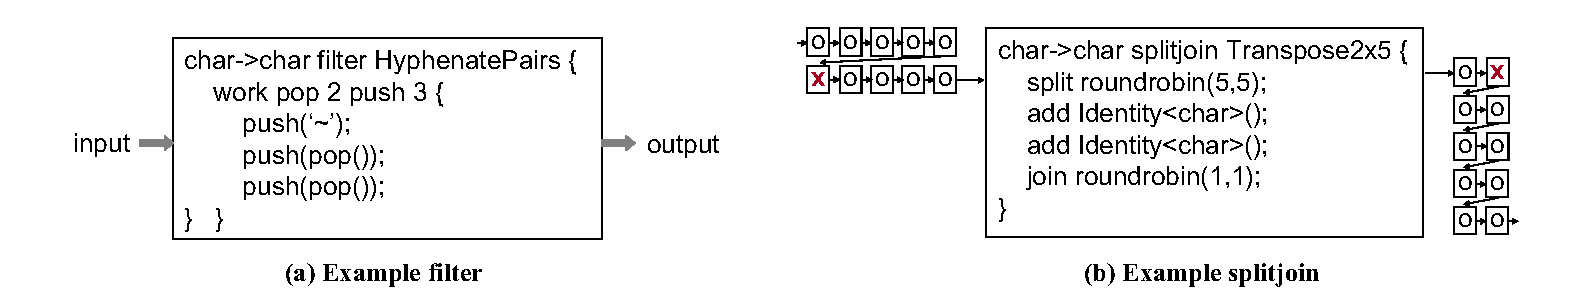
\psfig{file=compression/compressed-filters-in-streamit.eps,width=\textwidth}
\caption{Example filter, splitter, and joiner in StreamIt.  The
  splitter and joiner combine to form a Transpose. Translation to the
  compressed domain is illustrated in Figures~\ref{fig:filter-example}
  and~\ref{fig:sj-example}.\protect\label{fig:streamit-example}}
\end{figure*}

\begin{figure*}[t]
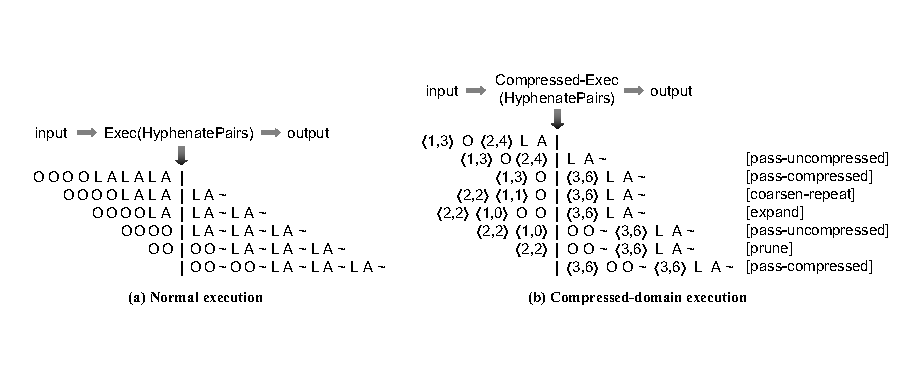
\psfig{file=compression/compressed-filter-example.eps,width=\textwidth}
\caption{Example execution of a filter in the uncompressed and
  compressed domains.  See Figure~\ref{fig:streamit-example}(a) for the
  source filter.\protect\label{fig:filter-example}}
\end{figure*}

\subsection{Joiners}

%% It is necessary to consider splitters and joiners separately from
%% general-purpose actors because of their pass-through semantics: the
%% inputs are distributed to the outputs without performing any
%% computation.  Our translation to the compressed domain leverages this
%% fact to preserve considerably more compression than would be possible
%% if splitters and joiners were viewed as opaque computational nodes
%% with multiple inputs and multiple outputs.

The procedure for executing a joiner in the compressed domain appears
in Figure~\ref{fig:translate}(b), while an example appears in
Figure~\ref{fig:sj-example}.  To simplify the presentation, we
consider a joiner with only two input streams.  This captures all of
the fundamental ideas; extension to additional streams is
straightforward.  In addition, we use the following notations:

\begin{figure*}[t]
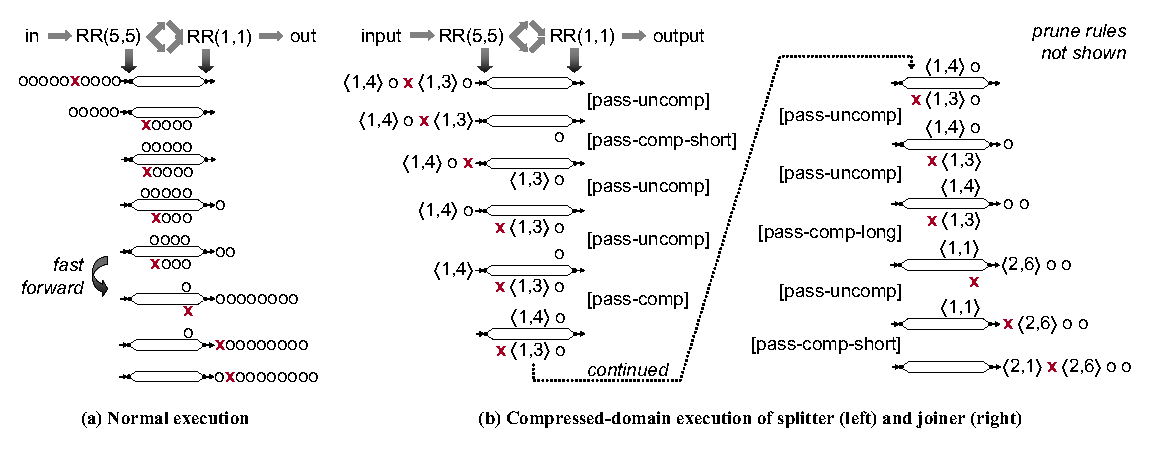
\psfig{file=compression/compressed-splitjoin-example.eps,width=\textwidth}
\caption{Example execution of splitters and joiners in the compressed
  domain.  As illustrated by the input/output pairs in
  Figure~\ref{fig:streamit-example}(b), the example performs a transpose
  of a 2x5 matrix.  When the matrix is linearized as shown here, the
  input stream traverses the elements row-wise while the output stream
  traverses column-wise.  Due to redundancy in the matrix, this
  reordering can be done largely in the compressed domain.
  \protect\label{fig:sj-example}}
\end{figure*}

\begin{itemize}

\item As mentioned previously, splitters and joiners adopt a
  fine-grained cyclo-static execution model, in which each execution
  step transfers only one item from an input tape to an output tape.
  That is, a roundrobin$(n_1, n_2)$ joiner has $n_1 + n_2$ distinct
  execution steps.  We refer to every group of $n_1 + n_2$ steps as an
  {\it execution cycle}.

\item The pseudocode in Figure~\ref{fig:translate} assumes, without
  loss of generality, that the next execution step of the joiner will
  read from the first input stream (input1).

\item We use $\pos$ to denote the number of items (in terms of the
  uncompressed domain) that have already been read from the current
  input stream (input1) in the current execution cycle.  For brevity,
  the pseudocode does not maintain the value of $\pos$, though it is
  straightforward to do so.

\end{itemize}

\begin{figure}[t]
{\elevenpoint
\begin{minipage}{0.1in}
\vspace{-1.75pt}
{\it // // // // // //}
\end{minipage}
\begin{minipage}{3.23in}
{\it Given that $c_1$ and $c_2$ compressed items are available on the
  first and second input streams of a joiner, returns the number of
  items that can be read from each input before one of them is
  exhausted.  Assumes that the joiner is currently reading from the
  first input stream, from which \mbox{pos} items have previously been
  consumed in the current execution cycle.}
\end{minipage}
\textsc{Repeat\_Lengths}$(c_1, c_2, \pos )$~returns~(int,~int)~\{\\
\tab{\it // the number of complete joiner cycles, and the leftovers}\\
\tab$\mbox{total\_cycles} = \mbox{floor}(c/(n_1 + n_2))$\\
\tab$\mbox{leftover}_1 = c_1 - \mbox{total\_cycles} * n_1$\\
\tab$\mbox{leftover}_2 = c_2 - \mbox{total\_cycles} * n_2$\\
~ \vspace{-6pt}\\
\tab{\it // the last partial cycle may end in three regions:}\\
\tab$\mbox{\bf if~} \mbox{leftover}_1 \leq n_1 - \pos$~\{\\
\tab\tab{\it // 1. in reading from the first input stream}\\
\tab\tab$L_1 = \mbox{leftover}_1$\\
\tab\tab$L_2 = 0$\\
\tab$\} \mbox{\bf~else if~} \mbox{leftover}_2 \leq n_2~\{$\\
\tab\tab{\it // 2. in subsequent reading from the second input stream}\\
\tab\tab$L_1 = n_1-\pos$\\
\tab\tab$L_2 = \mbox{leftover}_2$\\
\tab\} \mbox{\bf ~else} \{\\
\tab\tab{\it // 3. in wrap-around reading from the first input stream}\\
\tab\tab$L_1 = \mbox{leftover}_1$\\
\tab\tab$L_2 = n_2$\\
\tab\}\\
~ \vspace{-6pt}\\ 
\tab$\mbox{\bf return~}(n_1*\mbox{total\_cycles} + L_1, n_2*\mbox{total\_cycles} + L_2)$
\}}
\caption{The \textsc{Repeat\_Lengths} function is called during
  compressed joiner execution.  In the case where the input tokens to
  the joiner have compatible repeat distances, it calculates the
  maximum repeat lengths that can be passed to the
  output.\protect\label{fig:repeat-lengths}}
\end{figure}

There are two ways to pass repeat tokens through a joiner.  If the
input streams contain compatible repeat tokens, then they can be
combined into a long repeat that spans multiple execution cycles;
otherwise, a shorter repeat is extracted from only one of the streams.

The first and most powerful way to execute joiners in the compressed
domain is to combine repeat tokens from both input streams (case {\it
  pass-compressed-long} in Figure~\ref{fig:translate}b).  For this to
be possible, both repeat distances must be the same multiple of their
respective joiner weight ($n_1$ or $n_2$); the combined token has a
repeat distance that is a multiple of $n_1 + n_2$.  The
\textsc{Repeat\_Lengths} routine (detailed in
Figure~\ref{fig:repeat-lengths}) calculates the maximum repeat length
depending on the current position of the joiner and the repeat lengths
of the inputs.

The second mode of compressed joiner execution ({\it
  pass-compressed-short}) inputs only a single repeat token,
extracting the maximum length that can safely move to the output.  The
\textsc{Join\_Potential} routine (detailed in
Figure~\ref{fig:join-potential}) determines how much of the repeat can
be moved to the output before the data referenced would have
originated from a different input stream.

\section{Supported File Formats}
\label{sec:formats}

As LZ77 refers to a compression algorithm rather than a complete
compression format, there are additional factors to consider in
mapping computations to real-world image and video codecs.  Some
codecs are a subset of LZ77, utilizing only run-length encoding or a
fixed window size; these are supported very efficiently by our
technique.  Others are a superset of LZ77, incorporating additional
techniques such as delta coding or Huffman coding; these may incur
additional processing overhead.  In the following sections, we
describe the practical considerations involved in targeting various
compression formats with our technique.  Formats are ordered by
approximate goodness of the achievable mapping.

\subsection{High-Efficiency Mappings}
\label{sec:formats-good}

All of the formats in this category can be considered to be subsets of
LZ77.

\paragraph{Apple Animation.}  
The Apple Animation codec (which forms the basis for our experimental
evaluation) is supported as part of the Quicktime MOV container
format.  It serves as an industry standard for exchanging computer
animations and digital video content before they are rendered to lossy
formats for final distribution~\cite[p.~106]{adobe-anim}\cite[p.~284]{harrington-anim} \cite[p.~367]{long-anim}\cite[p.~280]{pogue-anim}.

The Animation codec represents a restricted form of LZ77 in which
repeat distances are limited to two values: a full frame or a single
pixel.  A repeat across frames indicates that a stretch of pixels did
not change from one frame to the next, while a repeat across pixels
indicates that a stretch of pixels has the same color within a frame.
% mention bit depths?

\paragraph{Flic Video.}
Flic Video files (FLI/FLC) were originally produced by Autodesk
Animator and are still supported by many animation packages today.
Their compression of frame data is almost identical to Apple
Animation.

\begin{figure}[t]
\begin{minipage}{0.1in}
\vspace{-1.75pt}
{\it // // // // //}
\end{minipage}
\begin{minipage}{3.23in}
{\it Given a repeat token with distance $d$ on the current input
  stream of a joiner, returns the maximum count of a repeat token that
  could safely be emitted to the output stream.  Assumes that only a
  single repeat token is available (i.e., the {\tt
    pass-compressed-long} rule does not apply).}
\end{minipage}
\textsc{Join\_Potential}$(d)$~returns~int~\{\\
\tab$\mbox{offset} = d$\%$n_1$\\
\tab$\mbox{{\bf if~}} \mbox{offset} \leq \pos ~\{$\\
\tab\tab{\it // repeat for remainder of this execution cycle}\\
\tab\tab$\mbox{\bf return~} n_1 - \pos$\\
\tab$\} \mbox{\bf ~else} ~\{$\\
\tab\tab{\it // repeat until referenced data goes out of range}\\
\tab\tab$\mbox{\bf return~} \mbox{offset} - \pos$\\
\tab$\}$\\
\}
\caption{The \textsc{Join\_Potential} function is called during
  compressed joiner execution.  In the case where the input tokens to
  the joiner have incompatible repeat distances, it calculates the
  maximum length of the current token that may be passable to the
  output. \protect\label{fig:join-potential}}
\end{figure}

\paragraph{Microsoft RLE.}
Microsoft RLE compression can appear in both BMP images and AVI
animations.  Apart from bit-depth and formatting details, its
capabilities are identical to Apple Animation; it can perform
run-length encoding within a frame, and can skip over pixels to
exploit inter-frame redundancy.

\paragraph{Targa.}
The Truevision Targa (TGA) format is a simple image format that is
widely used to render frame sequences in the computer animation and
video industries.  The format includes an optional RLE compression
stage, making it a good target for our technique.

\paragraph{PXY.}
The pxy format is a research-based image format designed to support
efficient transpose and rotation of black-and-white
images~\cite{shoji95}.  It consists of the series of $(x,y)$
coordinates at which the image changes color during a horizontal scan.
As this information can be converted to a run-length encoding, it can
also be targetted by our technique.

\subsection{Medium-Efficiency Mappings}
\label{sec:formats-med}

While the formats in this category utilize an encoding that is
compatible with LZ77, they incur extra overhead because the data is
reorganized prior to the compression stage.

\paragraph{Planar RGB.}
The Planar RGB video format is supported by Apple Quicktime files.  It
utilizes run-length encoding for pixels within a frame, with partial
support for expressing inter-frame repeats (only the end of lines can
be skipped).  The red, green, and blue planes are encoded separately
in order to increase compression.  For user transformations that need
to process red, green, and blue values together, this introduces
additional alignment overhead when applying our technique.

\paragraph{OpenEXR.}
OpenEXR is an emerging image format (backed by Industrial Light and
Magic) for use in digital film.  It offers several compression
options, including run-length encoding, zip, and wavelet-based
compression.  However, in run-length encoding mode, the low and high
bytes of the pixels are separated and encoded as separate run-length
sequences; this enables pixels with variations in the low bytes to
nonetheless benefit from compression of the high bytes.  As most user
transformations would utilize the entire bit-width of the pixel, our
technique suffers additional alignment overhead in processing these
files.

\subsection{Low-Efficiency Mappings}
\label{sec:formats-bad}

The formats in this category are supersets of LZ77.  While our
technique could offer some gains in exploiting the LZ77 compression,
it would have to undo any compression sitting on top of LZ77 and
offers limited benefit for filters (as in PNG) applied underneath
LZ77.

\paragraph{DEFLATE.}
DEFLATE is a general-purpose algorithm that provides all of the
compression for popular formats such as ZIP and GZIP.  The algorithm
consists of a full LZ77 encoder followed by Huffman coding, which
resizes the symbols in the stream to match their usage frequencies.
In targeting ZIP or GZIP with our transformations, we would first
have to undo the Huffman coding (unless the application simply
reordered data, in which case the coding could remain intact).  Though
Huffman decoding is a lightweight lookup operation, it would also
increase the memory footprint.  In addition, as DEFLATE's LZ77
algorithm operates on individual bytes, there may be an exaggerated
alignment cost if the application operates on a larger word size.

\paragraph{TSCC.}
The TechSmith Screen Capture Codec is very similar to Microsoft RLE,
except that the final output is further compressed using DEFLATE.
Thus, any overheads incurred by our technique on DEFLATE also extend
to TSCC.

\paragraph{PNG.}
The PNG image format also relies on DEFLATE to compress the pixels in
the image.  However, before running DEFLATE, the pixels are usually
filtered with a delta encoding; each pixel is replaced with the
difference between its value and a predicted value, where the
prediction is a linear combination of neighboring pixels.  While
program segments that compute a linear function~\cite{aalamb} could
perhaps be mapped to this compressed format, our current technique
only applies if the delta encoding is turned off.  Even in this
scenario, there is a large amount of overhead due to the Huffman
coding in DEFLATE.

\begin{table*}[t]
\hspace{-0.26in}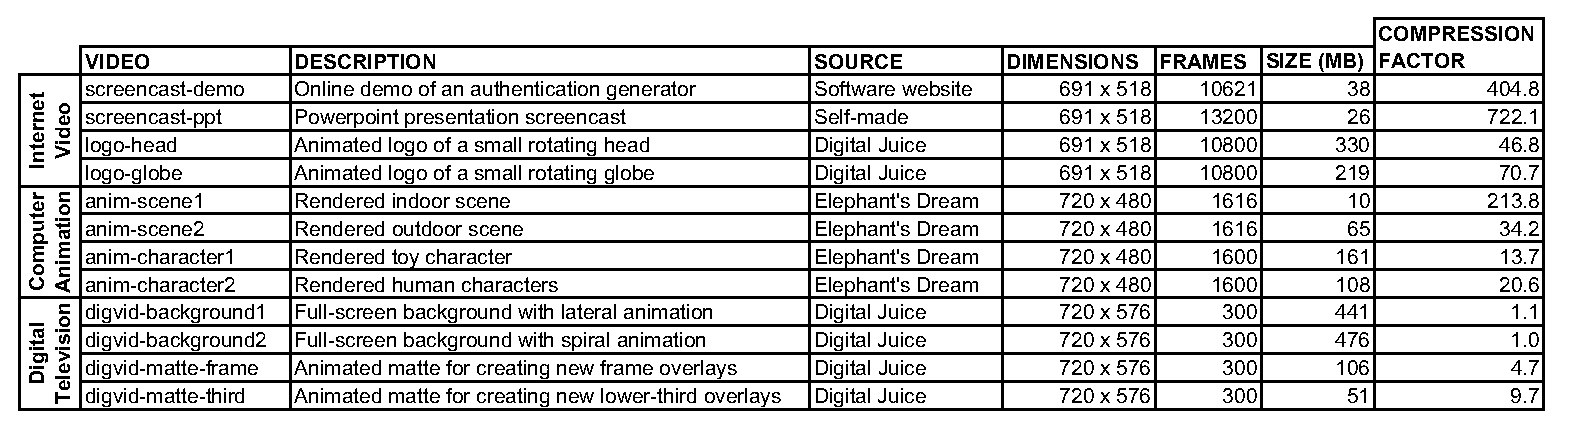
\psfig{file=compression/table-benchmarks.eps,width=7.02in}
\caption{Characteristics of the video workloads.
\protect\label{tab:videos}}
\end{table*}

\section{Experimental Evaluation}

To demonstrate the potential benefits of mapping into the compressed
domain, we implemented a few of our transformations as part of the
StreamIt compiler.  Our current implementation supports two
computational patterns: 1) transforming each individual element of a
stream (via a pop-1, push-1 filter), and 2) combining the elements of
two streams (via a roundrobin(1,1) joiner and a pop-2, push-1 filter).
The program can contain any number of filters that perform arbitrary
computations, so long as the I/O rates match these patterns.  While we
look forward to performing a broader implementation in future work,
these two building blocks are sufficient to express a number of useful
programs and to characterize the performance of the technique.

Our evaluation focuses on applications in digital video editing.
Given StreamIt source code that operates on pixels from each frame of
a video, the StreamIt compiler maps the computation into the
compressed domain and emits executable plugins for two popular video
editing tools, MEncoder and Blender.  The plugins are written for the
Apple Animation format (see Section~\ref{sec:formats-good}).

Our benchmarks fall into two categories: 1) pixel transformations,
such as brightness, contrast, and color inversion, which adjust pixels
within a single video, and 2) video compositing, in which one video is
combined with another as an overlay or mask.

The main results of our evaluation are:
\begin{itemize}

\item Operating directly on compressed data offers a speedup roughly
proportional to the compression factor in the resulting video.

\item For pixel transformations, speedups range from 2.5x to 471x,
  with a median of 17x.  Output sizes are within 0.1\% of input sizes
  and about 5\% larger (median) than a full re-compression.

\item For video compositing, speedups range from 1.1x to 32x, with a
  median of 6.6x.  Output files retain a sizable compression ratio
  (1.0x to 44x) and are about 52\% larger (median) than a full
  re-compression.

\end{itemize}
The following sections provide more details on our video workloads,
the evaluation of pixel transformations, and the evaluation of video
compositing.

\subsection{Video Workloads}

Our evaluation utilizes a suite of 12 video workloads that are
described in Table~\ref{tab:videos}; some of the videos are also
pictured in Figure~\ref{fig:videos}.  The suite represents three
common usage scenarios for lossless video formats: Internet
screencasts, computer animation, and digital television production.
While videos in each area are often rendered to a lossy format for
final distribution, lossless codecs are preferred during the editing
process to avoid accumulating compression artifacts.  All of our
source videos are in the Apple Animation format (described in
Section~\ref{sec:formats-good}), which is widely used by video editing
professionals~\cite[p.~106]{adobe-anim} \cite[p.~284]{harrington-anim}
\cite[p.~367]{long-anim} \cite[p.~280]{pogue-anim}.  The Apple
Animation format is also popular for capturing video from the screen
or camera, as the encoder is relatively fast.

Our suite of videos is assembled from a variety of realistic and
industry-standard sources.  The first screencast is an online demo of
an authentication generator for rails~\cite{auth-demo}; the second is
a PowerPoint presentation (including animations), captured using
Camtasia Studio.  As Internet content is often watermarked with a logo
or advertisement, we include two animated logos in the ``Internet
video'' category.  These logos are taken from Digital
Juice~\cite{digital-juice}, a standard source for professional
animations, and rendered to Apple Animation format using their
software.  The animated logos are rendered full-frame (with the logo
in the corner) because compositing operations in our testbed (Blender)
are done on equal-sized videos.

The computer animation clips are derived from Elephant's Dream, a
short film with entirely open-source content~\cite{elephants-dream};
our videos are rendered from source using Blender.  Finally, the
digital television content is also taken from a Digital Juice
library~\cite{digital-juice}.  The backgrounds represent
high-resolution, rotating backdrops as might appear in the
introduction to a program.  The mattes are black-and-white animations
that can be used to synthesize a smaller overlay (such as a frame or a
``lower third'', often used for text) from a full animated background
(see Figure~\ref{fig:videos}b for an example).

The videos exhibit a wide range of compression factors.  The
screencasts have very high compression ($\sim$400x-700x) because only
a small part of the screen (e.g., a mouse, menu, or PowerPoint bullet)
is changing on any given frame; the Apple Animation format compresses
the inter-frame redundancy.  The compression for {\tt anim-scene1} is
also in excess of 200x because motion is limited to a small animated
character.  The animated logos are the next most compressed
($\sim$50-70x), influenced largely by the constant blank region
outside the logo.  The computer animation content ($\sim$10-30x
compression) has a high level of detail but benefits from both
inter-frame and intra-frame redundancy, as some rendered regions have
constant color.  Next are the digital video mattes ($\sim$5-10x
compression), which have fine-grained motion in some sections.
Finally, the digital video backgrounds offer almost no compression
gains (1.0-1.1x) under Apple Animation, as they have pervasive motion
and detail across the entire frame.

The Apple Animation format supports various bit depths.  All of our
source videos use 32 bits per pixel, allocating a single byte for each
of the red, green, blue, and alpha channels.

\subsection{Pixel Transformations}

The pixel transformations adjust the color of each pixel in a uniform
way.  We evaluated three transformations:
\begin{itemize}
\item Brightness adjustment, which increases each RGB value by a value
of 20 (saturating at 255).
\item Contrast adjustment, which moves each RGB value away from the
center (128) by a factor of 1.2 (saturating at 0 and 255).

\item Color inversion, which subtracts each RGB value from 255 (useful
  for improving the readability of screencasts or for reversing the
  effect of video mattes).

\end{itemize}

We implemented each transformation as a single StreamIt filter that
transforms one pixel to another.  Because the filter has a pop rate of
one, it does not incur any alignment overhead.

\subsubsection{Setup}

The pixel transformations were compiled into plugins for MEncoder, a
popular command-line tool (bundled with MPlayer) for video decoding,
encoding, and filtering.  MEncoder relies on the FFMPEG library to
decode the Apple Animation format; as FFMPEG lacked an encoder for
this format, the authors implemented one.  Additionally, as MEncoder
lacks an interface for toggling only brightness or contrast, the
baseline configuration was implemented by the authors.

The baseline configuration performs decompression, pixel
transformations, then re-compression.  Because the main video frame is
updated incrementally by the decoder, the pixel transformations are
unable to modify the frame in place (otherwise pixels present across
frames would be transformed multiple times).  Thus, the baseline
transformation writes to a separate location in memory.  The optimized
configuration performs pixel transformations directly on the
compressed data, avoiding data expansion implied by decompression and
multiple frame buffers, before copying the data to the output file.

\begin{table*}[t]
\hspace{-0.26in}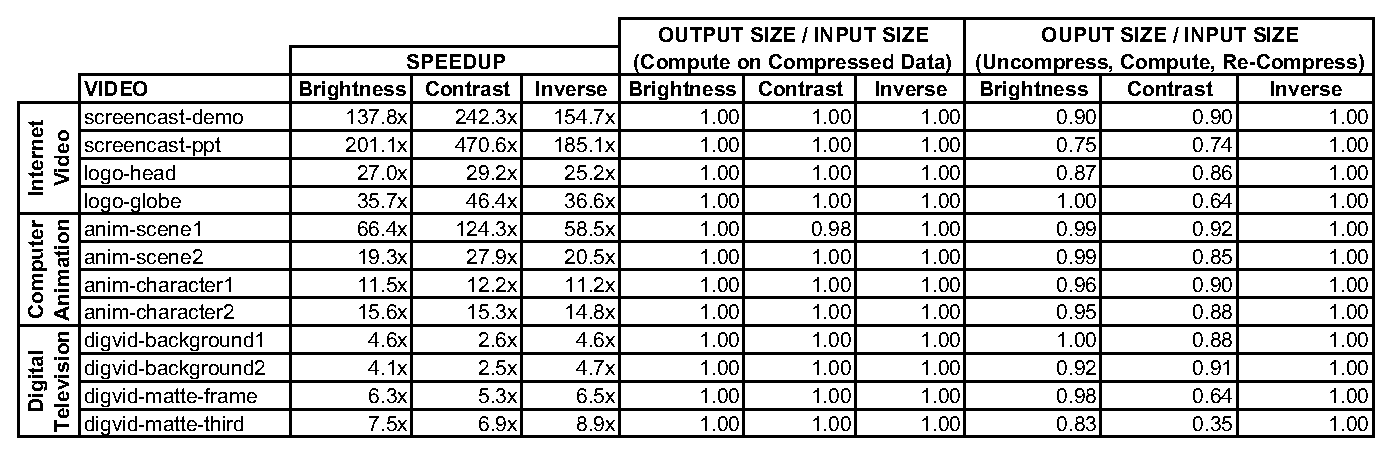
\psfig{file=compression/table-pixel-speedup.eps,width=7.02in}
\caption{Results for pixel transformations.
\protect\label{tab:pixel-speedup}}
\end{table*}

Our evaluation platform is a dual-processor Intel Xeon (2.2 GHz) with
2 GB of RAM.  As all of our applications are single-threaded, the
second processor is not utilized.  For the timing measurements, we
execute each program five times and report the median user time.

\subsubsection{Results}

Detailed results for the pixel transformations appear in
Table~\ref{tab:pixel-speedup}.  Figure~\ref{fig:pixel-speedup}
illustrates the speedups, which range from 2.5x to 471x.  As
illustrated in Figure~\ref{fig:speedup-scatter}, the speedups are
closely correlated with the compression factor in the original video.
For the highly-compressed screencasts and {\tt anim-scene1}, speedups
range from 58x to 471x.  For the medium-compression computer
animations (including the animated logos), speedups range from 11x to
46x.  And for the low-compression digital television content, speedups
range from 2.5x to 8.9x.

There are two distinct reasons for the speedups observed.  First, by
avoiding the decompression stage, computing on compressed data reduces
the volume of data that needs to be stored, manipulated, and
transformed.  This savings is directly related to the compression
factor and is responsible for the upwards slope of the graph in
Figure~\ref{fig:speedup-scatter}.  Second, computing on compressed
data eliminates the algorithmic complexity of re-compression.  For the
Apple Animation format, the cost of compressing a given frame does not
increase with the compression factor (if anything, it decreases as
fewer pixels need a fine-grained encoding).  Thus, the baseline
devotes roughly constant runtime to re-compressing each video, which
explains the positive intercept in the graph of
Figure~\ref{fig:speedup-scatter}.

The impact of re-compression is especially evident in the digital
television examples.  Despite a compression factor of 1.0 on {\tt
digvid-background2}, our technique offers a 4.7x speedup on color
inversion.  Application profiling confirms that 
% NOTE: I profiled the hand-coded version rather than the StreamIt
% version.  It had a speedup of 5.5x rather than 4.7x
73\% of the baseline runtime is spent in the encoder; as this stage is
absent from the optimized version, it accounts for $1/(1-0.73) = 3.7$x
of the speedup.  The remaining speedup in this case is due to the
extra frame buffer (and associated memory operations) in the
decompression stage of the baseline configuration.
%
%(Don't really understand these profiling numbers yet)
%
%Note that videos with larger compression ratios spend
%a smaller fraction of time in the encoder; for example, color
%inversion on {\tt screencast1-demo} spends only 5\% of its time in the
%encoder (and 65\% of the time doing the transformation itself).

Another important aspect of the results is the size of the output
files produced.  Apart from the first frame of a video\footnote{In the
Apple Animation format, the first frame is encoded as if the previous
frame was black.  Thus, adjusting the color of black pixels in the
first frame may increase the size of the file, as it removes
inter-frame redundancy.}, performing pixel transformations directly on
compressed data will never increase the size of the file.  This is
illustrated in the middle columns of Table~\ref{tab:pixel-speedup}, in
which the output sizes are mostly equal to the input sizes (up to 2
decimal places).  The only exception is contrast adjustment on {\tt
anim-scene1}, in which the output is 2\% smaller than the input due to
variations in the first frame; for the same reason, some cases
experience a 0.1\% increase in size (not visisble in the table).

\begin{figure}[t]
\centering
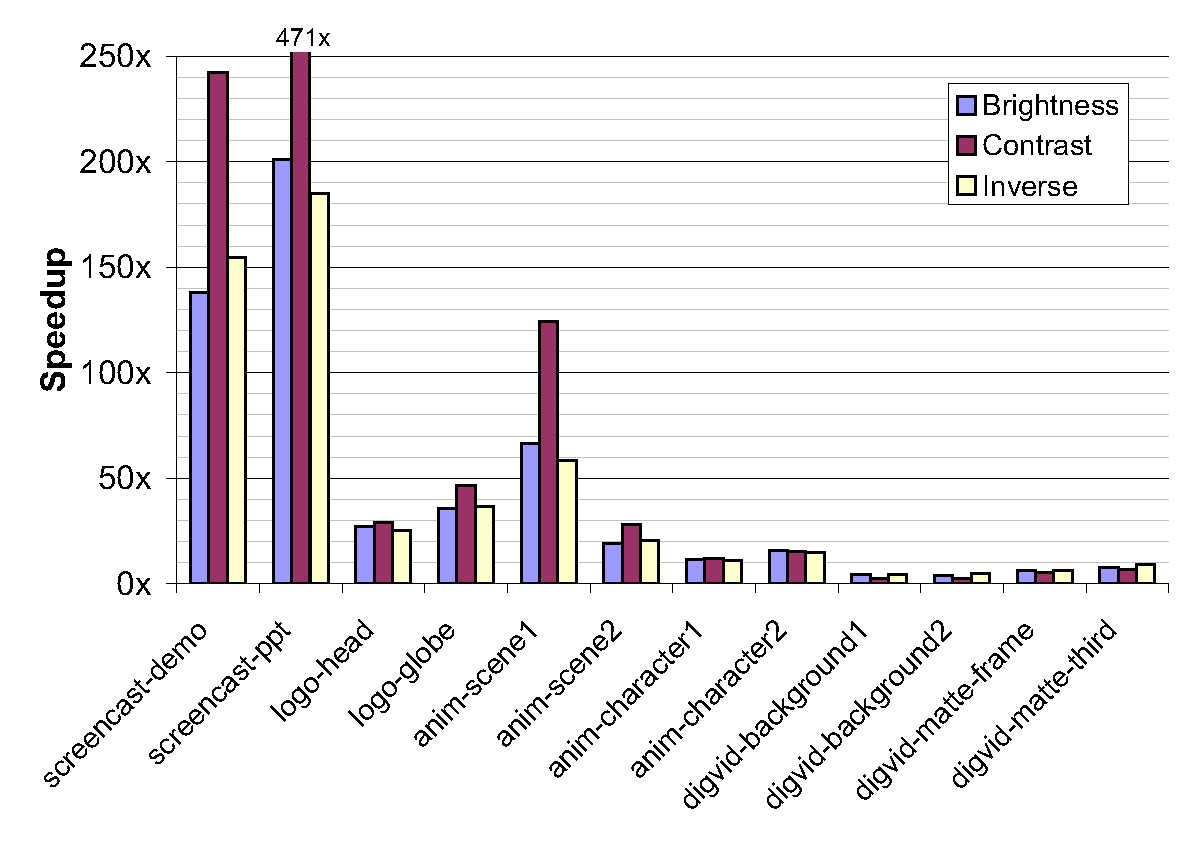
\psfig{file=compression/graph-speedup-pixel.eps,width=4.355in}
\caption{Speedup on pixel transformations.
\protect\label{fig:pixel-speedup}}
\end{figure}

Though computing on compressed data has virtually no effect on the
file size, there are some cases in which the pixel transformation
increases the redundancy in the video and an additional re-compression
step could compress the output even further than the original input.
This potential benefit is illustrated in the last three columns of
Table~\ref{tab:pixel-speedup}, which track the output size of the
baseline configuration (including a re-compression stage) versus the
original input.  For the inverse transformation, no additional
compression is possible because inverse is a 1-to-1 transform: two
pixels have equal values in the output file if and only if they have
equal values in the input file.  However, the brightness and contrast
transformations may map distinct input values to the same output
value, due to the saturating arithmetic.  In such cases, the
re-compression stage can shrink the file to as low as 0.75x
(brightness) and 0.35x (contrast) its original size.  These are
extreme cases in which many pixels are close to the saturating point;
the median re-compression (across brightness and contrast) is only
10\%.

To achieve the minimal file size whenever possible, future work will
explore integrating a lightweight re-compression stage into the
compressed processing technique.  Because most of the compression is
already in place, it should be possible to improve the compression
ratio without running the full encoder (e.g., run-length encoded
regions can be extended without being rediscovered).  

% (The following comment didn't make sense -- to do the full
% re-compression, you would need to start from a decompressed stream,
% which has the full data volume.)
%
% Even running the full encoding algorithm (in place on the compressed
% data) may leave us with significant speedups, as much of the
% improvement comes from decreased data volume rather than decreased
% re-compression cost.

\subsection{Video Compositing}

In video compositing, two videos are combined using a specific
function to derive each output pixel from a pair of input pixels (see
Figure~\ref{fig:videos}).  In the case of subtitling, animated logos,
and computer graphics, an alpha-under transformation is common; it
overlays one video on top of another using the transparency
information in the alpha channel.  In applying an animated matte, the
videos are combined with a multiply operation, thereby masking the
output according to the brightness of the matte.  For our experiments,
we generated composites using each foreground/background pair within a
given application area, yielding a total of 12 composites.

In StreamIt, we implemented each compositing operation as a
roundrobin(1,1) joiner (to interleave the streams) followed by a
filter (to combine the pixel values).  The intuition of the
compressed-domain execution is that if both streams have the same kind
of repeat (inter-frame or intra-frame), then the repeat is copied
directly to the output.  If they have different kinds of repeats, or
if one stream is uncompressed, then both streams are uncompressed.

\subsubsection{Setup}

The compositing operations were compiled into plugins for Blender, a
popular tool for modeling, rendering, and post-processing 3-D
animations.  Blender has logged 1.8 million downloads in the last
year~\cite{blender-stats} and was used in the production of Spiderman
2~\cite{blender-wikipedia}.  Like MEncoder, Blender relies on the
FFMPEG library for video coding, so we utilize the same Apple
Animation decoder/encoder as in the pixel transformations.

As Blender already includes support for video compositing, we use its
implementation as our baseline.  The compositing operations have
already been hand-tuned for performance; the implementation of
alpha-under includes multiple shortcuts, unrolled loops, and the
following comment: ``this complex optimalisation is because the
'skybuf' can be crossed in''.  We further improved the baseline
performance by patching other parts of the Blender source base, which
were designed around 3-D rendering and are more general than needed
for video editing.  We removed two redundant vertical flips for each
frame, two redundant BGRA-RGBA conversions, and redundant memory
allocation/deallocation for each frame.
% did not mention removal of O(frames^2) linked list search, although 
% this fell out of removing the redundant memory deallocation

\begin{figure}[t]
\centering
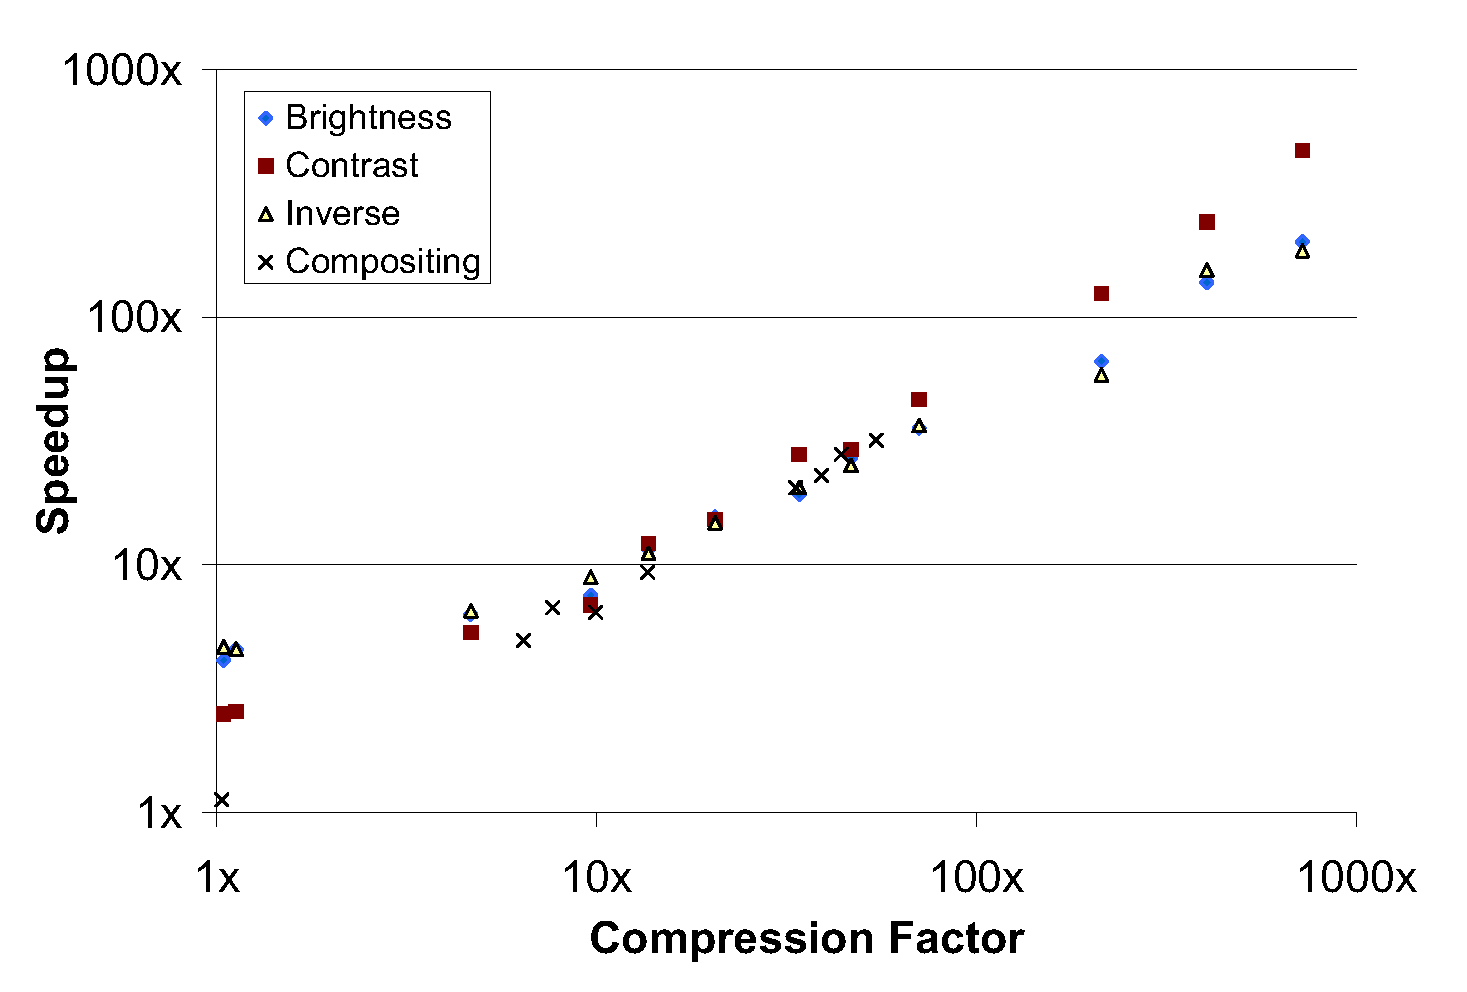
\psfig{file=compression/graph-speedup-scatter.eps,width=4.511in}
\caption{Speedup vs. compression factor for all transformations.
\protect\label{fig:speedup-scatter}}
\end{figure}

\begin{figure}[t]
\centering
\begin{minipage}{0.3\textwidth}
\centering
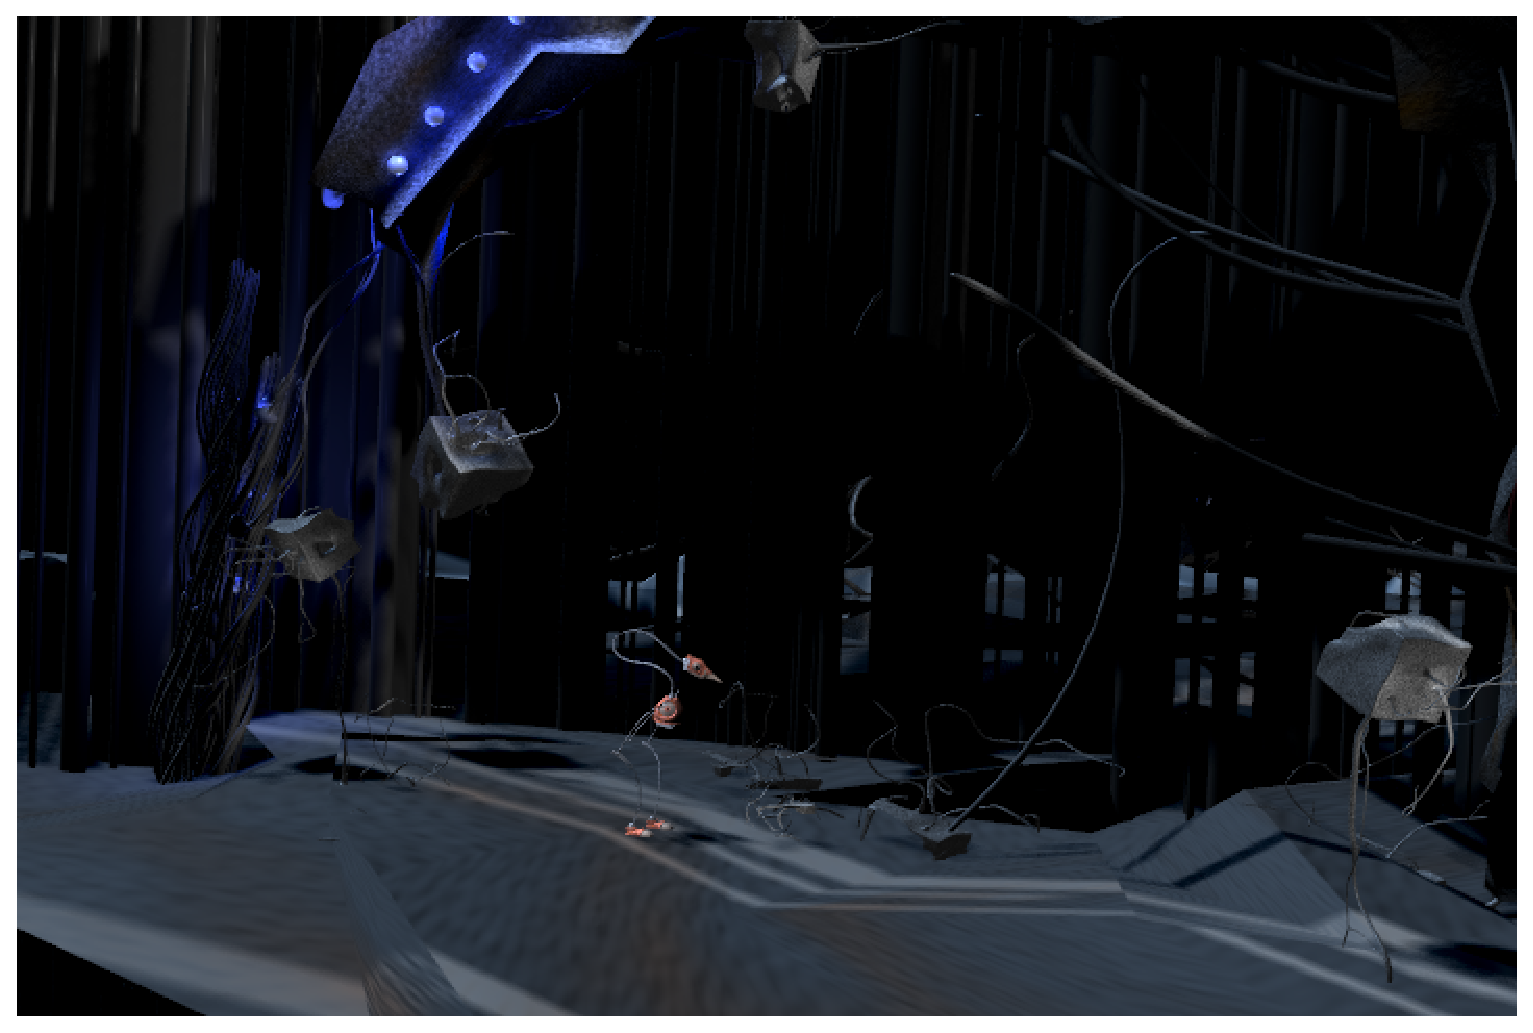
\psfig{file=compression/blender-background1-frame5.eps,width=1.9in}
\vspace{2pt}
\end{minipage}
\begin{minipage}{0.3\textwidth}
\centering

\psfig{file=compression/blender-foreground2-frame5.eps,width=1.9in}
\vspace{2pt}
\end{minipage}
\begin{minipage}{0.3\textwidth}
\centering
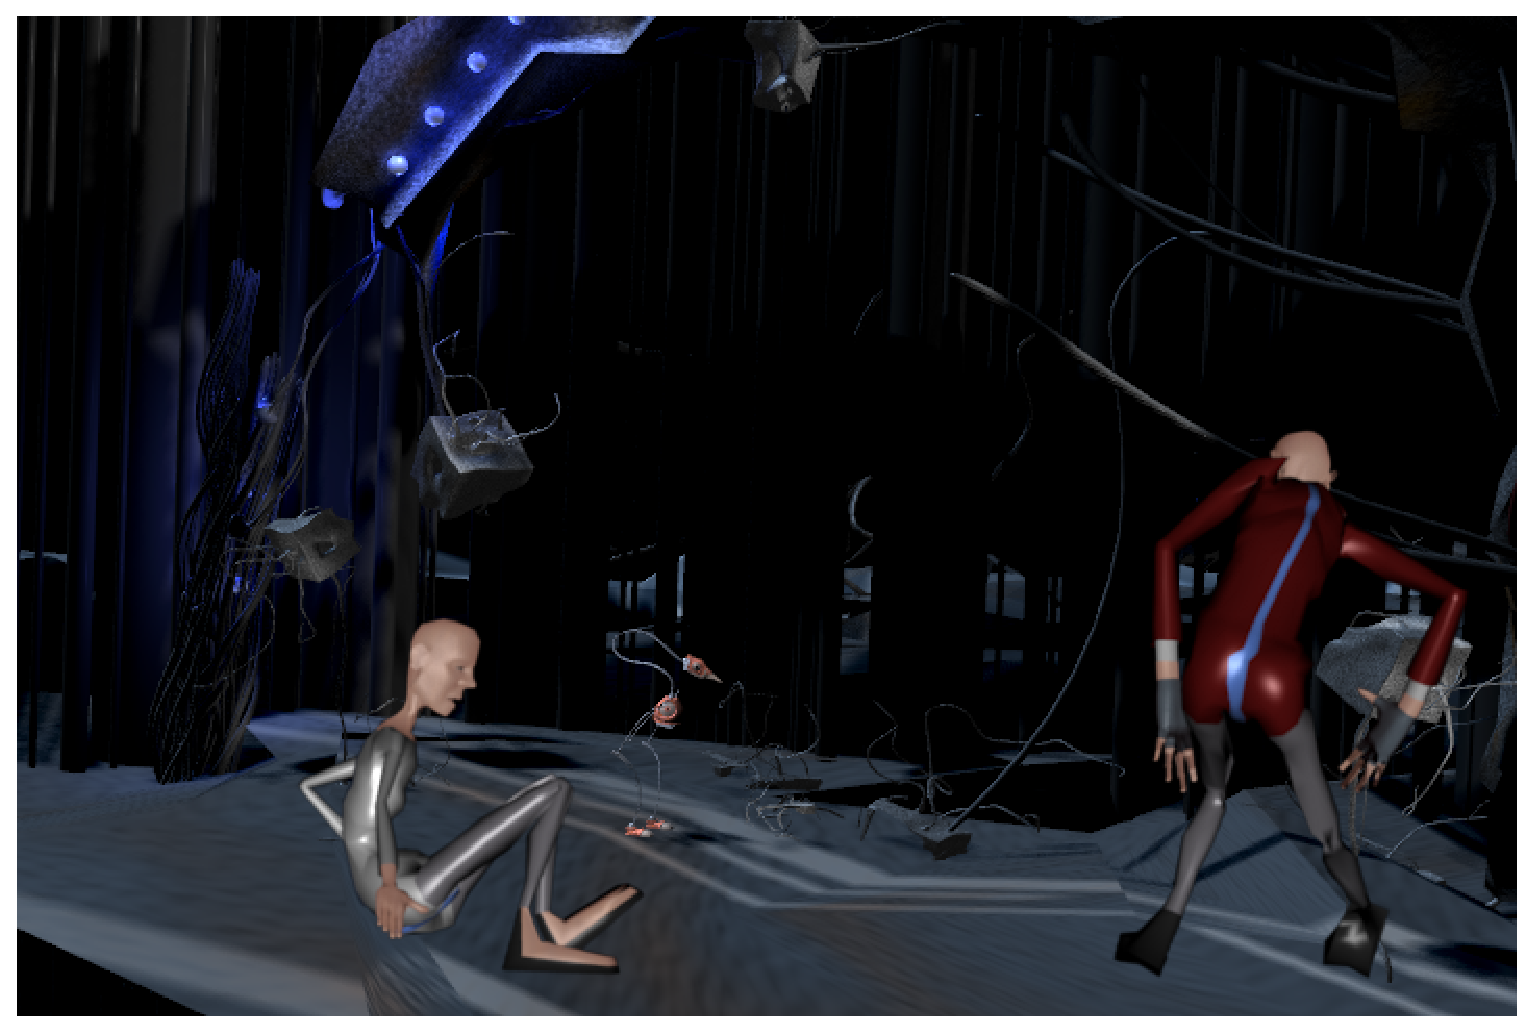
\psfig{file=compression/blender-composite-frame5.eps,width=1.9in}
\vspace{2pt}
\end{minipage}

{\small ~~~~~~~~~~~anim-scene1~~~~~~~~~~~~~~+~~~~~~~~~~~~~anim-character2~~~~~~~~~~~=~~~~~~~~~~~~~video composite~~~~~~~}

\begin{center}
\vspace{-3pt}
(a) Computer animation composite (alpha-under)
\end{center} \vspace{12pt}

\begin{minipage}{0.3\textwidth}
\centering

\psfig{file=compression/digvid-background1.eps,width=1.9in}
\vspace{2pt}
\end{minipage}
\begin{minipage}{0.3\textwidth}
\centering
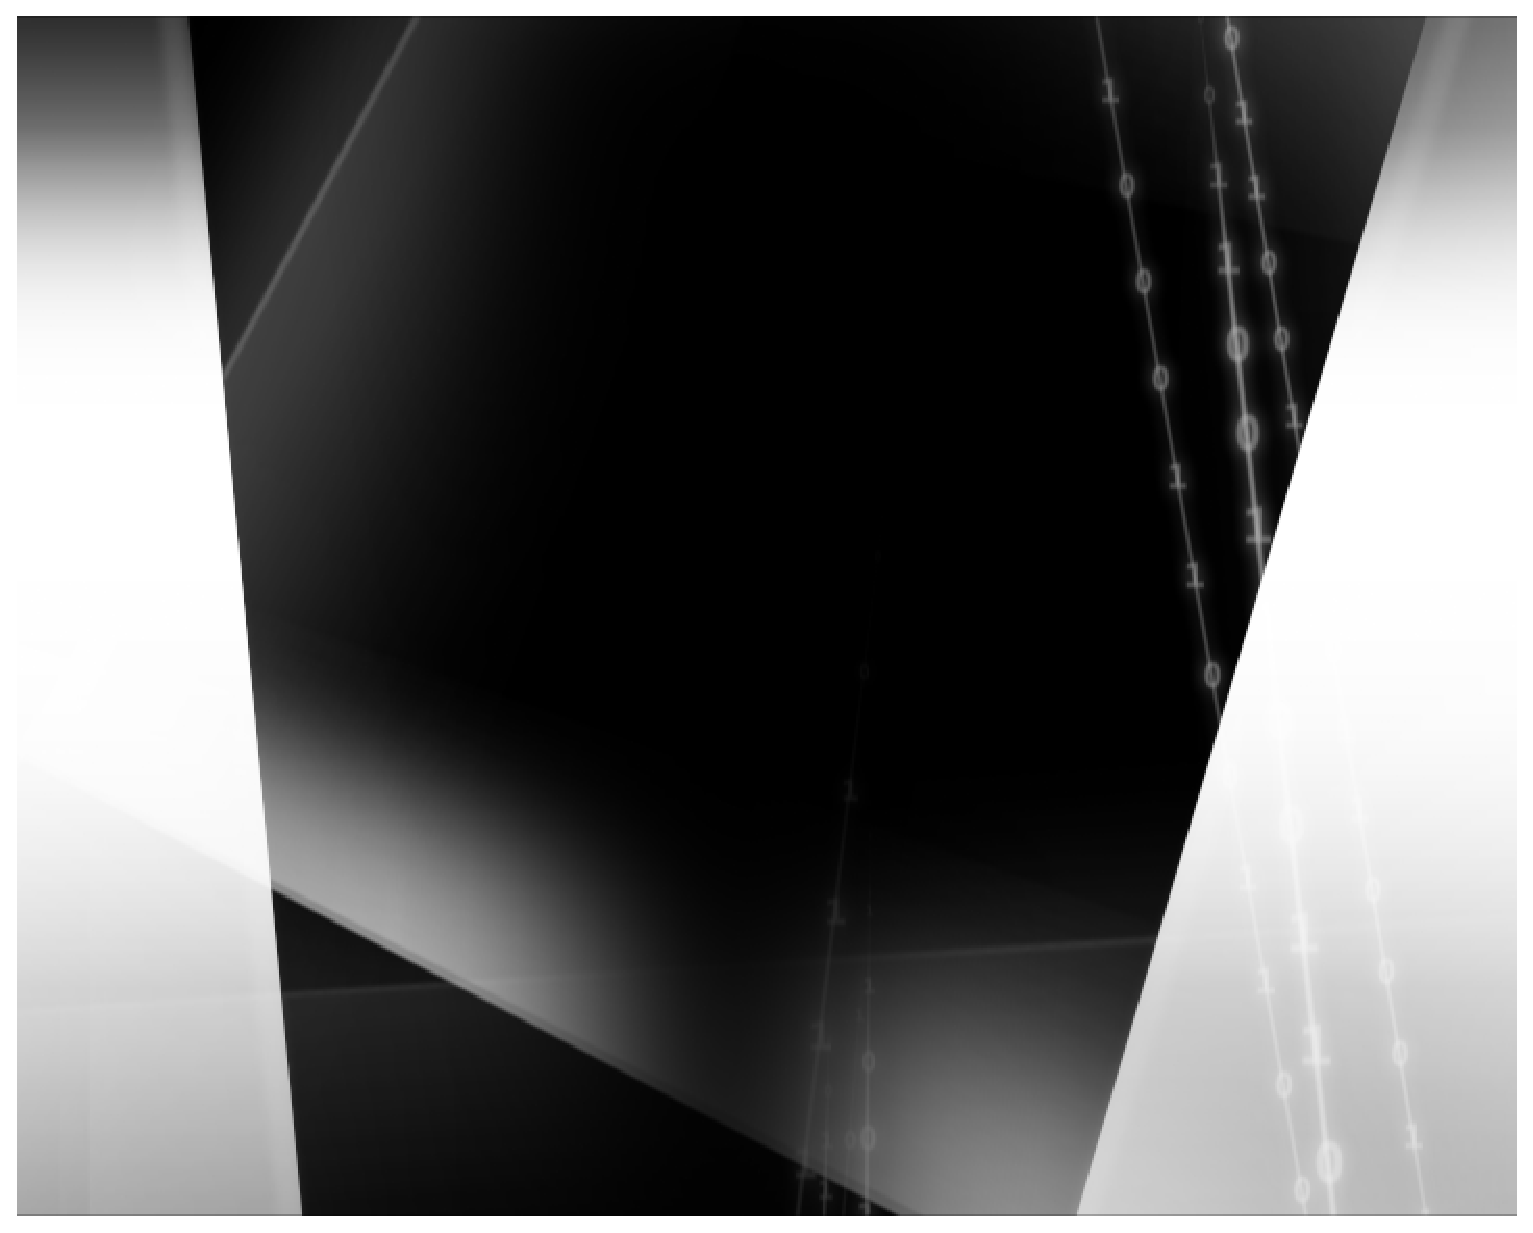
\psfig{file=compression/digvid-matte1-frame.eps,width=1.9in}
\vspace{2pt}
\end{minipage}
\begin{minipage}{0.3\textwidth}
\centering

\psfig{file=compression/digvid-composite.eps,width=1.9in}
\vspace{2pt}
\end{minipage}

{\small ~~~digvid-background1~~~~~~~~~~+~~~~~~~~~~~~digvid-matte-frame~~~~~~~~=~~~~~~~~~~~~~video composite~~~~~~~}

\begin{center}
\vspace{-3pt}
(b) Digital television composite (multiply)
\end{center}
\vspace{-3pt}
\caption{Examples of video compositing operations.\protect\label{fig:videos}}
\end{figure}

\begin{table*}[t]
\centering

\psfig{file=compression/table-composite-speedup.eps,width=5.8in}
\caption{Results for composite transformations.
\protect\label{tab:composite-speedup}}
\end{table*}

Our optimized configuration operates in the compressed domain.
Outside of the auto-generated plugin, we patched three frame-copy
operations in
% actually four frame-copy operations, though one of them is a no-op
the Blender source code to copy only the compressed frame data rather
than the full frame dimensions.

\subsubsection{Results}

Full results for the compositing operations appear in
Table~\ref{tab:composite-speedup}.  Figure~\ref{fig:composite-speedup}
illustrates the speedups, which range from 1.1x to 32x.  As in the
case of the pixel transformations, the speedups are closely correlated
with the compression factor of the resulting videos, a relationship
depicted in Figure~\ref{fig:speedup-scatter}.  The highly-compressed
screencasts enjoy the largest speedups (20x-32x), the computer
animations have intermediate speedups (5x-9x), while the digital
television content has negligible speedups (1.1x-1.4x).  Overall, the
speedups on video compositing (median = 6.6x) are lower than the pixel
transformations (median = 17x); this is because the compression
achieved on composite videos is roughly proportional to the minimum
compression across the two input files.

\begin{figure}[t]
\centering
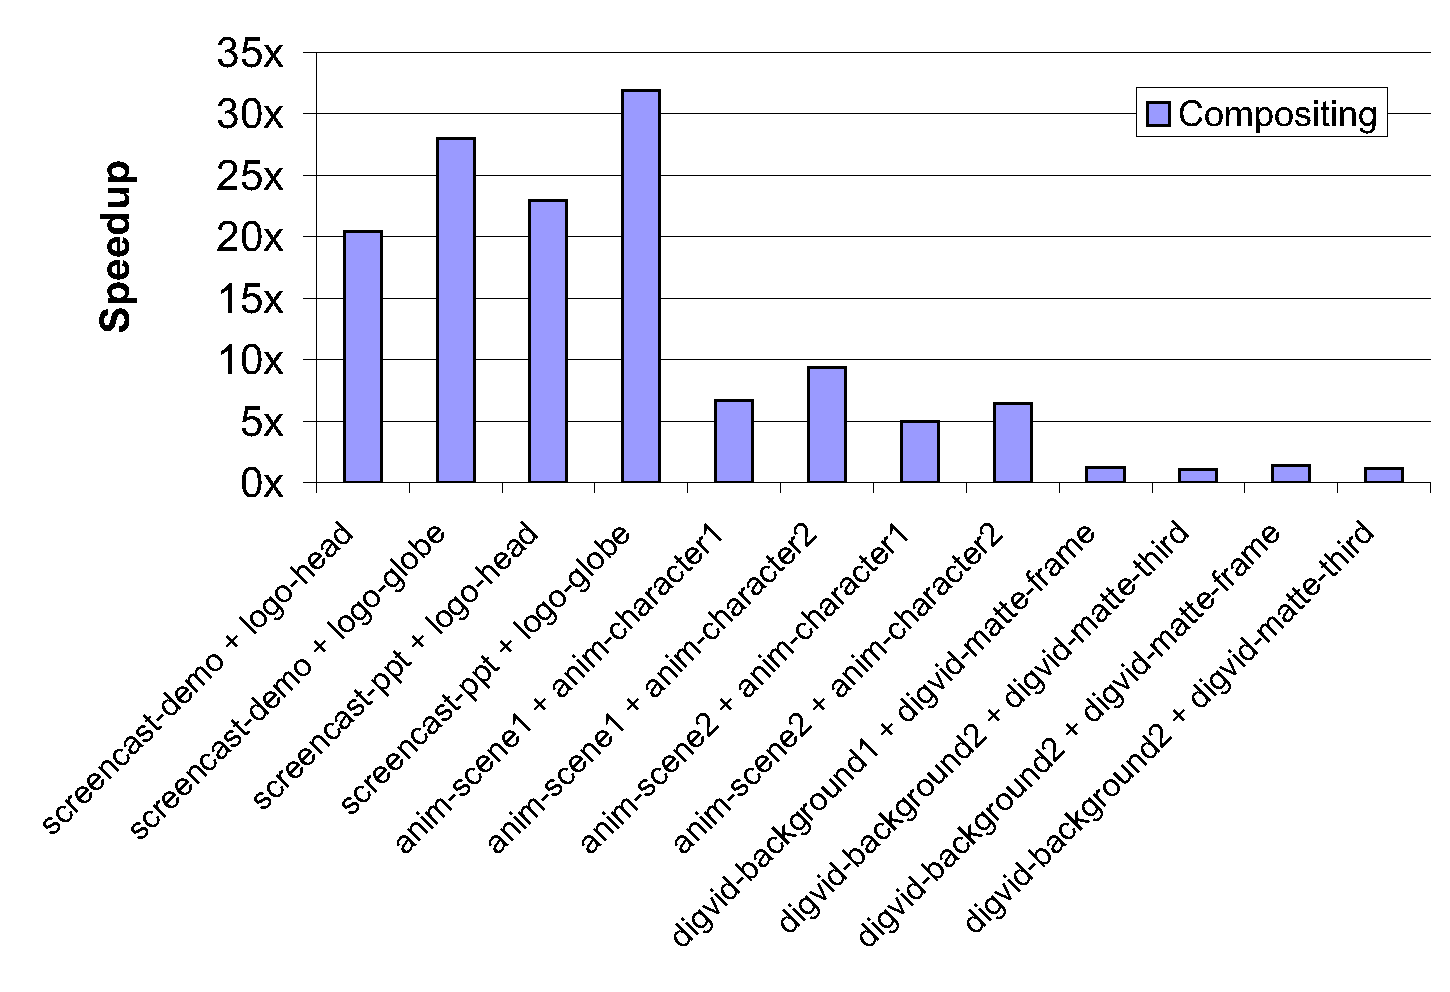
\psfig{file=compression/graph-speedup-composite.eps,width=4.355in}
\caption{Speedup on composite transformations.
\protect\label{fig:composite-speedup}}
\end{figure}

As for the pixel transformations, the composite videos produced by the
compressed processing technique would sometimes benefit from an
additional re-compression stage.  The last three columns in
Table~\ref{tab:composite-speedup} quantify this benefit by comparing
the compression factors achieved by compressed processing and normal
processing (including a re-compression step).  For screencasts and
computer animations, compressed processing preserves a sizable
compression factor (7.7x-44x), though the full re-compression can
further reduce file sizes by 1.2x to 1.6x.  For digital television,
the matting operations introduce a large amount of redundancy (black
regions), thereby enabling the re-compression stage to shrink the file
by 1.8x to 5.4x over the compressed processing technique.

Even if the composite transformation does not introduce any new
redundancy in the video, the compressed processing technique may
increase file sizes by ignoring a specific kind of redundancy in the
inputs.  Suppose that in the first frame, both inputs are 100\% black,
while in the second frame, one input is 100\% black and the other is
100\% white.  If the inputs are averaged, the second frame of output
will be 100\% gray and can be run-length encoded within the frame.
However, because the inputs have different kinds of redundancy on the
second frame (one is inter-frame, the other is intra-frame), the
technique is unable to detect the intra-frame redundancy in the output
and will instead produce N distinct pixels (all of them gray).  We
believe that this effect is small in practice, though we have yet to
quantify its impact in relation to the new redundancy introduced by a
transformation.  Future work will explore alternate data structures
for the compressed processing technique that may be able to preserve
this redundancy with low overhead.

\section{Related Work}
\label{sec:related}

Several other researchers have pursued the idea of operating directly
on compressed data formats.  The novelty of our work is two-fold:
first, in its focus on lossless compression formats, and second, in
its ability to map a flexible stream program, rather than a single
predefined operation, into the compressed domain.

Most of the previous work on mapping algorithms into the compressed
domain has focused on formats such as JPEG that utilize a Discrete
Cosine Transform (DCT) to achieve spatial
compression~\cite{smith98,dorai00,dugad01,feng03,mukherjee02,nang00,shen96,shen96b,shen98,smith96b,vasudev98}.
This task requires a different analysis, with particular attention
given to details such as the blocked decomposition of the image,
quantization of DCT coefficients, zig-zag ordering, and so-on.
Because there is also a run-length encoding stage in JPEG, our current
technique might find some application there; however, it appears that
techniques designed for JPEG have limited application to formats such
as LZ77.  
%Also, we are unaware of any previous methodology for
%translating a generic program to operate on compressed data; previous
%efforts have mapped each algorithm in a manual and ad-hoc way.

There has been some interest in performing compressed processing on
lossless encodings of black-and-white images.  Shoji presents the pxy
format for performing transpose and other affine
operations~\cite{shoji95}; the memory behavior of the technique was
later improved by Misra et al.~\cite{misra99}.  
%As described in
%Section~\ref{sec:formats}, the 
The pxy format lists the $(x,y)$ coordinate pairs at which a
black-and-white image changes color during a horizontal scan.  As
illustrated in Figure~\ref{fig:sj-example}, our technique can also
preserve a certain amount of compression during a transpose, though we
may achieve lesser compression than the pxy format due to our
one-dimensional view of the data.

Researchers have also considered the problem of pattern matching on
compressed text.  A randomized algorithm has been developed for
LZ77~\cite{farach98matching} while deterministic strategies exist for
LZ78 and LZW~\cite{navarro03regular,navarro05lzgrep}.  These solutions
are specialized to searching text; they do not apply to our
transformations, and our technique does not apply to theirs.

In the realm of programming languages, Swartz and Smith present RIVL,
a Resolution Independent Video Language~\cite{swartz95}.  The language
is used to describe a sequence of image transformations; this allows
the compiler to analyze the sequence and, via lazy evaluation, to
eliminate any operations that do not effect the final output.  Such a
technique is complementary to ours and could also be implemented using
StreamIt as the source language.

\section{Future Work}
\label{sec:future}

%% First, as the current transformation has the potential to increase the
%% size of the file, we plan to explore lightweight techniques for
%% re-compressing a data stream that is already partially compressed.
%% This should be straightforward in the case of Apple Animation; for
%% example, a run-length encoded unit can be extended without needing to
%% be rediscovered.

There remain rich areas for future work in computing on compressed
data.  First, the compressed processing technique can be applied far
beyond the current focus.  In its current form, the technique could be
evaluated on video operations such as thresholding, color depth
reduction, sepia toning, saturation adjustment, and color replacement.
With minor extensions, the technique can support video operations such
as cropping, padding, histograms, image flipping, sharpening, and
blurring.  The technique may also have applications in an embedded
setting, where it could offer power savings---for example, in
processing the RAW data format within digital cameras.  It may even be
possible to do sparse matrix operations using the technique; in
addition to compressing the locations of the zero elements, LZ77 would
also compress repetitive patterns in the non-zero elements.

Research is also underway to apply a similar technique to lossy,
DCT-based compression formats.  The streaming model of computation
also offers key advantages in this domain, as neighboring actors that
compute linear functions can be algebraically simplified at compile
time~\cite{aalamb}.  For example, a JPEG transcoder typically performs
an iDCT (during decompression), followed by the user's transformation,
followed by a DCT (during compression).  If the user's transformation
is also linear (e.g., color inversion) then all three stages can be
automatically collapsed, thereby eliminating the decompression and
re-compression steps.  Preliminary experiments in this direction
indicate speedups upwards of 10x.  By extending the framework to
multiple compression formats, users will be able to write their
transformations once, in a high-level language, and rely on the
compiler to map the computations to each of the compressed domains.

\section{Conclusions}
\label{sec:conclusions}

%% Many of the applications that will drive the next generation of
%% computing systems---digital video editing, computer vision, computer
%% graphics and animation---operate on image and video formats that are
%% universally stored in compressed data formats.  

In order to accelerate operations on compressible data, this paper
presents a general technique for translating stream programs into the
compressed domain.  Given a natural program that operates on
uncompressed data, our transformation outputs a program that directly
operates on the compressed data format.  We support lossless
compression formats based on LZ77.  In the general case, the
transformed program may need to partially decompress the data to
perform the computation, though this decompression is minimized
throughout the process and significant compression ratios are
preserved without resorting to an explicit re-compression step.

%% While we formulated our transformation in terms of the cyclo-static
%% dataflow model, the techniques can be applied within other functional
%% and general-purpose languages so long as the right information is
%% available and certain constraints are satisfied.  The transformation
%% relies on a regular pattern of data access; we use a streaming
%% abstraction, but structured iteration over arrays could also suffice.
%% We rely on static data rates in actors, which could also be expressed
%% as functions with a fixed number of arguments and return values.
%% Actors (functions) must be pure, without side effects or unresolvable
%% dependences on potentially mutable data.  While these properties are
%% intrinsic to a language such as StreamIt, they also come naturally in
%% most functional languages and may be adaptable to general-purpose
%% languages in the form of a runtime library with a restricted API.

We implemented some of our transformations in the StreamIt compiler
and demonstrated excellent speedups.  Across a suite of 12 videos in
Apple Animation format, computing directly on compressed data offers a
speedup roughly proportional to the compression ratio.  For pixel
transformations (brightness, contrast, inverse) speedups range from
2.5x to 471x, with a median of 17x; for video compositing operations
(overlays and mattes) speedups range from 1.1x to 32x, with a median
of 6.6x.  While previous researchers have used special-purpose
compressed processing techniques to obtain speedups on lossy,
DCT-based codecs, we are unaware of a comparable demonstration for
lossless video compression.  As digital films and animated features
have embraced lossless formats for the editing process, the speedups
obtained may have practical value.

% SPEEDUPS
\newcommand{\meanspeedup}[0]{2.78x}

\startchapter{Migrating Legacy C Programs to a Streaming Representation}
\label{chap:profiling}

This chapter stands independently of the StreamIt project.  Rather
than starting with a stream programming language, we consider the
problem of starting with a legacy C application and migrating the code
to a streaming representation.  To address this problem, we equip the
programmer with a simple set of annotations (indicating possible
filter boundaries) and a dynamic analysis that tracks all
communication across those boundaries.  Our analysis outputs a stream
graph of the application as well as a set of macros for (unsoundly)
parallelizing the program and communicating the data needed.

Our analysis is unsound because it is based on a fixed set of dynamic
traces, rather than a conservative static analysis.  However, we argue
that this unsoundness enables us to provide programmers with more
information, that is ultimately more useful, than can be expected from
a static analysis.  We apply our methodology to six case studies,
including MPEG-2 decoding, MP3 decoding, GMTI radar processing, and
three SPEC benchmarks.  Our analysis extracts a useful block diagram
for each application, facilitating a translation to StreamIt and other
stream languages.  In addition, the parallelized versions run
correctly (given appropriate training inputs) and offer a
{\meanspeedup} mean speedup on a 4-core machine.

\section{Introduction}

While adopting a stream programming model is an attractive approach
for improving the performance of future applications, one of the
drawbacks of relying on a new programming model is that it does not
immediately address the vast quantities of legacy code that have
already been written in other languages.  There are 310 billion lines
of legacy code in industry today, and 75-80\% of the typical IT budget
is spent maintaining legacy systems~\cite{legacy}.  While much of this
code is amenable to streaming, the process of migrating the code to a
streaming representation is an arduous and time-consuming process.
The most important resources that could help with the translation --
such as the original author of the code, or the high-level design
documents that guided its implementation -- are often unavailable.
Thus, a fresh programmer is left with the daunting task of obtaining
an in-depth understanding of all the program modules, the dependences
between them, and the possibilities for safely extracting parallelism.

While there have been many efforts to automatically parallelize legacy
codes, few of them have focused on the pipeline parallelism that is
characteristic of the streaming domain.  It is even difficult to
express pipeline parallelism in a traditional programming model.  This
is in stark contrast to task parallelism, which is naturally supported
by threads, as well as data parallelism, which is supported by
dialects such as OpenMP.  The only efforts to exploit pipeline
parallelism in C programs have been very fine-grained, partitioning
individual instructions across processing
cores~\cite{ottoni05decoupled}.  Such fine-grained communication is
inefficient on commodity machines and demands new hardware
support~\cite{ottoni05decoupled,rangan04array}.  While a
coarse-grained partitioning is more desirable, it is difficult to
achieve at compile time due to the obscured data dependences in C;
constructs such as pointer arithmetic, function pointers, and circular
buffers (with modulo operations) make it nearly impossible to extract
coarse-grained parallelism from realistic C programs.

%Each pipeline stage can
%progress independently, so long as there is input data available from
%the previous stage.

%% Pipeline parallelism is an important abstraction, suitable to both new
%% and existing programs, that all parallel programmers should have at
%% their disposal.  Firstly, pipeline parallelism is often lurking in
%% otherwise sequential codes.  Loops with carried dependences can admit
%% a pipeline-parallel mapping (the dependence being carried by a single
%% pipeline stage) even though a data-parallel mapping is impossible.
%% Secondly, pipeline parallelism can be more efficient than data
%% parallelism due to improved instruction and data locality within each
%% pipeline stage, as well as point-to-point communication between cores
%% (there is no global scatter/gather).  Pipeline parallelism also offers
%% appeals over task parallelism, as all shared data can be communicated
%% in a deterministic producer/consumer style, eliminating the
%% possibility of data races.

In this chapter, we overcome the traditional barriers in exploiting
coarse-grained pipeline parallelism by embracing an {\it unsound}
program transformation.  Our key insight is that, for stream programs,
the data communicated across pipeline-parallel stages is stable
throughout the lifetime of the program.  No matter how obfuscated the
C implementation appears, the heart of the algorithm is following a
regular communication pattern.  For this reason, it is unnecessary to
undertake a heroic static analysis; we need only observe the
communication pattern at the beginning of execution, and then
``safely'' infer that it will remain constant throughout the rest of
execution (and perhaps other executions).

%then apply that pattern as the basis for
%parallelism in the remainder of the execution (and perhaps other
%executions).

As depicted in Figure~\ref{fig:overview}, our analysis does exactly
that.  We allow the programmer to naturally specify the boundaries of
pipeline partitions, and then we record all communication across those
boundaries during a training run.  The communication trace is emitted
as a stream graph that reflects the high-level structure of the
algorithm (aiding a possible translation to StreamIt), as well as a
list of producer/consumer statements that can be used to trace down
problematic dependences.  The programmer never needs to worry about
providing a ``correct'' partitioning; if there is no parallelism
between the suggested partitions, it will result in cycles in the
stream graph.  If the programmer is satisfied with the parallelism in
the graph, he recompiles the annotated program against a set of macros
that are emitted by our analysis tool.  These macros serve to fork
each partition into its own process and to communicate the recorded
locations using pipes between processes.

\begin{figure}[t]
%% \newlength{\myoffset}
%% \setlength{\myoffset}{-\textwidth}
%% \addtolength{\myoffset}{\columnwidth}
%% \hspace{\myoffset}
\hspace{-0.25in}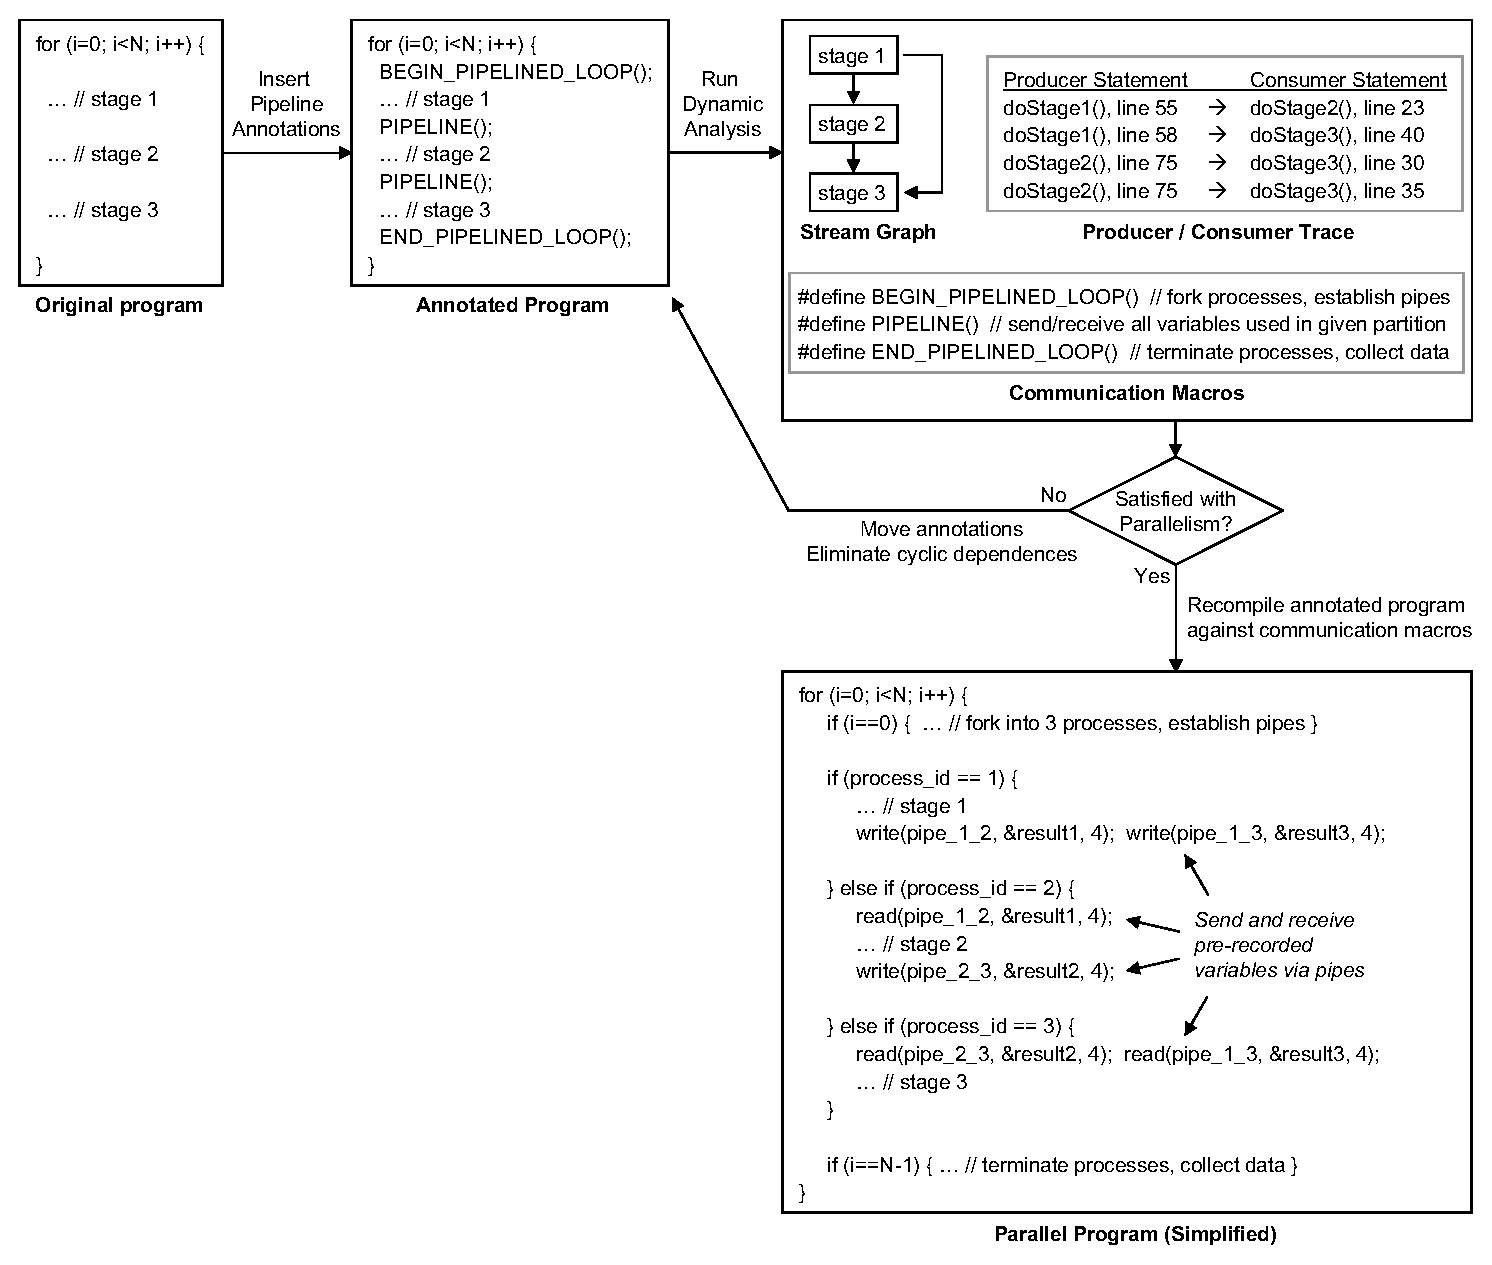
\psfig{file=profiling/intro-overview.eps,width=7in}
\vspace{-18pt}
\caption{Overview of our approach.\protect\label{fig:overview}}
\vspace{-6pt}
\end{figure}

Though our transformation is grossly unsound, we argue that it is
quite practical within the domain of streaming applications.  Because
pipeline parallelism is deterministic, any incorrect transformations
incurred by our technique can be identified via traditional testing
methods, and failed tests can be fixed by adding the corresponding
input to our training set.  Further, the communication trace provided
by our analysis is useful in aiding manual parallelization of the code
-- a process which, after all, is only sound insofar as the
programmer's understanding of the system.  By improving the
programmer's understanding, we are also improving the soundness of the
current best-practice for parallelizing legacy C applications.

We have applied our methodology to six case studies: MPEG-2 decoding,
MP3 decoding, GMTI radar processing, and three SPEC benchmarks.  Our
tool was effective at parallelizing the programs, providing a mean
speedup of {\meanspeedup} on a four-core architecture.  Despite the
potential unsoundness of the tool, our transformations correctly
decoded ten popular videos from YouTube, ten audio tracks from
MP3.com, and the complete test inputs for GMTI and SPEC benchmarks.
At the same time, we did identify specific combinations of training
and testing data (for MP3) that lead to erroneous results.  Thus, it
is important to maximize the coverage of the training set and to apply
the technique in concert with a rigorous testing framework.

The remainder of this chapter is organized as follows.  In
Section~\ref{sec:stability}, we show that stream programs have a
stable communication pattern.  Communication observed at the start of
execution is often preserved throughout the program lifetime, as well
as other executions.  Section~\ref{sec:workflow} describes our dynamic
analysis tool and programmer methodology to iteratively extract stream
parallelism from C programs.  Section~\ref{sec:parallelization}
describes the implementation of the tool using the Valgrind
infrastructure.  Section~\ref{sec:results} is devoted to our case
studies, including performance results and the experience gained
during parallelization.  The remaining sections present related work,
future work, and a chapter summary.

%% CONTRIBUTIONS
%%
%% \item We define a simple API for indicating potential pipeline
%%   parallelism in the program.  Comparable to threads for task
%%   parallelism or OpenMP for data parallelism, this API serves as a
%%   fundamental abstraction for pipeline parallelism
%%   (Section~\ref{sec:workflow}).
%%
%% \item We present a dynamic analysis tool, built on top of Valgrind,
%%   for tracking producer/consumer relationships between coarse-grained
%%   program partitions.  The tool outputs a stream graph of the
%%   application, which validates or refutes the parallelism suggested by
%%   the programmer.  It also provides a detailed statement-level trace
%%   and a set of macros for automatic parallelization
%%   (Sections~\ref{sec:workflow}-\ref{sec:parallelization}).
%%
%% \item We apply our methodology to six case studies, encompassing
%%   MPEG-2 decoding, MP3 decoding, GMTI radar processing, and three SPEC
%%   benchmarks.  We extract meaningful stream graphs of each
%%   application, and achieve a {\meanspeedup} mean speedup on a 4-core
%%   architecture (Section~\ref{sec:results}).

%% \begin{figure*}[t]
%% \begin{center}
%% \hspace{0pt}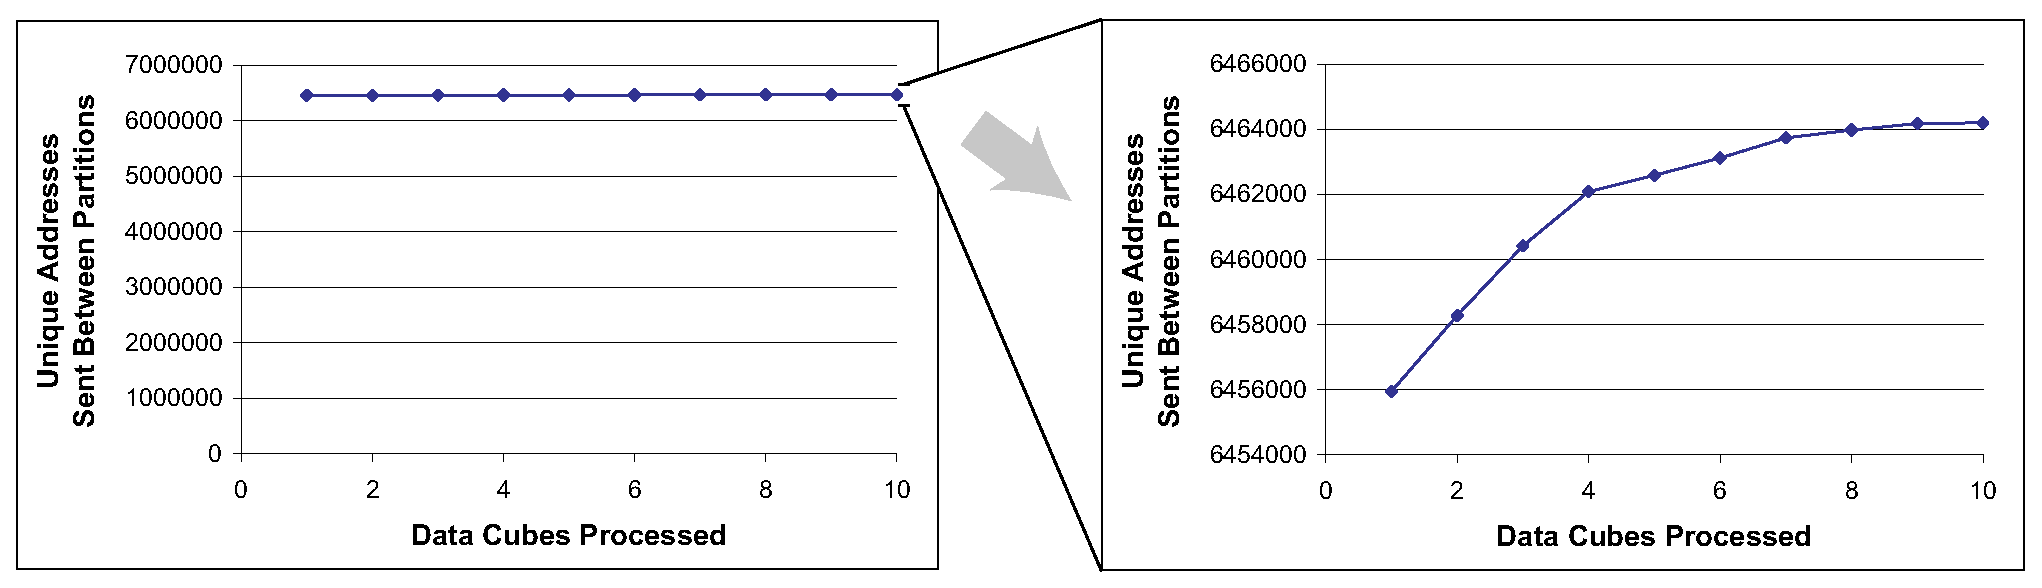
\psfig{file=profiling/gmti.eps,width=\textwidth}
%% \caption{Stability of streaming communication patterns for GMTI radar
%%   processing. See Figure~\ref{fig:gmti-graph} for a stream graph of
%%   the application.\protect\label{fig:gmti-stability}}
%% \end{center}
%% \end{figure*}

%% \begin{table*}[t]
%% \vspace{10pt}
%% \small
%% \begin{center}
%% \begin{tabular}{|l|l|l|l|}
%% \hline
%% {\bf Benchmark} & {\bf Training Input} & {\bf Testing Input} & {\bf Testing Output} \\ \hline
%% \parbox{0.8in}{~ \vspace{-3pt} \\ MPEG-2 \\ Decoding  ~\\ \vspace{-7pt}} &  First 10 frames of a local video & \parbox{1.9in}{~ \vspace{-3pt} \\ Top 10 short videos from YouTube\\ + user-supplied frame size ~ \\ \vspace{-7pt}} & 100\% correct\\ \hline
%% \parbox{0.8in}{~ \vspace{-3pt} \\ MP3 \\ Decoding  ~\\ \vspace{-7pt}} & First 3 samples of a local CD track & \parbox{1.9in}{~ \vspace{-3pt} \\ Top 10 downloads from mp3.com\\ (tens of thousands of samples) ~\\ \vspace{-7pt}} & 100\% correct \\ \hline
%% \parbox{0.8in}{~ \vspace{-3pt} \\ GMTI Radar \\ Processing  ~\\ \vspace{-7pt}} & \parbox{2in}{~ \vspace{-3pt} \\ First 10 data cubes of input + \\ user direction to fill sparse array ~\\ \vspace{-7pt}} & Rest of input (50 data cubes) & 100\% correct \\ \hline
%% \end{tabular}
%% \vspace{-6pt}

%% \caption{Stability of streaming communication patterns across
%%   different input files.  Using the tool and methodology described in
%%   this paper, we profiled the execution of three realistic streaming
%%   applications for a few iterations of a training input.  We used the
%%   observed communication trace to parallelize the program, executing
%%   each pipeline stage in a separate address space and relying on the
%%   trace to satisfy all of the data dependences.  Despite the short
%%   training period and the potential unsoundness of the technique, the
%%   trace was sufficiently stable to correctly execute unrelated input
%%   files (from YouTube and MP3.com) in a parallel
%%   context.\protect\label{tab:stability}}
%% \vspace{-6pt}
%% \end{center}
%% \end{table*}

\section{Stability of Stream Programs}
\label{sec:stability}

A dynamic analysis is most useful when the observed behavior is likely
to continue, both throughout the remainder of the current execution as
well as other executions (with other inputs).  Our hypothesis is that
stream programs exhibit very stable flows of data, enhancing the
reliability of dynamic analyses toward the point where they can be
trusted to validate otherwise-unsafe program transformations.  For the
purpose of our analysis, we consider a program to be {\it stable} if
there is a predictable set of memory dependences between pipeline
stages.  The boundaries between stages are specified by the programmer
using a simple set of annotations; the boundaries used for the
experiments in this section are illustrated by the stream graphs that
appear later (Figure~\ref{fig:mpeg2-mp3-graphs}).

\subsection*{Stability Within a Single Execution}

Our first experiment explores the stability of memory dependences
within a single program execution.  We profiled MPEG-2 and MP3
decoding using the most popular content from YouTube\footnote{YouTube
  videos were converted from Flash to MPEG-2 using ffmpeg and
  vixy.net.} and MP3.com; results appear in
Figures~\ref{fig:mpeg2-addresses} and~\ref{fig:mp3-addresses}.  These
graphs plot the cumulative number of unique addresses that are passed
between program partitions as execution proceeds.  The figures show
that after a few frames, the program has already performed a
communication for most of the addresses it will ever send between
pipeline stages.

In the case of MPEG-2, all of the address traces remain constant after
50 frames, and 8 out of 10 traces remain constant after 20 frames.
The videos converge at different rates in the beginning due to varying
parameters and frame types; for example, video 10 contains an
intra-coded frame where all other videos have a predictive-coded
frame, thereby delaying the use of predictive buffers in video 10.
Video 1 communicates more addresses than the others because it has a
larger frame size.

MP3 exhibits a similar stability property, though convergence is
slower for some audio tracks.  While half of the tracks exhibit their
complete communication pattern in the first 35 frames, the remaining
tracks exhibit a variable delay (up to 420 frames) in making the final
jump to the common communication envelope.  These jumps correspond to
elements of two parameter structures
% ({\tt III\_side\_info} and {\tt III\_scalefac}) 
which are toggled only upon encountering certain frame types.  Track
10 is an outlier because it starts with a few layer-1 frames, thus
delaying the primary (layer-3) communication and resulting in a higher
overall communication footprint.  The only other file to contain
layer-1 frames is track 9, resulting in a small address jump at
iteration 17,900 (not illustrated).

\begin{figure}[t]
\begin{minipage}{3.075in}
\hspace{-0.05in}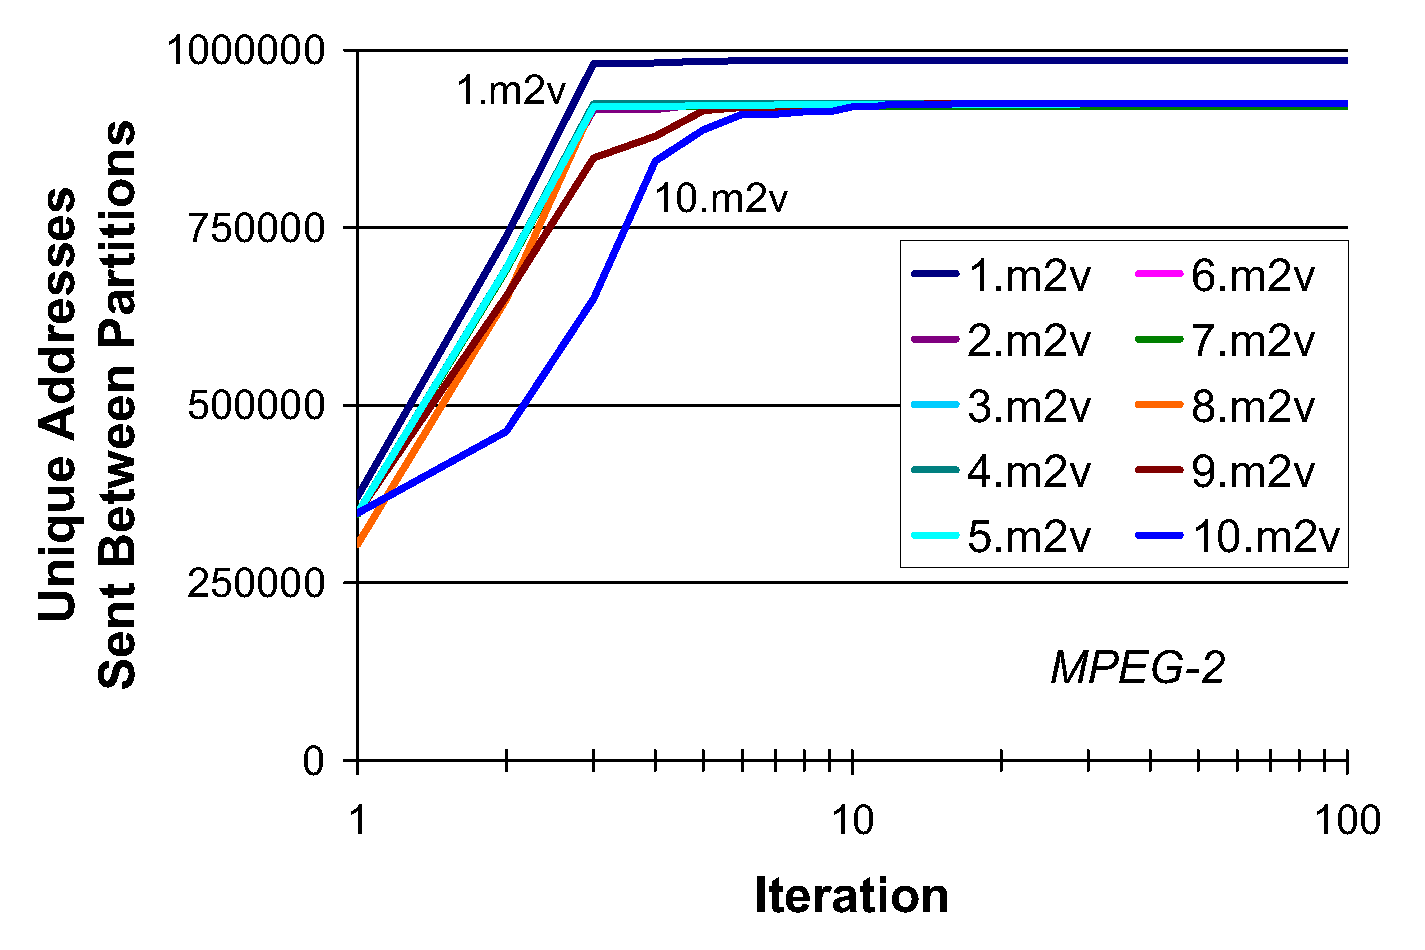
\psfig{file=profiling/mpeg2-addresses.eps,width=3.125in}
\vspace{-12pt}
\caption[Stability of streaming communication patterns for MPEG-2
  decoding.]{Stability of streaming communication patterns for MPEG-2
  decoding.  The decoder was monitored while processing the top 10
  short videos
% (25-35 seconds) 
from YouTube.  See Figure~\ref{fig:mpeg2-mp3-graphs}a for a stream
graph of the application.\protect\label{fig:mpeg2-addresses}}
\end{minipage}
\hspace{0.3in}
\begin{minipage}{3.02in}
\hspace{-0.05in}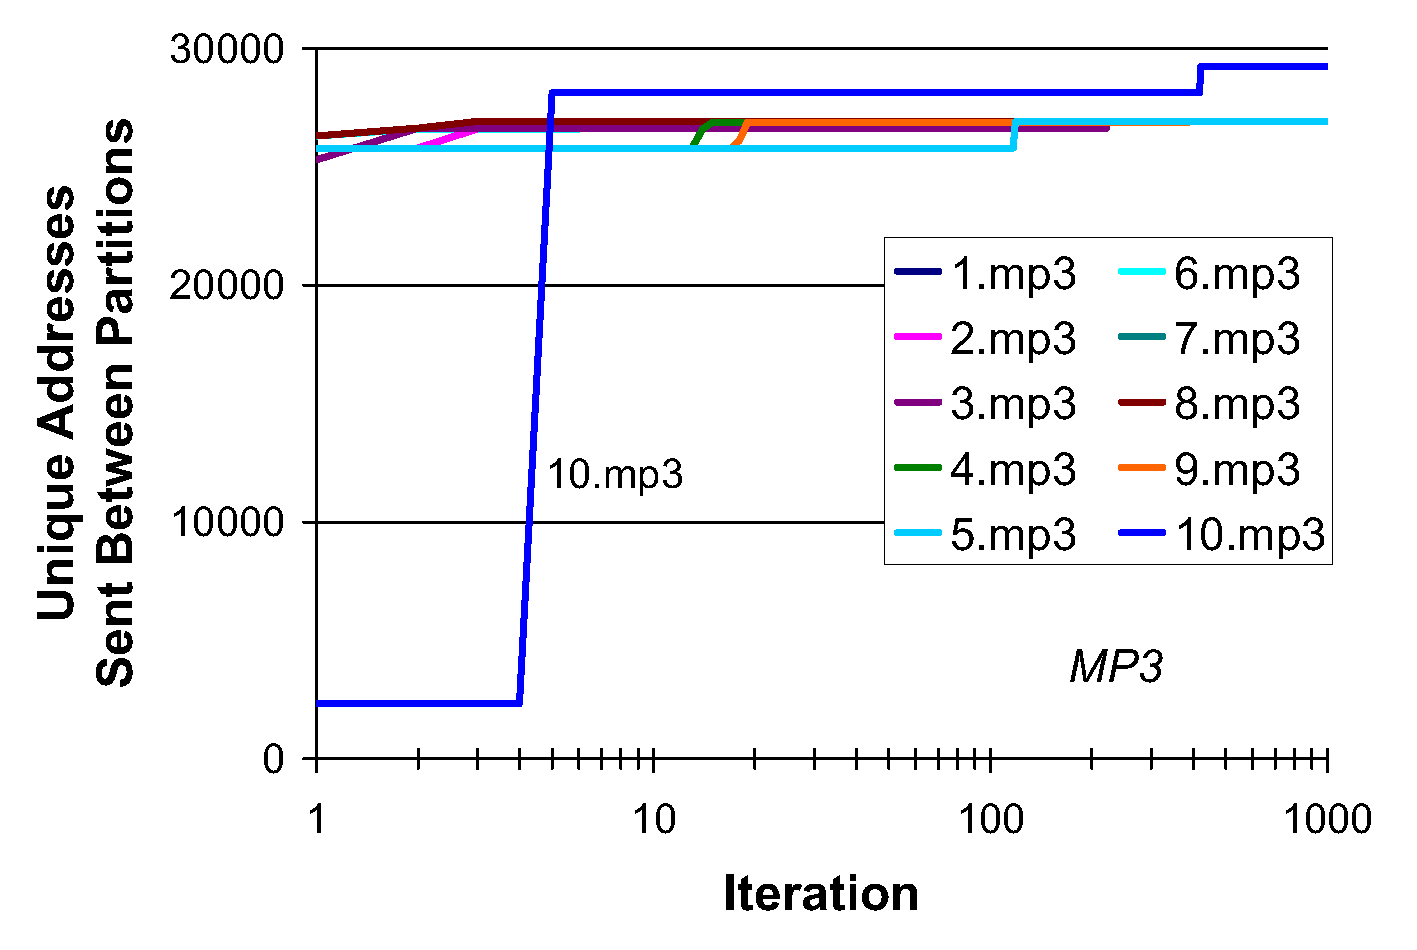
\psfig{file=profiling/mp3-addresses.eps,width=3.125in}
\vspace{-12pt}
\caption[Stability of streaming communication patterns for MP3
  decoding.]{Stability of streaming communication patterns for MP3
  decoding.  The decoder was monitored while processing the top 10
  tracks from MP3.com.  See Figure~\ref{fig:mpeg2-mp3-graphs}b for a
  stream graph of the application.  \protect\label{fig:mp3-addresses}}
\end{minipage}
\end{figure}

\begin{figure}[t]
\begin{minipage}{3.075in}

\psfig{file=profiling/mpeg2-matrix.eps,width=3.07in}
\vspace{-12pt}
\caption[Training needed for correct parallelization of
  MPEG-2.]{Minimum number of training iterations (frames) needed on
  each video in order to correctly decode the other videos.
  \protect\label{tab:mpeg2-matrix}}
\end{minipage}
\hspace{0.3in}
\begin{minipage}{3.02in}

\psfig{file=profiling/mp3-matrix.eps,width=3.07in}
\vspace{-12pt}
\caption[Training needed for correct parallelization of MP3.]{Minimum
  number of training iterations (frames) needed on each track in order
  to correctly decode the other tracks.
  \protect\label{tab:mp3-matrix}}
\end{minipage}
\end{figure}

It is important to note that there does exist a dynamic component to
these applications; however, the dynamism is contained within a single
pipeline stage.  For example, in MP3, there is a Huffman decoding step
that relies on a dynamically-allocated lookup tree.  Throughout the
program, the shape of the tree grows and shrinks and is manipulated on
the heap.  Using a static analysis, it is difficult to contain the
effects of such dynamic data structures; a conservative pointer or
shape analysis may conclude that the dynamism extends throughout the
entire program.  However, using a dynamic analysis, we are able to
observe the actual flow of data, ignoring the intra-node communication
and extracting the regular patterns that exist between partitions.

%% We also tracked the communication pattern for the GMTI radar tracker
%% for the single input included in its distribution (see
%% Figure~\ref{fig:gmti-stability}).  Unlike MP3 and MPEG-2, GMTI has a
%% slow and gradual increase in the data communicated across iterations.
%% The user of our tool inspected the addresses that were increasing and
%% found that an array was being read in a sparse pattern that was
%% gradually encompassing the entire data space.  Based on this
%% knowledge, the programmer instructed the tool to communicate the
%% entire array between partitions for the sake of the program
%% transformations.

%% The stability observed here could prove useful when doing a dynamic
%% optimization of streaming applications.  By profiling only the first
%% few iterations, one can observe the bulk of the data dependences
%% present in later iterations.

%While the outlying cases and lingering
%addresses may be important to catch, they may also be expendable, as
%we describe next.

\subsection*{Stability Across Different Executions}

The communication patterns observed while decoding one input file can
often extend to other inputs as well.  Figures \ref{tab:mpeg2-matrix}
and~\ref{tab:mp3-matrix} illustrate the minimum number iterations
(i.e., frames) that need to be profiled from one file in order to
enable correct parallel decoding of the other files.  In most cases, a
training set of five loop iterations is sufficient to infer an address
trace that correctly decodes the other inputs in their entirety.  The
exceptions are tracks 9 and 10 of MP3 decoding, which are the only two
files containing layer-1 frames; because they execute code that is
never reached by the other files, training on the other files is
insufficient to expose the full communication trace.  In addition,
track 9 is insufficient training for track 10, as the latter contains
an early CRC error that triggers a unique recovery procedure.  As each
of these hazards is caused by executing code that is untouched by the
training set, the runtime system could easily detect such cases (using
guards around untrained code) and revert to a sequential execution for
the iterations in question.  Rigorous testing practices that
incorporate code coverage metrics would also help to reduce the risk
of encountering unfamiliar code at runtime.

The ability to generalize short training runs across multiple
executions relies on two aspects of our methodology.  First, as
described later, we require the user to supply a symbolic size for
each dynamically-allocated variable; this allows MPEG-2 address traces
to apply across different frame sizes.  Second, we coarsen the
granularity of the trace to treat structure types and
dynamically-allocated segments as atomic units.  That is, whenever a
single element of such a structure is communicated between partitions,
the rest of the structure is communicated as well (so long as it does
not conflict with a local change in the target partition).  Such
coarsening increases the tolerance to small element-wise changes as
observed in later iterations of MPEG-2 and MP3.  However, it does not
trivialize the overall result, as coarsening is only needed for a
small fraction of communicated addresses (15\% for MP3 and dependent
on frame size for MPEG-2).
% to make this statement stronger, should actually measure the
% percentage of communicated VARIABLES, though I could not gather this
% number for MPEG-2 at the last minute.  (For large frame sizes, 97%
% of the data is malloc'd.)

% details:
% we need coarsening for: III_scalefac, III_side_info, and possibly (?) info
% we do not need for:
% ch, fr_ps, gr, hybridIn, hybridOut, is, pcm_sample, ro, sb, stereo
% 
% fr_ps is a struct but it would just as well not be, so not counting
% many more variables COULD have been communicated, but only these were

While we have focused on MPEG-2 and MP3 in this section, we observe
similar stability across our other benchmarks (GMTI, bzip2, parser,
and hmmer).  As described in Section~\ref{sec:results}, we profile
five iterations of a training file and (with minimal programmer
intervention) apply the trace to correctly execute a test file.

\section{Migration Methodology}
\label{sec:workflow}

We introduce a dynamic analysis tool that empowers the programmer in
migrating legacy C applications to a streaming representation.  Using
this tool, the programmer follows the workflow illustrated in
Figure~\ref{fig:overview}.  The first step is to identify the main
loop in the application, which is typically iterating over frames,
packets, or another long-running data source.  The programmer
annotates the start and end of this loop, as well as the boundaries
between the desired pipeline-parallel partitions.  The tool reports
the percentage of execution time spent in each pipeline stage in order
to help guide the placement of pipeline boundaries.

In our current implementation, there are some restrictions on the
placement of the partition boundaries.  All boundaries must appear
within the loop body itself, rather than within a nested loop, within
nested control flow, or as part of another function (this is an
artifact of using macros to implement the parallelism).  The
programmer may work around these restrictions by performing loop
distribution or function inlining.  Also, though both {\tt for} loops
and {\tt while} loops are supported, there cannot be any {\tt break}
or {\tt continue} statements within the loop; such statements
implicitly alter the control flow in all of the partitions, an effect
that is difficult to trace in our dynamic analysis.  If such
statements appear in the original code, the programmer needs to
convert them to a series of {\tt if} statements, which our tool will
properly handle.

Once a loop has been annotated with partition boundaries, the
programmer selects a set of training inputs and runs our dynamic
analysis to trace the communication pattern.  The tool outputs a
stream graph, a list of producer/consumer statements, and a set of
communication macros for automatically running the code in parallel.

\begin{figure}[t!]
\centering
% 338 pix wide
\hspace{0in}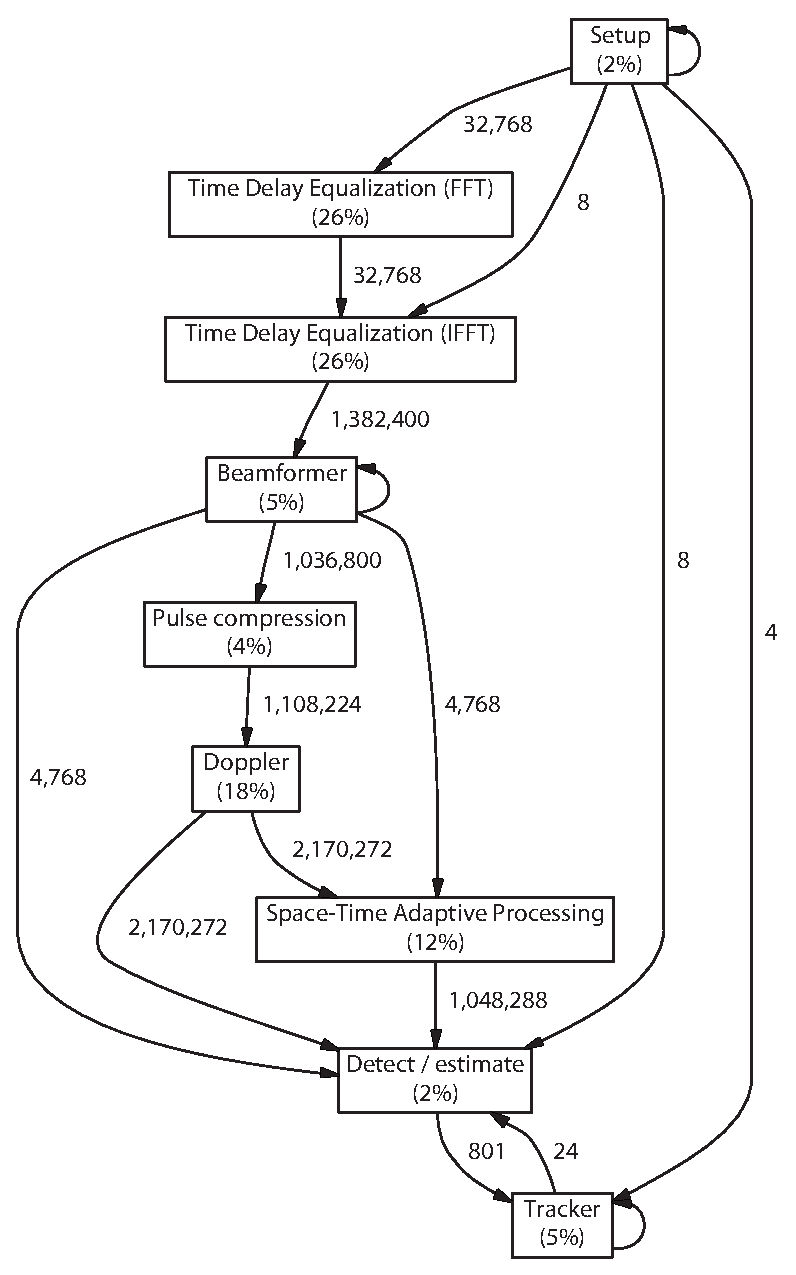
\psfig{file=profiling/gmti-opt.eps,width=2.9in}
\caption[Stream graph for GMTI, as extracted using our tool.]{Stream
  graph for GMTI, as extracted using our tool.  Nodes are annotated
  with their computation requirements, and edges are labeled with the
  number of bytes transferred per steady-state
  iteration.\protect\label{fig:gmti-graph-tool}}
\end{figure}

\begin{figure}[t!]
% to fill up this page
\vspace{6pt}
\centering
\hspace{0in}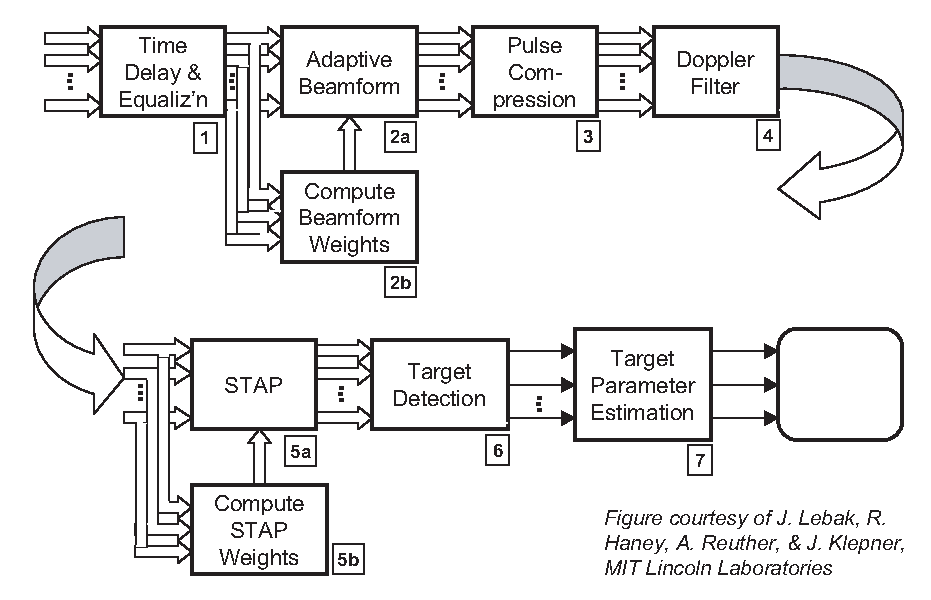
\psfig{file=profiling/gmti-spec.eps,width=3.3in}
\caption[Stream graph for GMTI, as it appears in the GMTI
  specification.]{Stream graph for GMTI, as it appears in the GMTI
  specification~\protect\cite{reuther03gmti}.\protect\label{fig:gmti-graph-spec}}
\vspace{-6pt}
\end{figure}

An example stream graph for GMTI radar processing appears in
Figure~\ref{fig:gmti-graph-tool}.  The graph extracted by our tool is
very similar to the block diagram from the GMTI specification, which
appears in Figure~\ref{fig:gmti-graph-spec}.  Our graph contains some
additional edges that are not depicted in the specification; these
represent communication of minor flags rather than the steady-state
dataflow.  Edges flowing from a node back unto itself (e.g., in Setup,
Beamformer, and Tracker) indicate mutable state that is retained
across iterations of the main loop.  Nodes without such dependences
are stateless with respect to the main loop, and the programmer may
choose to execute them in a data-parallel manner (see below).
% (There
%may also be more fine-grained data parallelism lurking in stateful
%nodes, due to nested loops within those nodes.)  
Overall, the tight correspondence between our extracted stream graph
and the original specification demonstrates that the tool can
effectively capture the underlying communication patterns, assisting
the programmer in understanding the opportunities and constraints for
parallelization.

Many nodes in a streaming application are suitable to data
parallelism, in which multiple loop iterations are processed in
parallel by separate instances of the node.  Such nodes are
immediately visible in the stream graph, as they lack a carried
dependence\footnote{In some cases, nodes with carried dependences on
  an outer loop can still be data-parallelized on an inner loop.  We
  perform such a transformation in MP3, though it is not fully
  automatic.} (i.e., a self-directed edge).  Our tool offers natural
support for exploiting data parallelism: the user simply provides an
extra argument to the {\tt PIPELINE} annotation, specifying the number
of ways that the following stage should be replicated (see
Figure~\ref{fig:data-parallelism}).  While this annotation does not
affect the profiler output, it is incorporated by the runtime system
to implement the intended parallelism.

Depending on the parallelism evident in the stream graph, it may be
desirable to iterate the parallelization process by adjusting the
pipeline partitions as well as the program itself.  The partitions can
execute in a pipeline-parallel manner so long as there are no cyclic
dependences between them.  If there are any strongly connected
components in the stream graph, they will execute sequentially; the
programmer can reduce the overhead by collapsing such partitions into
one.  Alternately, the programmer may be able to verify that certain
dependences can safely be ignored, in which case our analysis tool
will filter them out of future reports.  For example, successive calls
to malloc result in a data dependence that was originally reported by
our tool; however, this dependence (which stems from an update of a
memory allocation map) does not prohibit parallelism because the calls
can safely execute in any order.  Additional examples of non-binding
dependences include legacy debugging information such as timers,
counters, etc. that are not observable in the program output.
Sometimes, dependences can also be removed by eliminating the reuse of
certain storage locations (see Section~\ref{sec:results} for details).

\begin{figure}[t]
\centering
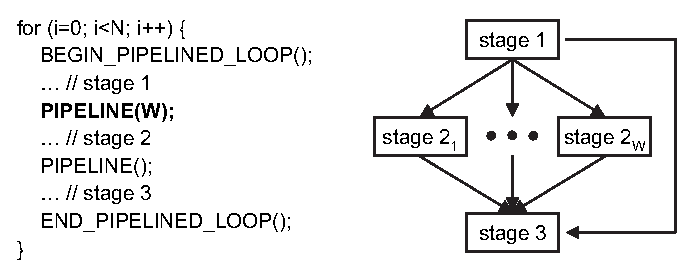
\psfig{file=profiling/data-parallelism.eps,width=3.5in}
\vspace{-6pt}
\caption[Specifying data parallelism.]{Programmers can specify data
  parallelism by passing an extra argument to the pipeline annotation.
  In this case, the runtime system executes W parallel copies of stage
  2.  \protect\label{fig:data-parallelism}}
\vspace{-6pt}
\end{figure}

Once the programmer is satisfied with the parallelism in the stream
graph, the code can automatically be executed in a pipeline-parallel
fashion using the communication macros emitted by the tool.  In most
cases, the macros communicate items from one partition to another
using the corresponding variable name (and potential offset, in the
case of arrays) from the program.  However, a current limitation is in
the case of dynamically-allocated data, where we have yet to automate
the discovery of variable name given the absolute addresses that are
communicated dynamically.  Thus, if the tool detects any communication
of dynamically-allocated data, it alerts the user and indicates the
line of the program that is performing the communication.  The user
needs to supply a symbolic expression for the name and size of the
allocated region.  Only two of our six benchmarks (MPEG-2 and bzip2)
communicate dynamically-allocated data across partition boundaries.
%Fortunately, in streaming applications, dynamically
%allocated data is rarely communicated across partitions, and when it
%is, the shape of the data is relatively simple (e.g., a video frame
%rather than a linked list).  
%
%It is also important to communicate the value of the pointer itself
%between processes, so that each process knows where to receive the
%dynamically allocated data.
%
%Though the frames have a dynamic size, a pointer to the frame is 
% held in a static variable that is easily supplied by the programmer.

\section{Implementation}
\label{sec:parallelization}

\subsection*{Dynamic Analysis Tool}

Our tool is built on top of Valgrind, a robust framework for dynamic
binary instrumentation~\cite{nethercote07valgrind}.  Our analysis
interprets every instruction of the program and (by tracing the line
number in the annotated loop) recognizes which partition it belongs
to.  The analysis maintains a table that indicates, for each memory
location, the identity of the partition (if any) that last wrote to
that location.  On encountering a store instruction, the analysis
records which partition is writing to the location.  Likewise, on
every load instruction, the analysis does a table lookup to determine
the partition that produced the value being consumed by the load.
Every unique producer-consumer relationship is recorded in a list that
is output at the end of the program, along with the stream graph and
communication macros.

There are some interesting consequences of tracking dependence
information in terms of load and store instructions.  In order to
track the flow of data through local variables, we disable register
allocation and other optimizations when preparing the application for
profiling.  However, as we do not model the dataflow through the
registers, the tool is unable to detect cases in which loaded values
are never used (and thus no dependence exists).  This pattern often
occurs for short or unaligned datatypes; even writes to such variables
can involve loads of neighboring bytes, as the entire word is loaded
for modification in the registers.  Our tool filters out such
dependences when they occur in parallel stack frames, i.e., a spurious
dependence between local variables of two neighboring function calls.
Future work could further improve the precision of our reported
dependences by also tracking dependences through registers (in the
style of Redux~\cite{nethercote03redux}).

As the dynamic analysis traces communication in terms of absolute
memory locations, some engineering was required to translate these
addresses to variable names in the generated macros.  (While absolute
addresses could also be used in the macros, they would not be robust
to changes in stack layout or in the face of re-compilation.)  We
accomplish this mapping using a set of gdb scripts\footnote{Our
  scripts rely on having compiled with debug information.}, which
provide the absolute location of every global variable as well as the
relative location of every local variable (we insert a known local
variable and print its location as a reference point).  In generating
the communication code, we express every address as an offset from the
first variable allocated at or below the given location.
%This transformation assumes that the program is memory safe, i.e., it
%does not depend on the relative layout of one variable versus another.
% --> actually some dependence is ok
In the case of dynamically-allocated data, the mapping from memory
location to variable name is not yet automated and requires programmer
assistance (as described in the previous section).

\subsection*{Parallel Runtime System}

The primary challenge in implementing pipeline parallelism is the need
to buffer data between execution stages.  In the sequential version of
the program, a given producer and consumer takes turns in accessing
the shared variables used for communication.  However, in the parallel
version, the producer is writing a given output while the producer is
still reading the previous one.  This demands that the producer and
consumer each have a private copy of the communicated data, so that
they can progress independently on different iterations of the
original loop.  Such a transformation is commonly referred to as
``double-buffering'', though we may wish to buffer more than two
copies to reduce the synchronization between pipeline stages.

There are two broad approaches for establishing a buffer between
pipeline stages: either explicitly modify the code to do the
buffering, or implicitly wrap the existing code in a virtual
environment that performs the buffering automatically.  The first
approach utilizes a shared address space and modifies the code for the
producer or consumer so that they access different locations; values
are copied from one location to the other at synchronization points.
Unfortunately, this approach requires a deep program analysis in order
to infer all of the variables and pointer references that need to be
remapped to shift the produced or consumed data to a new location.
Such an analysis seems largely intractable for a language such as C.

The second approach, and the one that we adopt, avoids the
complexities of modifying the code by simply forking the original
program into multiple processes.  The memory spaces of the processes
are isolated from one another, yet the processes share the exact same
data layout so no pointers or instructions need to be adjusted.  A
standard inter-process communication mechanism (such as pipes) is used
to send and buffer data from one process to another; a producer sends
its latest value for a given location, and the consumer reads that
value into the same location in its private address space.  At the end
of the loop's execution, all of the processes copy their modified data
(as recorded by our tool during the profiling stage) into a single
process that continues after the loop.  Our analysis also verifies
that there is no overlap in the addresses that are sent to a given
pipeline stage; such an overlap would render the program
non-deterministic and would likely lead to incorrect outputs.

\begin{table*}[t]
\begin{center}
{\tenpoint
\begin{tabular}{|l|l|l|l|}
\hline
{\bf Benchmark} & {\bf Description} & {\bf Source} & {\bf Lines of Code} \\ \hline \hline
MPEG-2 & MPEG-2 video decoder & MediaBench~\cite{lee97mediabench} & 10,000 \\ \hline
MP3 & MP3 audio decoder & Fraunhofer IIS~\cite{fraunhofer03mp3} & 5,000 \\ \hline
GMTI  & Ground Moving Target Indicator & MIT Lincoln Laboratory~\cite{reuther03gmti} & 37,000\\ \hline
197.parser & Grammatical parser of English language & SPECINT 2000 & 11,000 \\ \hline
256.bzip2 & bzip2 compression and decompression & SPECINT 2000 & 5,000 \\ \hline
456.hmmer & Calibrating HMMs for biosequence analysis & SPECCPU 2006 & 36,000 \\ \hline
\end{tabular}}
\caption{Benchmark characteristics.\protect\label{tab:prof-benchmarks}}
\end{center}
\end{table*}

% could add:
%  - for "backwards communication" (loop-carried, from later partition to earlier one), 
%    place the receive instruction at the bottom of the partition rather than the top

\section{Case Studies}
\label{sec:results}

To evaluate our approach, we applied our tool and methodology to six
realistic programs.  Three of these are traditional stream programs
(MPEG-2 decoding, MP3 decoding, GMTI radar processing) while three are
SPEC benchmarks (parser, bzip2, hmmer) that also exhibit regular flows
of data.  As illustrated in Table~\ref{tab:prof-benchmarks}, the size of
these benchmarks ranges from 5 KLOC to 37 KLOC.  Each program
processes a conceptually-unbounded stream of input data; our technique
adds pipeline parallelism to the toplevel loop of each application,
which is responsible for 100\% of the steady-state runtime.  (For
bzip2, there are two toplevel loops, one for compression and one for
decompression.)

In the rest of this section, we first describe our experience in
parallelizing the benchmarks before presenting performance results.

\subsection*{Parallelization Experience}

During the parallelization process, the programmer relied heavily on
the stream graphs extracted by our tool.  The final graphs for each
benchmark appear in Figures~\ref{fig:mpeg2-mp3-graphs}
and~\ref{fig:spec-graphs}.  In the graphs, node labels are gleaned
from function names and comments in the code, rather than from any
domain-specific knowledge of the algorithm.  Nodes are also annotated
with the amount of work they perform, while edges are labeled with the
number of bytes communicated per steady-state iteration.  Nodes that
were data-parallelized are annotated with their multiplicity; for
example, the Dequantize stage in MP3
(Figure~\ref{fig:mpeg2-mp3-graphs}b) is replicated twice.

As described in Section~\ref{sec:workflow}, our tool relies on some
programmer assistance to parallelize the code.  The manual steps
required for each benchmark are summarized in
Figure~\ref{fig:program-changes} and detailed in the following
sections.
% summarize comments about print statements here?

%% \begin{figure}[t]
%% \centering
%% \mbox{\hspace{0pt}}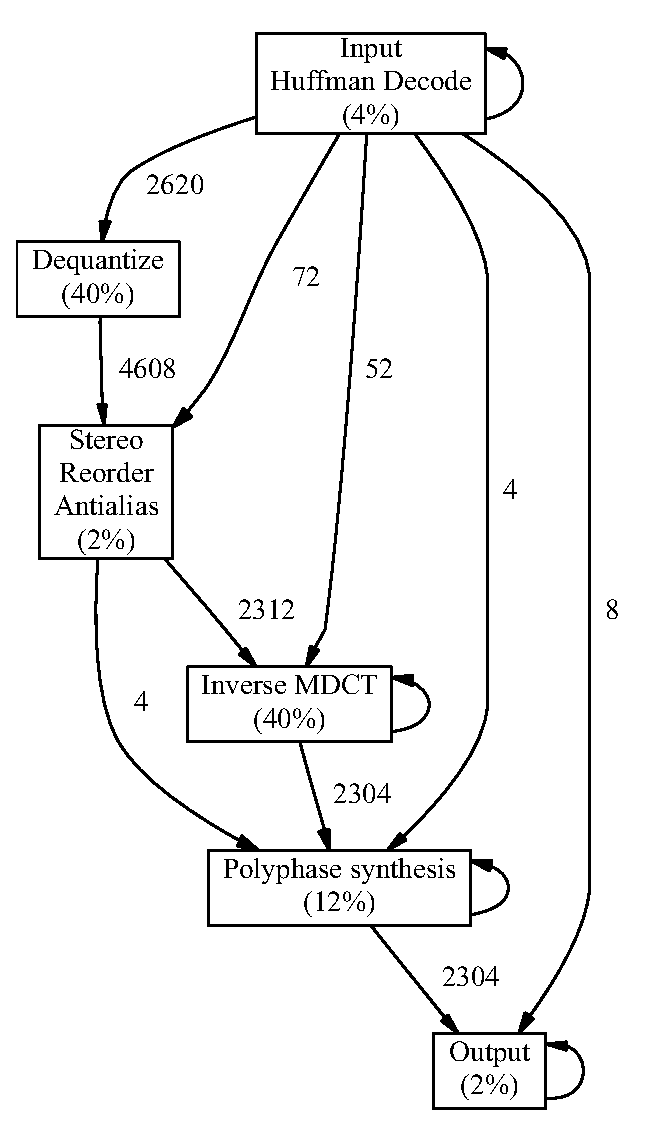
\psfig{file=profiling/mp3-orig.eps,width=1.93in}
%% \caption{Extracted stream graph for MP3 decoder.\protect\label{fig:mp3-graph}}
%% \end{figure}

%% The extracted graph is very similar to a block diagram for GMTI
%% (Figure~\ref{fig:gmti-graph}b) that is provided in the high-level
%% specification for the algorithm~\cite{reuther03gmti}.  By
%% automatically extracting an accurate high-level diagram of the
%% communication pattern, our analysis aids new programmers in
%% understanding and parallelizing the application.

%% \begin{figure}[t]
%% \vspace{-12pt}
%% \centering
%% % 454 pix wide
%% % seem to need the hspace command just to get it to center correctly
%% \hspace{0in}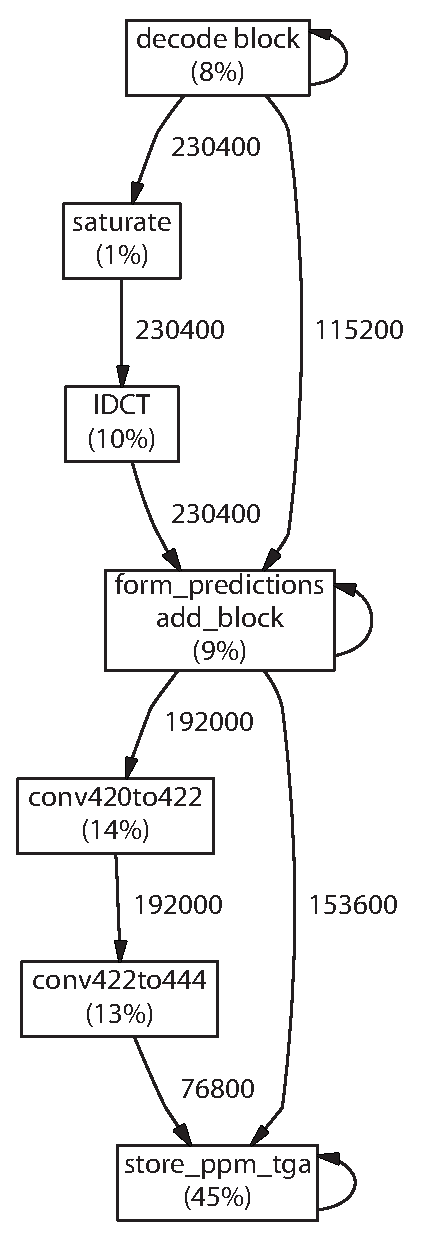
\psfig{file=profiling/mpeg2-opt.eps,width=1.52in}
%% \caption{Extracted stream graph for MPEG-2 decoder.  Nodes are
%%   numbered by their order of appearance in the sequential version of
%%   the code, and also labeled with the percentage of the program's
%%   work that they perform.  Edges are labeled with the number of bytes
%%   transferred per steady state
%%   iteration.\protect\label{fig:mpeg2-graph}}
%% \vspace{-12pt}
%% \end{figure}

\paragraph*{MPEG-2 Decoding} To obtain the stream graph for MPEG-2
(Figure~\ref{fig:mpeg2-mp3-graphs}a), the programmer iteratively
refined the program with the help of the dynamic analysis tool.
Because the desired partition boundaries fell in distinct functions,
those functions were inlined into the main loop.  Early return
statements in these functions led to unstructured control flow after
inlining; the programmer converted the control flow to if/else blocks
as required by our analysis.  The tool exposed an unintended data
dependence that was inhibiting parallelism: a global variable
(progressive\_frame) was being re-used as a temporary variable in one
module.  The programmer introduced a unique temporary variable for
this module, thereby restoring the parallelism.  In addition, the
updates to some counters in the main loop were reordered so as to
place them in the same pipeline stage that the counters were utilized.
%Finally, the programmer turned off an optional tracing flag to reduce
%the verbosity of print statements.  (Removed this because if it's
%optional, then that's just the version of the benchmark we used.)

\begin{figure}[t]
\centering
\vspace{-6pt}
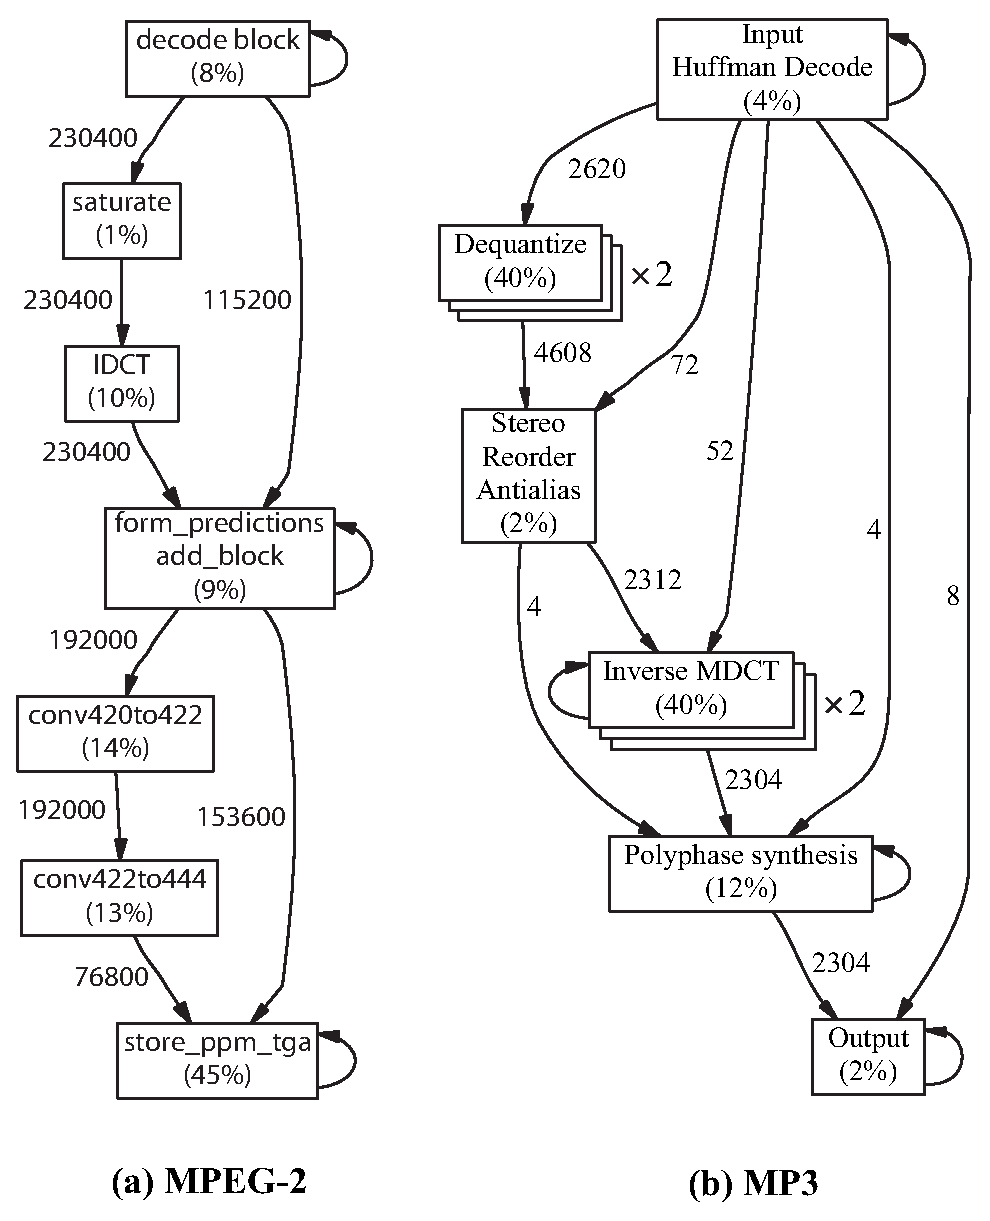
\psfig{file=profiling/mpeg2-mp3-graph.eps,width=3.5in}
\caption{Extracted stream graphs for MPEG-2 and MP3 decoding.\protect\label{fig:mpeg2-mp3-graphs}}
\vspace{-10pt}
\end{figure}

\begin{figure*}[t]
\centering
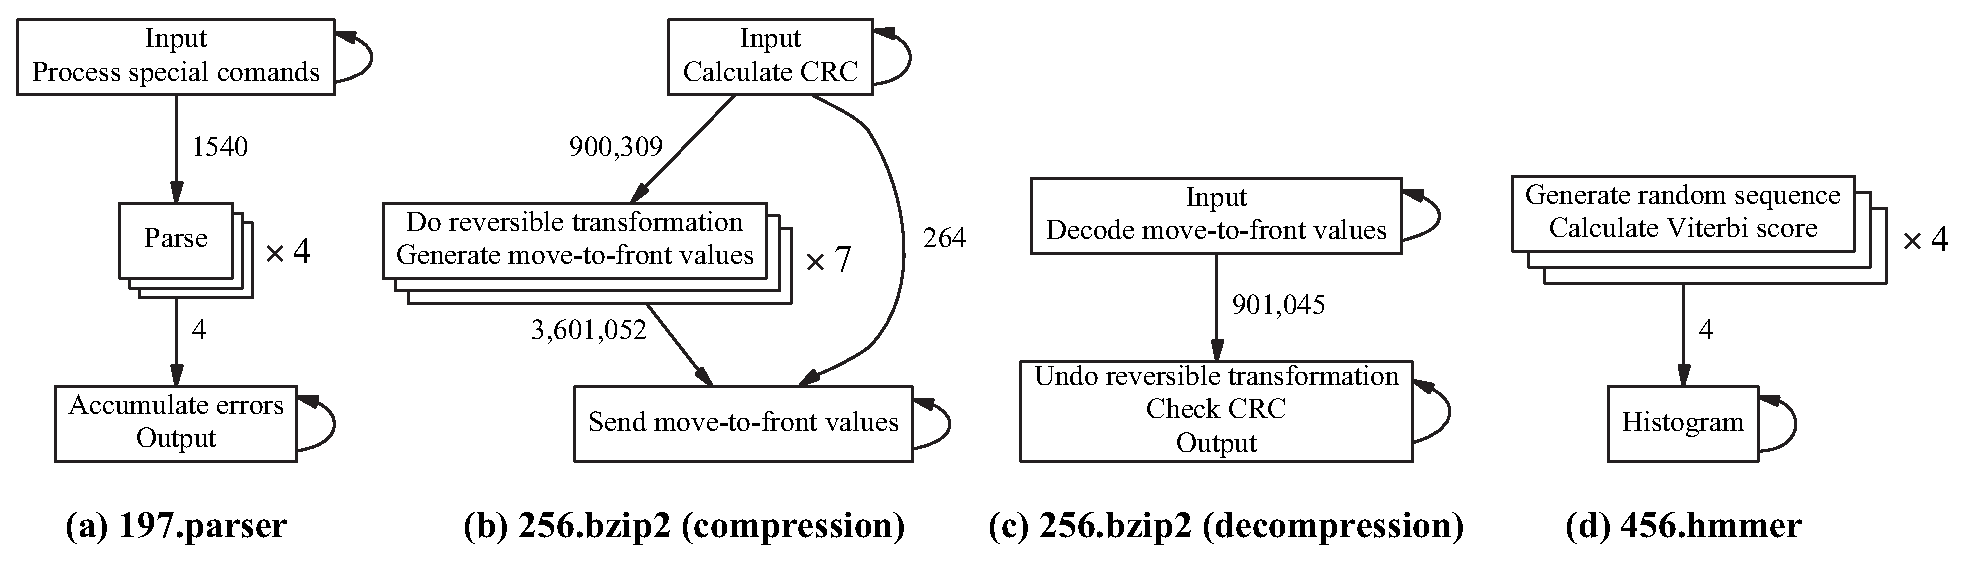
\psfig{file=profiling/spec-graphs.eps,width=\textwidth}
\caption[Extracted stream graphs for parser, bzip2, and
  hmmer.]{Extracted stream graphs for parser, bzip2 (compression and
  decompression) and hmmer.  \protect\label{fig:spec-graphs}}
\end{figure*}

In generating the parallel version, our tool required two
interventions from the programmer.  First, as the pipeline boundaries
spanned multiple loop nests, the communication code (auto-generated
for a single loop nest) was patched to ensure that matching send and
receive instructions executed the same number of times.  Second, as
described in Section~\ref{sec:workflow}, the programmer supplied the
name and size of dynamically-allocated variables (in this case, frame
buffers) that were sent between partitions.

\paragraph*{MP3 Decoding} The extracted stream graph for MP3 decoding
appears in Figure~\ref{fig:mpeg2-mp3-graphs}b.  In the process of
placing the pipeline boundaries, the programmer inlined functions,
unrolled two loops, and distributed a loop.  Four
dynamically-allocated arrays (of fixed size) were changed to use
static allocation, so that our tool could manage the communication
automatically.  As profiling indicated that the dequantization and
inverse MDCT stages were consuming most of the runtime, they were each
data-parallelized two ways.

In analyzing the parallelism of MP3, the programmer made three
deductions.  First, the initial iteration of the loop was found to
exhibit many excess dependences due to one-time initialization of
coefficient arrays; thus, the profiling and parallelization was
postponed to the second iteration.  Second, though the tool reports a
carried dependence in the inverse MDCT stage, the programmer found
that this dependence is on an outer loop and that it is safe to
data-parallelize the stage on an inner loop.  Finally, the programmer
judged the execution to be insensitive to the ordering of diagnostic
print statements, allowing the dependences between statements to be
ignored for the sake of parallelization.  (With some additional
effort, the original ordering of print statements can always be
preserved by extracting the print function into its own pipeline
stage.)

As in the case of MPEG-2, the programmer also patched the generated
communication code to handle nested loops.

\paragraph*{GMTI Radar Processing} The Ground Moving Target Indicator (GMTI)
is a radar processing application that extracts targets from raw radar
data~\cite{reuther03gmti}.  The stream graph extracted by our tool
(Figure~\ref{fig:gmti-graph-tool}) is very similar to the one that
appears in the GMTI specification (Figure~\ref{fig:gmti-graph-spec}).

%It performs adaptive,
%computationally-intensive filtering to minimize the impact of ground
%clutter and interference patterns.  
In analyzing GMTI, the programmer made minor changes to the original
application.  The programmer inlined two functions, removed the
application's self-timers, and scaled down an FFT window from 4096 to
512 during the profiling phase (the resulting communication code was
patched to transfer all 4096 elements during parallel execution).  

As print statements were judged to be independent of ordering, the
tool was instructed to ignore the corresponding dependences.
Dependences between calls to memory allocation functions (malloc/free)
were also disregarded so as to allow pipeline stages to manage their
local memories in parallel.  The programmer verified that regions
allocated within a stage remained private to that stage, thus ensuring
that the parallelism introduced could not cause any memory hazards.

Our tool reported an address trace that was gradually increasing over
time; closer inspection revealed that an array was being read in a
sparse pattern that was gradually encompassing the entire data space.
The programmer directed the tool to patch the parallel version so that
the entire array was communicated at once.

\begin{figure*}[t]
\hspace{-0.25in}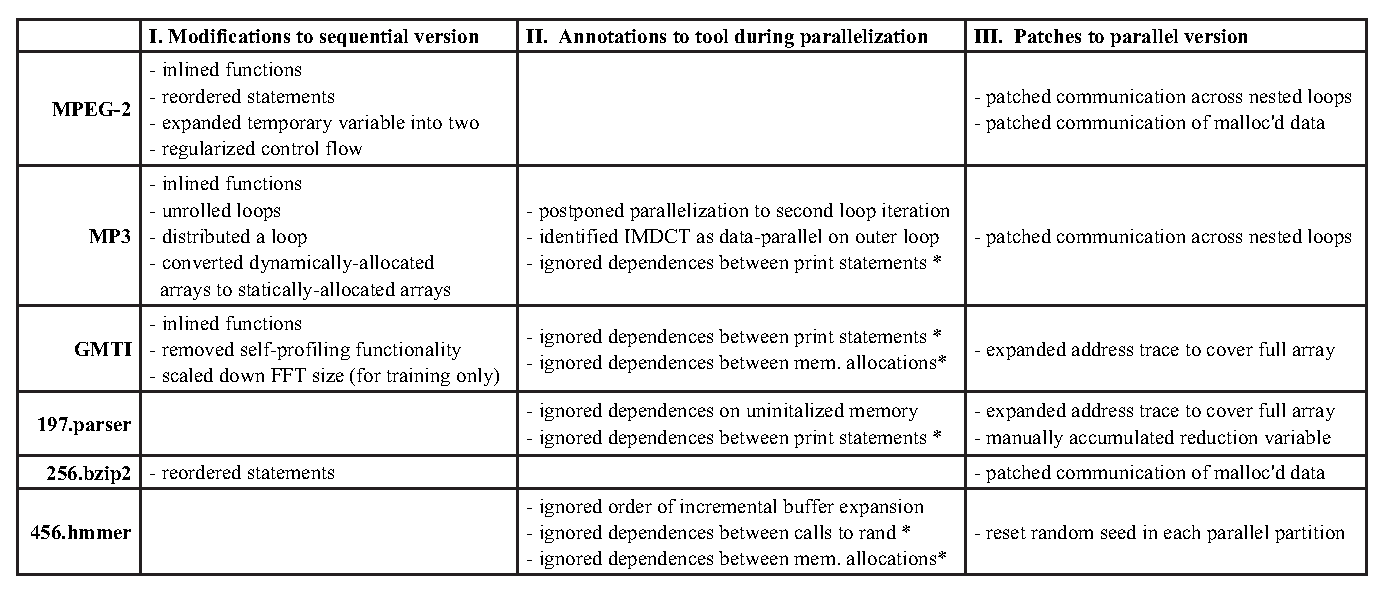
\psfig{file=profiling/program-changes.eps,width=7in}
\caption[Steps taken by programmer to assist with
  parallelization.]{Steps taken by the programmer to assist in
  parallelizing each benchmark.  Assistance may be needed to expose
  parallelism in the original code, to verify parallelism using the
  tool, or to handle special cases in the parallelized code.  Steps
  annotated with an asterisk (*) may change the observable behavior of
  the program\protect\footnotemark[1].
  \protect\label{fig:program-changes}}
\end{figure*}

%% \begin{figure}[t]
%% \centering
%% % seem to need the hspace command just to get it to center correctly
%% \hspace{0in}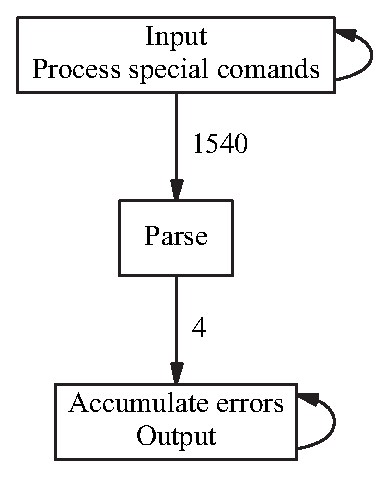
\psfig{file=profiling/parser-orig.eps,width=1.40in}
%% \caption{Original stream graph for 197.parser.  Edges are labeled with
%%   the number of bytes transferred per steady state iteration.  In the
%%   optimized graph (not shown), the Parse stage is duplicated four
%%   times.\protect\label{fig:parser-graph}}
%% \end{figure}

\paragraph*{Parser} The stream graph for 197.parser appears in
Figure~\ref{fig:spec-graphs}a.  Each steady-state iteration of the
graph parses a single sentence; the benchmark runs in batch mode,
repeatedly parsing all of the sentences in a file.  As indicated in
the graph, the cyclic dependences in the benchmark are limited to the
input stage (which performs file reading and adjusts the configuration
of the parser) and the output stage (which accumulates an error
count).  The parsing stage itself (which represents most of the
computation) retains no mutable state from one sentence to the next,
and can thus be replicated to operate on many sentences in parallel.
In our optimized version, the parsing stage is replicated four times.

During the iterative parallelization process, the programmer made
three adjustments to the program.  Our tool reported a number of
loop-carried dependences due to the program's implicit use of
uninitialized memory locations; the program allocates space for a
struct and later copies the struct (by value) before all of the
elements have been initialized.  This causes our tool to report a
dependence on the previous write to the uninitialized locations, even
though such writes were modifying a different data structure that has
since been de-allocated.  The programmer eliminated these dependence
reports by initializing all elements to a dummy value at the time of
allocation.

The programmer also made two adjustments to the communication trace
emitted by our tool.  One block of addresses was expanding gradually
over the first few iterations of the program.  Closer inspection
revealed that that sentences of increasing length were being passed
between partitions.  The programmer patched the trace to always
communicate the complete sentence buffer.
% (1500 characters)
Also, the programmer observed that in the case of errors, the parser's
error count needs to be communicated to the output stage and
accumulated there.  As none of our training or testing samples
elicited errors, our trace did not detect this dependence.

Our data-parallel version of the program may reorder the program's
print statements.  If desired, the print statements can be serialized
by moving them to the output stage.

%% \begin{figure}[t]
%% \centering
%% % seem to need the hspace command just to get it to center correctly
%% \hspace{0in}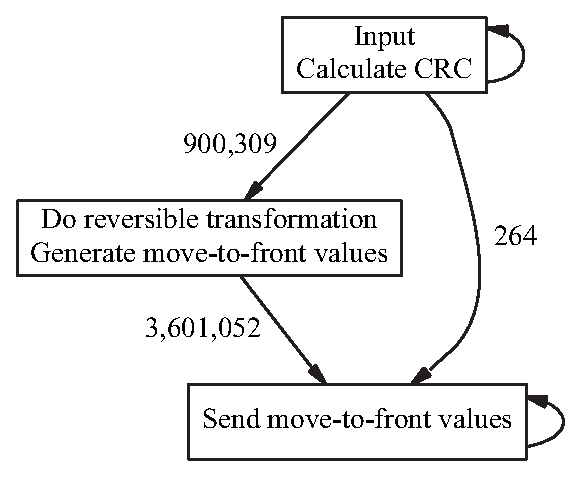
\psfig{file=profiling/bzip2-compress-orig.eps,width=2.15in}
%% \\{\bf (a) bzip2 compression}
%% \\ ~ \\ ~ \\
%% \hspace{0in}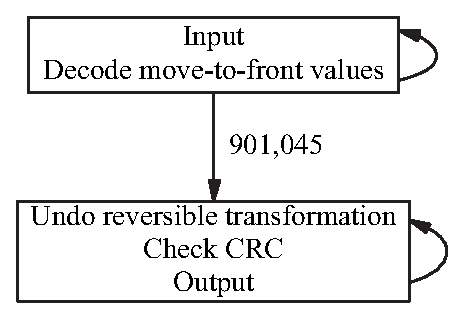
\psfig{file=profiling/bzip2-uncompress-orig.eps,width=1.69in}
%% \\{\bf (b) bzip2 decompression~~~}
%% \\ ~ 
%% \caption{Original stream graphs for 256.bzip2.  Edges are labeled with
%%   the number of bytes transferred per steady state iteration (at
%%   compression level 9).  In the optimized graph (not shown), the
%%   middle stage of the compression step (a) is duplicated seven
%%   times.\protect\label{fig:bzip2-graph}}
%% \vspace{-10pt}
%% \end{figure}

\paragraph*{Bzip2} The stream graphs for 256.bzip2 appear in
Figures~\ref{fig:spec-graphs}b and~\ref{fig:spec-graphs}c.  The
benchmark includes both a compression and decompression stage, which
were parallelized separately.

\footnotetext[1]{Reordering calls to malloc (or reordering calls to
  free) will only change the program's behavior if one of the calls
  fails.}

Because bzip2 compresses blocks of fixed size, the main compression
routine is completely data-parallel.  The only cyclic dependences in
the compressor are at the input stage (file reading, CRC calculation)
and output stage (file writing).  The programmer replicated the
compression stage seven ways to match the four-core machine; this
allows three cores to handle two compression stages each, while one
core handles a single compression stage as well as the input and
output stages.  The decompression step lacks data-parallelism because
the boundaries of the compressed blocks are unknown; however, it can
be split into a pipeline of two stages.

In parallelizing bzip2, the programmer reordered some statements to
improve the pipeline partitioning (the call to {\tt generateMTFValues}
moved from the output stage to the compute stage).  The programmer
also supplied the name and size of two dynamically-allocated arrays.

%This transfer represents a very coarse-grained communication: at
%compression level 9, the compression stage inputs and outputs a total
%of 4.5 MB of data per iteration.  Nonetheless, the compression stage
%exhibits a speedup of 3.07x; there is a 1.78x speedup for the
%decompression stage, and a 2.66x speedup for both stages combined.

%% \begin{figure}[t]
%% \centering
%% % seem to need the hspace command just to get it to center correctly
%% \hspace{0in}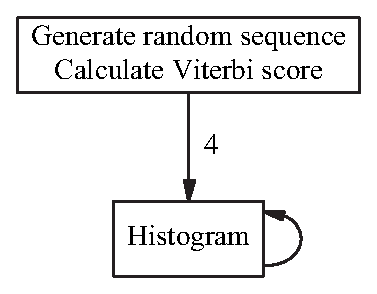
\psfig{file=profiling/hmmer-orig.eps,width=1.35in}
%% \caption{Original stream graph for 456.hmmer.  Edges are labeled with
%%   the number of bytes transferred per steady state iteration.  In the
%%   optimized graph (not shown), the top stage is duplicated four
%%   times.\protect\label{fig:hmmer-graph}}
%% \vspace{-10pt}
%% \end{figure}

\paragraph*{Hmmer} In 456.hmmer, a Hidden Markov Model is loaded at
initialization time, and then a series of random sequences are used to
calibrate the model.  Figure~\ref{fig:spec-graphs}d shows the
extracted stream graph for this benchmark.  The calibration is
completely data-parallel except for a histogram at the end of the
loop, which must be handled with pipeline parallelism.  In our
experiments, the programmer replicated the data-parallel stage four
ways to utilize the four-core machine.

Our tool reports three parallelism-limiting dependences for hmmer.
The first is due to random number generation: each iteration generates
a new random sample and modifies the random seed.  The programmer
chose to ignore this dependence, causing the output of our parallel
version to differ from the original version by 0.01\%.  Also, the
programmer made an important patch to the parallel code: after forking
from the original process, each parallel partition needs to set its
random seed to a different value.  Otherwise each partition would
follow an identical sequence of random values, and the parallel
program would sample only a fraction of the input space as the
original program.

The second problematic dependence is due to an incremental resizing of
an array to fit the length of the input sequence.  Since each parallel
partition can expand its own private array, this dependence is safely
ignored.  Finally, as in the case of GMTI, dependences between memory
allocation functions were relaxed for the sake of the parallelization.

\subsection*{Performance Results}
\label{sec:performance}

Following parallelization with our tool, all of the benchmarks obtain
the correct results on their training and testing sets.  For MPEG-2
and MP3, we train using five iterations of input files 1 and 10,
respectively (see Section~\ref{sec:stability}).  For GMTI, we only
have access to a single input trace, so we use five iterations for
training and the rest (300 iterations) for testing.  For the SPEC
benchmarks, we train on five iterations of the provided training set
and test on the provided testing set.

Our evaluation platform contains two AMD Opteron 270 dual-core
processors (for a total of 4 cores) with 1 MB L2 cache per processor
and 8 GB of RAM.  We measure the speedup of the parallel version,
which uses up to 4 cores, versus the original sequential version,
which uses 1 core.  We generate one process per stage of the stream
graph, and rely on the operating system to distribute the processes
across cores (we do not provide an explicit mapping from threads to
cores).  All speedups reflect total (wall clock) execution time.

Our performance results appear in Table~\ref{tab:results}.  Speedups
range from 2.03x (MPEG-2) to 3.89x (hmmer), with a geometric mean of
{\meanspeedup}.  While these results are good, there is some room for
improvement.  Some benchmarks (MPEG-2, decompression stage of bzip2)
suffer from load imbalance that is difficult to amend without
rewriting parts of the program.  The imperfect speedups in other
benchmarks may reflect synchronization overheads between threads, as
the operating system would need to interleave executions in a specific
ratio to avoid excessive blocking in any one process.  The volume of
communication does not appear to be a significant bottleneck; for
example, duplicating all communication instructions in MP3 results in
only a 1.07x slowdown.  Ongoing work will focus on improving the
runtime scheduling of the processes, as well as exploring other
inter-process communication mechanisms (e.g., using shared memory).

\begin{table}[t]
\begin{center}
{\tenpoint
\begin{tabular}{|l|c|c|c|}
\hline
{\bf Benchmark} & {\bf ~Pipeline Depths} & {\bf Data-Parallel Widths} & {\bf Speedup} \\ \hline \hline
GMTI & 9 & --- & 3.03x \\ \hline
MPEG-2 & 7 & --- & 2.03x \\ \hline
MP3 & 6 & 2,2 & 2.48x \\ \hline
197.parser & 3 & 4 & 2.95x \\ \hline
256.bzip2 & 3,2 & 7 & 2.66x \\ \hline
%256.bzip2 & & & 2.66x \vspace{-4pt} \\ 
%\hspace{3pt}{\small compress} & {\small 3} & {\small 7} & \vspace{0pt}{\small 3.07x} \vspace{-4pt} \\ 
%\hspace{3pt}{\small uncompress} & {\small 2} & --- & \vspace{0pt}{\small 1.78x} \vspace{0pt} \\ \hline
456.hmmer & 2 & 4 & 3.89x \\ \hline
{\bf GeoMean} & & & {\bf {\meanspeedup}} \\ \hline 
\end{tabular}}
\caption[Performance results.]{Characteristics of the parallel stream
  graphs and performance results on a 4-core machine.  Data-parallel
  width refers to the number of ways any data-parallel stage was
  replicated.\protect\label{tab:results}}
\end{center}
\vspace{-10pt}
\end{table}

\section{Related Work}

\subsection*{Static Analysis}

The work most closely related to ours is that of Bridges et
al.~\cite{bridges07revisiting}, which was developed concurrently to
our first publication of this research~\cite{thies-micro07}.  They
exploit pipeline parallelism using the techniques of Decoupled
Software Pipelining~\cite{ottoni05decoupled,rangan04array}.  In
addition, they employ thread-level speculation to speculatively
execute multiple loop iterations in parallel.  Both of our systems
require some assistance from the programmer in parallelizing legacy
applications.  Whereas we annotate spurious dependences within our
tool, they annotate the original source code with a new function
modifier (called ``commutative'') to indicate that successive calls to
the function can be freely reordered.  Such source-level annotations
are attractive (e.g., for malloc/free) and could be integrated with
our approach.  However, our transformations rely on a different
property of these functions, as we call them in parallel from isolated
address spaces rather than reordering the calls in a single address
space.

Once parallelism has been exposed, their compiler automatically places
the pipeline boundaries and generates a parallel runtime, whereas we
rely on the programmer to place pipeline boundaries and to provide
some assistance in generating the parallel version (see
Section~\ref{sec:workflow}).  Our approaches arrive at equivalent
decompositions of 197.parser and 256.bzip2.  However, our runtime
systems differ.  Rather than forking multiple processes that
communicate via pipes, they rely on a proposed ``versioned memory''
system~\cite{vachharajani07speculation} that maintains multiple
versions of each memory location.  This allows threads to communicate
via shared memory, with the version history serving as buffers between
threads.  Their evaluation platform also includes a specialized
hardware construct termed the synchronization
array~\cite{rangan04array}.  In comparison, our technique runs on
commodity hardware.

Dai et al. presents an algorithm for automatically partitioning
sequential packet-processing applications for pipeline-parallel
execution on network processors~\cite{dai05packet}.  
%They formulate
%the problem as a network flow optimization, aiming to balance the
%computation while minimizing communication.  
Their static analysis targets fine-grained instruction sequences
%(represented by a control flow graph in SSA form) 
within a single procedure, while our dynamic analysis is
coarse-grained and inter-procedural.  Du et al. describes a system for
pipeline-parallel execution of Java programs~\cite{du03sc}.  The
programmer declares parallel regions, while the compiler automatically
places pipeline boundaries and infers the communicated variables using
an inter-procedural static analysis.  Unlike our system, the compiler
does not check if the declared regions are actually parallel.

\subsection*{Dynamic Analysis}

The dynamic analysis most similar to ours is that of Rul et
al.~\cite{rul06functionlevel}, which also tracks producer/consumer
relationships between functions and uses the information gleaned to
assist the programmer in parallelizing the program.  They use bzip2 as
a case study and report speedups comparable to ours.  
%The most
%significant difference between our work is the method of
%parallelization: we describe a systematic and semi-automatic process,
%while Rul et al. relies on ad-hoc and manual techniques.  
However, it appears that their system requires the programmer to
determine which variables should be communicated between threads
%while our analysis automatically generates a set of macros to perform
%the needed communication.  Also, they 
and to modify the original program to insert new buffers and
coordinate thread synchronization.
%,
%while we utilize pipes between forked processes to provide transparent
%buffering and synchronization.

Karkowski and Corporaal also utilize dynamic information to uncover
precise dependences for parallelization of C
programs~\cite{karkowski97overcoming}.  Their runtime system utilizes
a data-parallel mapping rather than a pipeline-parallel mapping, and
they place less emphasis on the programmer interface and visualization
tools.

%Also, by forking multiple processes, our approach
%isolates threads from each other, allowing them to proceed
%asynchronously without conflicts in internal state; such conflicts
%would need to be resolved by hand using Rul et al.'s approach.

% TRUE BUT TOO LONG:
%
% - Our analysis is slightly more fine grained, as we track
% communication by line number rather than across function.  Finally,
% we evaluate across six case studies, while they consider only bzip2.
%
% - we also target stream programs, while they target C programs ``with
% limited parallelism''

Redux is a tool that traces instruction-level producer/consumer
relationships for program comprehension and
debugging~\cite{nethercote03redux}.
%for program
%comprehension, debugging, and other
%applications~\cite{nethercote03redux}.  
Unlike our tool, Redux tracks dataflow through registers in addition
to memory locations.  (We avoid the need for such tracking by
profiling an unoptimized binary, generated with gcc -O0, that stores
all intermediate values to memory.)  Because it generates a distinct
graph node for every value produced, the authors note that the
visualization becomes unwieldy and does not scale to realistic
programs.  We address this issue by coarsening the program partitions.
%We also apply the analysis to the
%domain of parallelization.

A style of parallelism that is closely related to pipeline parallelism
is DOACROSS parallelism~\cite{cytron86doacross,padua80highspeed}.
Rather than devoting a processor to a single pipeline stage, DOACROSS
parallelism assigns a processor to execute complete loop iterations,
spanning all of the stages.  In order to support dependences between
iterations, communication is inserted at pipeline boundaries to pass
the loop-carried state between processors.  While DOACROSS parallelism
has been exploited dynamically using inspector/executor models (see
Rauchwerger~\cite{rauchwerger98runtime} for a survey), they lack the
generality needed for arbitrary C programs.  The parallelism and
communication patterns inferred by our tool could be used to generate
a DOACROSS-style mapping; such a mapping could offer improved load
balancing, at the possible expense of degrading instruction locality
and adding communication latency to the critical path.

Giacomoni et al. describe a toolchain for pipeline-parallel
programming~\cite{giacomoni07toolchain}, including BDD-based
compression of dependence traces~\cite{price06bdds}.  Such techniques
could extend our stream graph visualization to a much finer
granularity. 
%There are additional dynamic analyses that offer
%visualizations to aid program
%understanding~\cite{balmas05ddgraph,malton05recovery}, though they do
%not focus on extracting streams of data flow.
DDgraph is a dynamic analysis for Lisp that offers a visualization of
call graphs and data dependence graphs for the sake of program
understanding and correctness checking~\cite{balmas05ddgraph}.  It is
implemented as part of a Lisp interpreter and has been applied to an
AI Blocks World program, which exhibits less regular streams of data
than our target applications.  Malton and Pahelvan also use a dynamic
analysis (built on gdb) to identify control flow between ``pivotal
functions'' that are likely to aid in program
understanding~\cite{malton05recovery}.  They do not extract streams of
data flow.

Program slicing is a technique that aims to identify the set of
program statements that may influence a given statement in the
program.  Slicing is a rich research area with many static and dynamic
approaches developed to date; see Tip~\cite{tip95slice} for a review.
The problem that we consider is more coarse-grained than slicing; we
divide the program into partitions and ask which partitions affect a
given partition.  Also, we identify a list of memory locations that
are sufficient to convey all the information needed between
partitions.  Finally, we are interested only in direct dependences
between partitions, rather than the transitive dependences reported by
slicing tools.

%% object oriented:
%% \cite{leinhard06objflow}
%% \cite{mitchel06modeling}
%%
%% REVERSE ENGINEERING
%% \cite{bellay98reverse}
%%  - evaluates four tools for reverse-engineering C programs
%%  - Refine/C, Imagix4D, SNiFF+, Rigi
%%
%% OTHER COMPILERS:
%%  - other work typically finds data or task parallelism, not pipeline parallelism
%%    - icc gives bad results on our benchmarks
%%  - thread-level speculation (e.g. as cited in August's Auto-thread extraction)
%%  - SUIF?
%%
%% CITE LATER:
%%  \cite{rangan06amortizing} \cite{ram07pipelined}
%%
%%  - Baumstark02 - Exposing Data-Lavel Parallelism in Sequential Image Processing Algorithms
%%  - Baumstark03 - Extracting an Explicitly Data-Parallel Representation of Image-Processing Programs
%%  - Baumstark05 - Retargeting Sequential Image-Processing Programs for Data Parallel Execution
%%  - Chow04 - Understanding Data Lifetime via Whole System Simulation
%%
%%  INFORMATION FLOW - whole directory
%%
%% DON'T CITE:
%% \cite{choi91flowback}

\section{Future Work}

There are rich opportunities for future work in enhancing the
soundness and automation of our tool.  If the runtime system
encounters code that was not visited during training, it could execute
the corresponding loop iteration in a sequential manner (such a policy
would have fixed the only unsoundness we observed).  A static analysis
could also lessen the programmer's involvement, e.g., by automatically
handling nested loops or automatically placing the pipeline
partitions.  Many of the optimizations implemented in StreamIt could
be targeted to the extracted stream graphs, as they follow the
synchronous dataflow model.  It could also be interesting to develop
systematic testing techniques to exhibit control flow paths that were
not covered during training.

More broadly, the observations in Section~\ref{sec:results} suggest
that many of the memory dependences that constrain automatic
parallelizers can be safely ignored without affecting the ultimate
program outcome.  It would be interesting to build a testing tool that
explores this opportunity more deeply, perhaps by systematically
violating each individual memory dependence in the program and
reporting those that do not affect the program outcome.  While such an
analysis would be very slow if only one dependence is broken per run,
perhaps an optimized version can be built by speculatively ``pooling''
many tests into a single run, or by detecting that an intermediate
program state is correct without finishing the complete execution.
Testing tools could also be useful for inferring likely high-level
properties, such as commutativity between methods in a library.  This
would save the user the trouble of indicating the potential for such
reordering to our tool.

\section{Chapter Summary}
\label{sec:conclusions}

This work represents one of the first systematic techniques to extract
a coarse-grained streaming representation from C programs.  Rather
than extracting streams from small instruction sequences or inner
loops, we extract pipeline stages from the outermost toplevel loop of
a streaming application, which encapsulates 100\% of the steady-state
runtime.  Our approach is applicable both to legacy codes, in which
the user has little or no knowledge about the structure of the
program, as well as new applications, in which programmers can utilize
our annotations to easily express the desired pipelining.

The key observation underlying our technique is that for the domain of
streaming applications, the steady-state communication pattern is
regular and stable, even if the program is written in a language such
as C that resists static analysis.  To exploit this pattern, we employ
a dynamic analysis to trace the memory locations communicated between
program partitions at runtime.  Partition boundaries are defined by
the programmer using a simple set of annotations; the partitions can
be iteratively refined to improve the parallelism and load balance.
Our tool uses the communication trace to construct a stream graph for
the application as well as a detailed list of producer-consumer
instruction pairs, both of which aid program understanding and help to
track down any problematic dependences.

Our dynamic analysis tool also outputs a set of macros to
automatically parallelize the program and communicate the needed data
between partitions.  While this transformation is unsound, it is
deterministic and suitable to rigorous testing.  Applying the
transformation to six realistic case studies, the parallel programs
produced the correct output and offered a mean speedup of
{\meanspeedup} on a 4-core machine.
%In addition, the transformation
%proved to be safe for a number of inputs unrelated to our training
%runs; we successfully decoded the top videos from YouTube and the top
%audio tracks from MP3.com.
By leveraging a pragmatic combination of programmer annotations,
dynamic analysis, visualization tools, and parallelization macros, our
approach immediately eases the burden of migrating C applications to a
streaming representation that is suitable for multicore execution.


\section{Conclusions and Future Work}
\label{sec:conclusion}

This paper makes two contributions.  First, it introduces teleport
messaging: a powerful language construct enabling precise message
delivery between nodes of a distributed stream program.  In comparison
with other methods to implement messaging functionality in a
Synchronous Dataflow (SDF) model, teleport messaging is arguably more
readable, more robust, and easier to maintain.  In addition, our
implementation of teleport messaging in the StreamIt compiler resulted
in a 49\% performance improvement for a frequency hopping radio
running on a cluster of workstations.  Like several declarative
language constructs, teleport messaging improves performance by
exposing the true dependences to the compiler and allowing it to
optimize the communication.

%% We outlined several possible applications of $\sdep$, including
%% latency constraints, debugging, speculation, and program analysis, and
%% we look forward to pursuing these directions in the future.

Second, this paper formulates $\sdep$, a natural and useful dependence
representation for the streaming domain.  While this paper applies
$\sdep$ to a new language construct, we envision other applications as
well.  For example, $\sdep$ could be used in a debugger to identify
which iterations of an upstream actor are affecting a given iteration
of a downstream actor.  In a software-based speculation
system~\cite{frank-thesis}, $\sdep$ could be applied to trace the
effects of a failed prediction and to roll back the appropriate actor
executions.  $\sdep$ also offers a new method for measuring latency in
a stream graph.  Similar to representations such as dependence
levels~~\cite{AK82}, direction vectors~\cite{wolfe82}, and dependence
polyhedra~\cite{Irig88} for scientific programs, $\sdep$ provides
dependence information that could be used to test or verify program
transformations.

There are some limitations in the current study that are fertile
grounds for future research.  First, our formulation of $\sdep$
requires a directed path in the stream graph (aligned with the
direction of data flow) between the actors in question.  We are
generalizing $\sdep$ to actors that run in parallel by leveraging
their data dependences with common predecessors (upstream) or
successors (downstream).  Second, as detailed in
Section~\ref{sec:constraints}, we do not solve the general scheduling
problem that incorporates overlapping constraints from teleport
messaging; even determining whether or not a set of constraints is
feasible (especially during the initialization
schedule~\cite{karczma-thesis}) seems to be an interesting question.
Third, in the current model only actors can send and receive messages.
We are extending this into a hierarchical model where stream
containers (such as pipelines) can also receive events and dispatch
them precisely to other streams.  Finally, our approach relies on the
static communication rates present in SDF.  It would be interesting to
consider teleport messaging in a more dynamic context; for example,
downstream non-negative latency messages could be immediately
supported by embedding messages in data items, while other messages
might require speculative delivery or modified timing contracts.

Our work can be viewed as the integration of dynamic behavior into a
static dataflow language.  Our insight is that there is a class of
control messages that only adjust a parameter in the target actor;
they do not otherwise affect the input or output channels upon
delivery.  This model enables a hybrid scheduling scheme in which the
steady-state dataflow is exactly orchestrated at compile time, but
there are windows in which a message could adjust an internal field of
an actor between its execution steps.  We consider this to be a
promising avenue for creating a unified development environment that
captures all aspects of stream application development without
sacrificing either performance or programmability.


\clearpage
\addcontentsline{toc}{chapter}{Bibliography}
{\elevenpoint
\bibliography{references}
\bibliographystyle{amsalpha-abbrv}
}

\appendix
% appears on wrong page
%\addcontentsline{toc}{chapter}{Appendices}
\include{example-program} % have to remove this line during diff
\startchapter{Graphs of StreamIt Benchmarks}
\label{chap:stream-graphs}

\vspace{-\baselineskip}
This appendix contains stream graphs for the StreamIt benchmark suite
(detailed in Table~\ref{tab:lang-benchmarks}).  As described in
Table~\ref{tab:lang-benchmarks-params}, many of the graphs are
parameterized, and we often assign small values to the parameters in
order to facilitate visualization and comprehension of the graph.
Graphs with different sizes, shapes, and work distributions can be
obtained by varying the parameters.

The stream graphs reflect the structure of the original input program,
prior to any transformations by the compiler.  In practice, the
compiler canonicalizes each graph by removing redundant
synchronization points, flattening nested pipelines, and collapsing
data-parallel splitjoins.  With the exception of GMTI and
MPEG2~\footnote{The stream graphs for GMTI and MPEG2 are canonicalized
  by the compiler, in order to reduce their size and improve the
  visualization.}, this canonicalization is disabled to illustrate the
programmer's original intent.

In the stream graphs, each filter is annotated with the following
information:
\begin{itemize}

\item The filter name.\vspace{-3pt}

\item The number of items\footnote{Some items may contain multiple
  values.  For example, if a data channel carries items of array type,
  then the graphs illustrate the number of arrays pushed and popped
  per execution.} pushed and popped per execution of the filter.\vspace{-3pt}

\item The estimated work (number of cycles) per execution of the filter.\vspace{-3pt}

\item Peeking filters are annotated with the number of items peeked (but not popped) per execution.\vspace{-3pt}

\item Stateful filters are annotated as such.

\end{itemize}

Filters are also colored to indicate their approximate amount of work
relative to other filters in the same program.  The heaviest and
lightest filters in a program are assigned fixed colors, and
intermediate filters are colored on a linear scale between the two:

\begin{center}
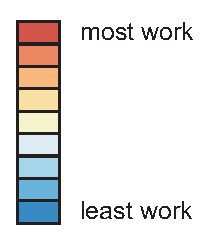
\psfig{file=color-scale.eps, height=1in}
\end{center}

\noindent Work estimates are gathered statically and may differ by 2x 
or more from actual runtime values.  Work estimates are not available
in some programs due to dynamic rates or Java subroutines.  Also, some
individual filters are marked as having ``unknown'' work in cases
where the work estimator is known to perform poorly (while loops,
recursive functions, etc.)

\enlargethispage{0.25\baselineskip}

%%%%%%%%%%%%%%%%%%%%%%%%%%%%%%%%%%%%%%%%%%%%%%%%%%%%%%%%%%%%%%%%%%%%%%%%

% some captions seem to need custom vspace
\newcommand{\tallgraphcustom}[3]{
\clearpage
\begin{figure}[t!]
\vspace{-12pt}
\centering
\psfig{file=apps/#1.eps,height=\textheight}
\vspace{#3}
\caption{Stream graph for #2.\protect\label{fig:#1-graph}}
\vspace{-12pt}
\end{figure}}

% default vspace
\newcommand{\tallgraph}[2]{\tallgraphcustom{#1}{#2}{-12pt}}

\newcommand{\widegraph}[2]{
\clearpage
\begin{figure}[t!]
\vspace{-12pt}
\hspace{-0.025\textwidth}\psfig{file=apps/#1.eps,width=1.05\textwidth}
\vspace{-12pt}
\caption{Stream graph for #2.\protect\label{fig:#1-graph}}
\vspace{-12pt}
\end{figure}}

\newcommand{\smallgraph}[2]{
\clearpage
\begin{figure}[t!]
\vspace{-12pt}
\centering
\psfig{file=apps/#1.eps,scale=0.7}
\vspace{-12pt}
\caption{Stream graph for #2.\protect\label{fig:#1-graph}}
\vspace{-12pt}
\end{figure}}

\tallgraphcustom{3GPP}{3GPP}{-24pt}
\tallgraph{802.11a}{802.11a}
\widegraph{Audiobeam}{Audiobeam}
\widegraph{Autocor}{Autocor}
\smallgraph{BitonicSort-(coarse)}{BitonicSort (coarse)}
\tallgraph{BitonicSort-(fine-iterative)}{BitonicSort (fine, iterative)}
\tallgraph{BitonicSort-(fine-recursive)}{BitonicSort (fine, recursive)}
\tallgraph{BubbleSort}{BubbleSort}
\widegraph{ChannelVocoder}{ChannelVocoder}
\tallgraph{Cholesky}{Cholesky}
\widegraph{ComparisonCounting}{ComparisonCounting}
\tallgraph{CRC}{CRC}
\tallgraph{DCT-(float)}{DCT (float)}
\tallgraph{DCT2D-(NxM-float)}{DCT2D (NxM, float)}
\widegraph{DCT2D-(NxN-int-reference)}{DCT2D (NxN, int, reference)}
\tallgraph{DES}{DES}
\tallgraph{DToA}{DToA}
\tallgraph{FAT}{FAT}
\tallgraph{FFT-(coarse-default)}{FFT (coarse, default)}
\widegraph{FFT-(fine-1)}{FFT (fine 1)}
\widegraph{FFT-(fine-2)}{FFT (fine 2)}
\tallgraph{FFT-(medium)}{FFT (medium)}
\tallgraph{FHR-(feedback-loop)}{FHR (feedback loop)}
\tallgraph{FHR-(teleport-messaging)}{FHR (teleport messaging)}
\widegraph{FMRadio}{FMRadio}
\smallgraph{Fib}{Fib}
\widegraph{FilterBank}{FilterBank}
\tallgraph{GMTI}{GMTI}
\widegraph{GP-particle-system}{GP - particle-system}
\widegraph{GP-phong-shading}{GP - phong-shading}
\widegraph{GP-reference-version}{GP - reference-version}
\widegraph{GP-shadow-volumes}{GP - shadow-volumes}
\widegraph{GSM}{GSM}
\tallgraph{H264-subset}{H264 subset}
\widegraph{HDTV}{HDTV}
\tallgraph{IDCT-(float)}{IDCT (float)}
\tallgraph{IDCT2D-(NxM-float)}{IDCT2D (NxM-float)}
\widegraph{IDCT2D-(NxN-int-reference)}{IDCT2D (NxN, int, reference)}
\smallgraph{IDCT2D-(8x8-int-coarse)}{IDCT2D (8x8, int, coarse)}
\widegraph{IDCT2D-(8x8-int-fine)}{IDCT2D (8x8, int, fine)}
\smallgraph{InsertionSort}{InsertionSort}
\widegraph{JPEG-decoder}{JPEG decoder}
\widegraph{JPEG-transcoder}{JPEG transcoder}
\tallgraph{Lattice}{Lattice}
\widegraph{MP3}{MP3}
\tallgraph{MPD}{MPD}
\tallgraph{MPEG2-decoder}{MPEG2 decoder}
\widegraph{MPEG2-encoder}{MPEG2 encoder}
\widegraph{MatrixMult-(coarse)}{MatrixMult (coarse)}
\widegraph{MatrixMult-(fine)}{MatrixMult (fine)}
\widegraph{MergeSort}{MergeSort}
\widegraph{Mosaic}{Mosaic}
\widegraph{OFDM}{OFDM}
\tallgraph{Oversampler}{Oversampler}
\widegraph{Radar-(coarse)}{Radar (coarse)}
\widegraph{Radar-(fine)}{Radar (fine)}
\tallgraph{RadixSort}{RadixSort}
\smallgraph{RateConvert}{RateConvert}
\smallgraph{Raytracer1}{Raytracer1}
\smallgraph{RayTracer2}{RayTracer2}
\tallgraph{SAR}{SAR}
\tallgraph{SampleTrellis}{SampleTrellis}
\tallgraph{Serpent}{Serpent}
\tallgraph{TDE}{TDE}
\widegraph{TargetDetect}{TargetDetect}
\smallgraph{VectAdd}{VectAdd}
\widegraph{Vocoder}{Vocoder}


\end{document}
